% =====================================================================
%  MCMP113 Introduction to Basic Algorithms and Programming
%  Week 1 Lecture Notes -- Course Introduction, Algorithms, Problem Solving
%  Asst. Prof. Hasan Oguz, PhD -- Istanbul Okan University
%  Compile with XeLaTeX (twice).
%    Student version  : xelatex MCMP113_Week01_Notes.tex
%    Instructor version (with solutions):
%       xelatex -jobname=MCMP113_Week01_Notes_Solutions "\def\withsolutions{1}% =====================================================================
%  MCMP113 Introduction to Basic Algorithms and Programming
%  Week 1 Lecture Notes -- Course Introduction, Algorithms, Problem Solving
%  Asst. Prof. Hasan Oguz, PhD -- Istanbul Okan University
%  Compile with XeLaTeX (twice).
%    Student version  : xelatex MCMP113_Week01_Notes.tex
%    Instructor version (with solutions):
%       xelatex -jobname=MCMP113_Week01_Notes_Solutions "\def\withsolutions{1}% =====================================================================
%  MCMP113 Introduction to Basic Algorithms and Programming
%  Week 1 Lecture Notes -- Course Introduction, Algorithms, Problem Solving
%  Asst. Prof. Hasan Oguz, PhD -- Istanbul Okan University
%  Compile with XeLaTeX (twice).
%    Student version  : xelatex MCMP113_Week01_Notes.tex
%    Instructor version (with solutions):
%       xelatex -jobname=MCMP113_Week01_Notes_Solutions "\def\withsolutions{1}% =====================================================================
%  MCMP113 Introduction to Basic Algorithms and Programming
%  Week 1 Lecture Notes -- Course Introduction, Algorithms, Problem Solving
%  Asst. Prof. Hasan Oguz, PhD -- Istanbul Okan University
%  Compile with XeLaTeX (twice).
%    Student version  : xelatex MCMP113_Week01_Notes.tex
%    Instructor version (with solutions):
%       xelatex -jobname=MCMP113_Week01_Notes_Solutions "\def\withsolutions{1}\input{MCMP113_Week01_Notes.tex}"
% =====================================================================
\documentclass[11pt,a4paper]{article}

% ---------- solutions switch ----------
\newif\ifsolutions
\ifdefined\withsolutions \solutionstrue \else \solutionsfalse \fi

% ---------- fonts ----------
\usepackage{amsmath,amssymb}
\usepackage[sc]{mathpazo}
\usepackage[no-math]{fontspec}
\setmainfont{texgyrepagella}[Extension=.otf,UprightFont=*-regular,BoldFont=*-bold,ItalicFont=*-italic,BoldItalicFont=*-bolditalic]
\setsansfont{texgyreheros}[Extension=.otf,UprightFont=*-regular,BoldFont=*-bold,ItalicFont=*-italic,BoldItalicFont=*-bolditalic]
\IfFontExistsTF{DejaVu Sans Mono}{\setmonofont{DejaVu Sans Mono}[Scale=0.84]}{\setmonofont{lmmono10-regular.otf}}

% ---------- layout ----------
\usepackage[a4paper,margin=2.3cm,headheight=14pt]{geometry}
\usepackage{microtype}
\usepackage{xcolor}
\usepackage{graphicx}
\usepackage{booktabs,tabularx,array,multirow,colortbl}
\usepackage{enumitem}
\usepackage{fancyhdr}
\usepackage{titlesec}
\usepackage[most]{tcolorbox}
\usepackage{listings}
\usepackage{algorithm}
\usepackage[noend]{algpseudocode}
\usepackage{tikz}
\usetikzlibrary{shapes.geometric,shapes.misc,arrows.meta,positioning,calc,fit,decorations.pathreplacing}
\usepackage{hyperref}
\usepackage{needspace}
\renewcommand{\arraystretch}{1.28}
\setlength{\parindent}{0pt}
\setlength{\parskip}{0.55em}

% ---------- colours (same as the slides) ----------
\definecolor{ink}{HTML}{14213D}
\definecolor{amber}{HTML}{FCA311}
\definecolor{amberdk}{HTML}{B7791F}
\definecolor{mist}{HTML}{EEF1F6}
\definecolor{slate}{HTML}{5B6478}
\definecolor{codebg}{HTML}{F4F6FA}
\definecolor{seqc}{HTML}{14213D}
\definecolor{selc}{HTML}{2F6FB3}
\definecolor{repc}{HTML}{2E9E6A}
\definecolor{errc}{HTML}{C8453B}
\hypersetup{colorlinks,linkcolor=ink,urlcolor=selc,citecolor=ink,
  pdftitle={MCMP113 Week 1 Lecture Notes},pdfauthor={Asst. Prof. Hasan Oguz, PhD}}

% ---------- headings ----------
\titleformat{\section}{\sffamily\Large\bfseries\color{ink}}{\color{amber}\texttt{>\_}\hspace{0.4em}\thesection}{0.6em}{}
\titleformat{\subsection}{\sffamily\large\bfseries\color{ink}}{\thesubsection}{0.6em}{}
\titleformat{\subsubsection}{\sffamily\normalsize\bfseries\color{ink}}{}{0em}{}
\titlespacing*{\section}{0pt}{1.6em}{0.6em}
\titlespacing*{\subsection}{0pt}{1.2em}{0.4em}

% ---------- header/footer ----------
\pagestyle{fancy}\fancyhf{}
\fancyhead[L]{\sffamily\small\color{slate}MCMP113 \textperiodcentered{} Introduction to Basic Algorithms and Programming}
\fancyhead[R]{\sffamily\small\color{slate}Week 1\ifsolutions{} \textperiodcentered{} \textcolor{errc}{Instructor edition}\fi}
\fancyfoot[C]{\sffamily\small\color{slate}\thepage}
\renewcommand{\headrulewidth}{0pt}

% ---------- boxes ----------
\newtcolorbox{defbox}[1][]{enhanced,breakable,colback=ink,colframe=ink,coltext=white,
  fonttitle=\sffamily\bfseries,coltitle=amber,title={#1},arc=2mm,boxrule=0pt,left=3mm,right=3mm,top=2mm,bottom=2mm}
\newtcolorbox{notebox}[1][Note]{enhanced,breakable,colback=amber!12,colframe=amber!12,
  fonttitle=\sffamily\bfseries,coltitle=amberdk,title={#1},arc=2mm,boxrule=0pt,left=3mm,right=3mm}
\newtcolorbox{warnbox}[1][Common mistake]{enhanced,breakable,colback=errc!8,colframe=errc!8,
  fonttitle=\sffamily\bfseries,coltitle=errc,title={#1},arc=2mm,boxrule=0pt,left=3mm,right=3mm}
\newtcolorbox{activity}[1][Activity]{enhanced,breakable,colback=mist,colframe=mist,
  fonttitle=\sffamily\bfseries,coltitle=ink,title={#1},arc=2mm,boxrule=0pt,left=3mm,right=3mm}
\newtcolorbox{pseudobox}[1][]{enhanced,colback=codebg,colframe=ink!25,
  fonttitle=\sffamily\small\bfseries,coltitle=ink,colbacktitle=ink!8,title={#1},arc=1.5mm,boxrule=0.4pt,left=2mm,right=2mm,top=1mm,bottom=1mm}
\newtcolorbox{solbox}[1][Solution]{enhanced,breakable,colback=repc!7,colframe=repc!60,
  fonttitle=\sffamily\bfseries,coltitle=white,colbacktitle=repc,title={#1},arc=1.5mm,boxrule=0.5pt}

% ---------- pseudocode conventions ----------
\algrenewcommand\algorithmicif{\textbf{IF}}
\algrenewcommand\algorithmicthen{\textbf{THEN}}
\algrenewcommand\algorithmicelse{\textbf{ELSE}}
\algrenewcommand\algorithmicwhile{\textbf{WHILE}}
\algrenewcommand\algorithmicdo{}
\algrenewcommand\algorithmicfor{\textbf{FOR}}
\algrenewcommand\algorithmicend{\textbf{END}}
\algrenewcommand\algorithmicreturn{\textbf{RETURN}}
\algrenewcommand\alglinenumber[1]{\footnotesize\color{slate}#1}
\newcommand{\READ}{\textbf{READ}\ }
\newcommand{\PRINT}{\textbf{PRINT}\ }
\newcommand{\START}{\State \textbf{START}}
\newcommand{\STOP}{\State \textbf{END}}
\newcommand{\TO}{\ \textbf{TO}\ }
\newcommand{\AND}{\ \textbf{AND}\ }
\newcommand{\OR}{\ \textbf{OR}\ }
\newcommand{\NOT}{\textbf{NOT}\ }
\newcommand{\MOD}{\mathbin{\mathrm{mod}}}
\newcommand{\str}[1]{\texttt{"#1"}}
% explicit END IF / END WHILE / END FOR lines (course convention)
\algdef{SE}[WHILEX]{WhileX}{EndWhileX}[1]{\algorithmicwhile\ #1}{\textbf{END WHILE}}
\algdef{SE}[IFX]{IfX}{EndIfX}[1]{\algorithmicif\ #1\ \algorithmicthen}{\textbf{END IF}}
\algdef{Ce}[ELSEX]{IFX}{ElseX}{EndIfX}{\algorithmicelse}
\algdef{SE}[FORX]{ForX}{EndForX}[1]{\algorithmicfor\ #1}{\textbf{END FOR}}

% ---------- C# listings ----------
\lstdefinelanguage{CSharp14}{language=[Sharp]C,
  morekeywords={var,string,double,int,bool,decimal,if,else,while,for,foreach,return,true,false,using,static,void,new},
  sensitive=true}
\lstset{language=CSharp14,basicstyle=\ttfamily\small,keywordstyle=\color{selc}\bfseries,
  stringstyle=\color{repc!80!black},commentstyle=\color{slate}\itshape,
  backgroundcolor=\color{codebg},frame=single,rulecolor=\color{ink!25},framesep=4pt,xleftmargin=6pt,xrightmargin=6pt,
  numbers=left,numberstyle=\scriptsize\color{slate},numbersep=8pt,showstringspaces=false,
  columns=fullflexible,keepspaces=true,upquote=true,breaklines=true,aboveskip=0.8em,belowskip=0.8em}
\lstdefinestyle{shell}{language={},numbers=none,basicstyle=\ttfamily\small\color{white},backgroundcolor=\color{ink},rulecolor=\color{ink}}

% ---------- misc ----------
\newcommand{\kw}[1]{\textsf{\bfseries #1}}
\newcommand{\term}[1]{\textbf{\color{ink}#1}}
\newcommand{\solution}[1]{\ifsolutions\begin{solbox}#1\end{solbox}\fi}
\newcolumntype{L}{>{\raggedright\arraybackslash}X}
\newcommand{\hdr}[1]{\textcolor{white}{\sffamily\bfseries #1}}
\newcommand{\hrow}{\rowcolor{ink}}
\newcommand{\stars}[1]{\textcolor{amberdk}{\ifcase#1\or$\star$\or$\star\star$\or$\star\star\star$\fi}}

\tikzset{
  fc/.style={draw=ink,line width=0.7pt,align=center,font=\sffamily\small,minimum height=7mm},
  term/.style={fc,rounded rectangle,fill=amber!18,minimum width=20mm},
  io/.style={fc,trapezium,trapezium left angle=72,trapezium right angle=108,trapezium stretches=true,fill=white,minimum width=24mm},
  proc/.style={fc,rectangle,fill=white,minimum width=22mm},
  dec/.style={fc,diamond,aspect=2,fill=selc!10,inner sep=1pt},
  arr/.style={-{Stealth[length=2.2mm]},draw=ink,line width=0.7pt},
}

% =====================================================================
\begin{document}

% ---------------- title block ----------------
\begin{tcolorbox}[enhanced,colback=ink,colframe=ink,arc=3mm,boxrule=0pt,left=6mm,right=6mm,top=5mm,bottom=5mm]
\begin{minipage}[c]{0.74\linewidth}
{\ttfamily\bfseries\color{amber}>\_ MCMP113}\\[2mm]
{\sffamily\bfseries\LARGE\color{white}Introduction to Basic Algorithms\\[1mm] and Programming}\\[3mm]
{\sffamily\large\color{white!80!ink}Week 1 Lecture Notes: Course Introduction,\\ the Concept of an Algorithm, and Problem-Solving Steps}\\[4mm]
{\sffamily\small\color{white}\textbf{Asst.\ Prof.\ Hasan Oğuz, PhD}\\
\color{white!75!ink}Istanbul Okan University \textperiodcentered{} Vocational School \textperiodcentered{} 2026--2027 Fall}
\ifsolutions\\[2mm]{\sffamily\small\bfseries\color{amber}INSTRUCTOR EDITION -- contains solutions}\fi
\end{minipage}\hfill
\begin{minipage}[c]{0.22\linewidth}\centering
\end{minipage}
\end{tcolorbox}

\vspace{2mm}
\begin{notebox}[How to use these notes]
These notes follow the Week~1 slides and add the details that do not fit on a slide: full explanations, every worked example with its trace table, a pseudocode reference card, an English--Turkish glossary and graded exercises. Week~1 is \emph{conceptual}: we do not write C\# yet. Read Sections~\ref{sec:computer}--\ref{sec:problem} before Week~2, then do the exercises in Section~\ref{sec:exercises}.
\end{notebox}

{\small\tableofcontents}

% =====================================================================
\section{About the course}\label{sec:course}

\subsection{Aims and learning outcomes}
MCMP113 teaches you to \emph{think like a programmer}: to turn a problem stated in everyday language into a precise sequence of steps, and then into a working C\# console application. By the end of the semester you should be able to:
\begin{enumerate}[leftmargin=*,itemsep=1pt]
  \item \term{Think algorithmically}: break a real problem into precise, finite, ordered steps.
  \item \term{Draw and read flowcharts}: express an algorithm visually before writing any code.
  \item \term{Write C\# console applications} using variables, operators, decisions and loops correctly.
  \item \term{Work with arrays}: store, search, sort and process collections of data.
  \item \term{Structure programs with functions} that take parameters and return values.
  \item \term{Test and debug}: trace code by hand and locate errors systematically.
\end{enumerate}
Outcomes~1--2 do not depend on any programming language. They are the real skill; C\# is the vehicle we use to practise it.

\subsection{Weekly plan}
\begin{center}\small
\begin{tabularx}{\linewidth}{>{\centering\arraybackslash}p{9mm}L>{\raggedright\arraybackslash}p{38mm}}
\hrow \hdr{Week} & \hdr{Topic} & \hdr{Preparation}\\
\rowcolor{amber!15} 1 & Course introduction \textperiodcentered{} the concept of an algorithm \textperiodcentered{} problem-solving steps & Lecture notes\\
2 & Flowcharts and their symbols \textperiodcentered{} basic flowchart examples & Lecture notes\\
\rowcolor{mist} 3 & Introduction to programming languages \textperiodcentered{} variables \textperiodcentered{} data types \textperiodcentered{} constants & Notes, sample code\\
4 & Arithmetic, logical and relational operators & Notes, sample code\\
\rowcolor{mist} 5 & Decision structures: \texttt{if-else}, \texttt{if-else if}, \texttt{switch-case} & Notes, sample code\\
6 & Loops: the \texttt{for} loop & Notes, sample code\\
\rowcolor{mist} 7 & Loops: \texttt{while} and \texttt{do-while} & Notes, sample code\\
\rowcolor{ink} \textcolor{amber}{\bfseries 8} & \textcolor{white}{\bfseries MIDTERM EXAM} & \textcolor{white}{Review weeks 1--7}\\
9 & One-dimensional arrays: declaration, assignment, element access & Notes, sample code\\
\rowcolor{mist} 10 & Array operations: searching, sorting, finding the maximum/minimum & Notes, sample code\\
11 & Multi-dimensional arrays (matrices) & Notes, sample code\\
\rowcolor{mist} 12 & Functions: definition, calling, parameter passing & Notes, sample code\\
13 & Value-returning and \texttt{void} functions \textperiodcentered{} scope & Notes, sample code\\
\rowcolor{mist} 14 & Basic file operations \textperiodcentered{} semester review & Lecture notes\\
\rowcolor{ink} \textcolor{amber}{\bfseries 15} & \textcolor{white}{\bfseries FINAL EXAM} & \textcolor{white}{Review all topics}\\
\end{tabularx}
\end{center}

\subsection{Assessment and attendance}
\begin{center}
\begin{tabular}{lcc}
\toprule
Component & Week & Weight\\ \midrule
Midterm exam & 8 & $40\%$\\
Final exam & 15 & $60\%$\\ \bottomrule
\end{tabular}
\end{center}
Both exams test \emph{reasoning}: tracing algorithms, drawing flowcharts, and writing short programs by hand. The weekly exercises are not graded, but they are the most direct preparation for the exams. Attendance follows the university regulations.

\subsection{Software (install before Week 3)}
All tools are free and run on Windows, macOS and Linux.
\begin{itemize}[leftmargin=*,itemsep=1pt]
  \item \textbf{.NET 10 SDK} (the current long-term-support release): \url{https://dotnet.microsoft.com/en-us/download/dotnet/10.0}
  \item \textbf{Visual Studio Code}: \url{https://code.visualstudio.com/}
  \item \textbf{C\# Dev Kit} extension for VS Code (search ``C\# Dev Kit'' in the Extensions panel).
\end{itemize}
Check your installation in a terminal (the exact version number may differ):
\begin{lstlisting}[style=shell]
> dotnet --version
10.0.100
> dotnet new console -n Hello
> cd Hello
> dotnet run
Hello, World!
\end{lstlisting}
\begin{notebox}[Why .NET 10 and not .NET 8?]
Support for .NET~8 ends in November 2026, in the middle of our semester; .NET~10 is supported until November 2028. Code written in this course runs on both, but install~10.
\end{notebox}

% =====================================================================
\section{How a computer solves problems}\label{sec:computer}

\subsection{Input -- Process -- Output}
Every program, from a calculator to a video game, follows the same pattern (Figure~\ref{fig:ipo}): data comes \term{in}, the processor \term{processes} it by following instructions, and results go \term{out}.

\begin{figure}[h]\centering
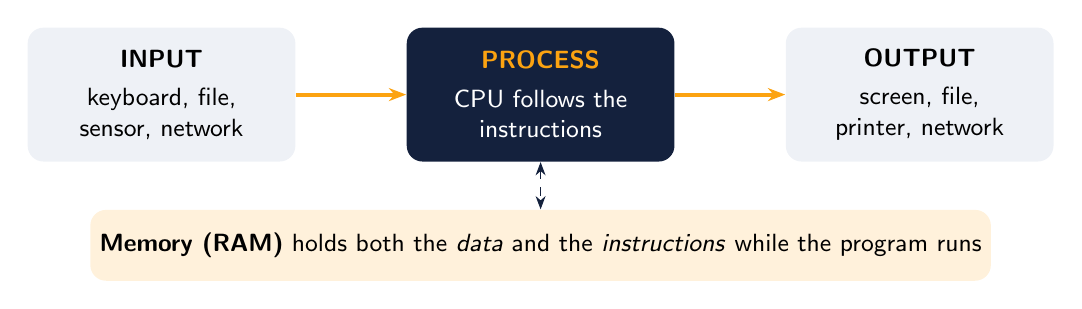
\begin{tikzpicture}[node distance=14mm,
  blk/.style={draw=none,rounded corners=2mm,minimum width=34mm,minimum height=17mm,align=center,font=\sffamily\small}]
\node[blk,fill=mist] (i) {\textbf{INPUT}\\[1mm] keyboard, file,\\ sensor, network};
\node[blk,fill=ink,text=white,right=of i] (p) {\textbf{\color{amber}PROCESS}\\[1mm] CPU follows the\\ instructions};
\node[blk,fill=mist,right=of p] (o) {\textbf{OUTPUT}\\[1mm] screen, file,\\ printer, network};
\draw[arr,draw=amber,line width=1.4pt] (i)--(p); \draw[arr,draw=amber,line width=1.4pt] (p)--(o);
\node[blk,fill=amber!15,below=6mm of p,minimum width=112mm,minimum height=9mm] (m) {\textbf{Memory (RAM)} holds both the \emph{data} and the \emph{instructions} while the program runs};
\draw[<->,>=Stealth,draw=ink,dashed] (p)--(m);
\end{tikzpicture}
\caption{The input--process--output model and the stored-program (von Neumann) idea.}\label{fig:ipo}
\end{figure}

The idea that the program's instructions are stored in the same memory as its data is due to John von Neumann (1945) and is still the architecture of every laptop and phone. RAM is \emph{volatile}: when the power is off it is empty, whereas files on a disk or SSD remain.

\subsection{Fast, but completely literal}
A single modern processor core executes on the order of $10^{9}$ simple instructions per second. Yet every one of those instructions belongs to only four families:
\begin{enumerate}[leftmargin=*,itemsep=1pt]
  \item \textbf{arithmetic} (add, subtract, multiply, divide),
  \item \textbf{comparison and logic} (is $a<b$? AND, OR, NOT),
  \item \textbf{data movement} (copy a value from memory to a register and back),
  \item \textbf{jumps} (continue at another instruction, possibly only if a condition holds).
\end{enumerate}
The computer never guesses what you \emph{meant}. It does exactly what it is told, in exactly the order it is told. Consequently:

\begin{defbox}[Key insight]
The difficult part of programming is not typing code. It is deciding the exact, unambiguous sequence of steps that solves the problem, the \textbf{algorithm}. The programming language only writes those steps in a form the machine can execute.
\end{defbox}

\subsection{From an idea to a running program}
Figure~\ref{fig:pipeline} shows what happens to your work. You write the first two boxes; the tools do the rest when you type \texttt{dotnet run}.

\begin{figure}[h]\centering
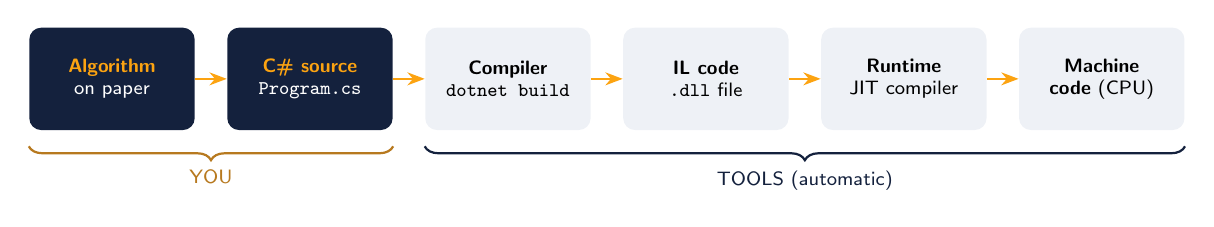
\begin{tikzpicture}[node distance=4mm,
  st/.style={rounded corners=1.5mm,minimum width=21mm,minimum height=13mm,align=center,font=\sffamily\scriptsize}]
\node[st,fill=ink,text=white] (a) {\textbf{\color{amber}Algorithm}\\ on paper};
\node[st,fill=ink,text=white,right=of a] (b) {\textbf{\color{amber}C\# source}\\ \texttt{Program.cs}};
\node[st,fill=mist,right=of b] (c) {\textbf{Compiler}\\ \texttt{dotnet build}};
\node[st,fill=mist,right=of c] (d) {\textbf{IL code}\\ \texttt{.dll} file};
\node[st,fill=mist,right=of d] (e) {\textbf{Runtime}\\ JIT compiler};
\node[st,fill=mist,right=of e] (f) {\textbf{Machine}\\ \textbf{code} (CPU)};
\foreach \x/\y in {a/b,b/c,c/d,d/e,e/f} \draw[arr,draw=amber] (\x)--(\y);
\draw[decorate,decoration={brace,mirror,amplitude=5pt},thick,amberdk] ([yshift=-2mm]a.south west)--([yshift=-2mm]b.south east) node[midway,below=5pt,font=\sffamily\scriptsize,amberdk]{YOU};
\draw[decorate,decoration={brace,mirror,amplitude=5pt},thick,ink] ([yshift=-2mm]c.south west)--([yshift=-2mm]f.south east) node[midway,below=5pt,font=\sffamily\scriptsize,ink]{TOOLS (automatic)};
\end{tikzpicture}
\caption{The C\# tool chain. IL = Intermediate Language; JIT = just-in-time compilation.}\label{fig:pipeline}
\end{figure}

The C\# compiler (called Roslyn) translates source code into \term{Intermediate Language} (IL), stored in a \texttt{.dll} file. When the program starts, the .NET runtime translates the IL into machine code for the actual processor (x64, ARM64, \dots). This is why the same compiled program runs on Windows, Linux and macOS.

\begin{table}[h]\centering\small
\begin{tabularx}{\linewidth}{lp{42mm}L}
\toprule
Level & Example: ``put 5 in a register, add 3'' & Characteristics\\ \midrule
Machine code (x86, hex) & \texttt{B8 05 00 00 00}\newline\texttt{83 C0 03} & The bytes the CPU actually reads. Practically unreadable for humans.\\
Assembly & \texttt{mov eax, 5}\newline\texttt{add eax, 3} & One mnemonic per machine instruction; tied to one processor family.\\
High-level (C\#) & \texttt{int sum = 5 + 3;} & Close to human thinking; portable across systems.\\ \bottomrule
\end{tabularx}
\caption{The same computation at three levels of abstraction.}
\end{table}

\begin{activity}[Think about it]
For each of the following, name the input, the process and the output: a pocket calculator; an ATM withdrawal; a navigation app computing a route; a thermostat.
\end{activity}

% =====================================================================
\section{What is an algorithm?}\label{sec:algorithm}

\subsection{The Exact Instructions Challenge}
In class we watch a short video in which children write instructions for making a sandwich, and their father follows them \emph{literally}: ``put the peanut butter on the bread'' results in the closed jar being placed on the loaf. While watching, note down (i)~which instruction was ambiguous, (ii)~which step was missing, (iii)~which step was in the wrong order, (iv)~whether the ``algorithm'' ever ended, and (v)~how the children fixed it. The father behaves exactly like a processor, and the children's cycle of \emph{write, test, fail, fix} is exactly how programs are developed.

\subsection{Definition}
\begin{defbox}[Definition -- Algorithm]
An \textbf{algorithm} is a \textcolor{amber}{\textbf{finite}} sequence of \textcolor{amber}{\textbf{well-defined}} steps that transforms a given \textcolor{amber}{\textbf{input}} into the desired \textcolor{amber}{\textbf{output}}, and then stops.
\end{defbox}

\paragraph{Where the word comes from.} Muhammad ibn Mūsā al-Khwārizmī (c.\,780--850) worked at the House of Wisdom in Baghdad. His book on calculating with Hindu--Arabic numerals introduced the decimal system to Europe, where his name was Latinised as \emph{Algoritmi}; hence \emph{algorithm}. The title of his other book, \emph{al-Jabr}, gave us the word \emph{algebra}.

\paragraph{Algorithm versus program.} An algorithm is an \emph{idea}, independent of any language; it can be written in words, in pseudocode or as a flowchart. A \term{program} is one \emph{implementation} of that idea in a particular programming language. One algorithm can be implemented in C\#, Python, Java or any other language: the relation is one-to-many. A recipe is an algorithm; the dish cooked in a particular kitchen is a program run.

\subsection{The five properties of an algorithm}
Following D.\,E.~Knuth, a procedure qualifies as an algorithm only if it has all five properties below.

\begin{center}\small
\begin{tabularx}{\linewidth}{>{\bfseries}p{27mm}L>{\leavevmode\itshape\color{errc}}p{47mm}}
\hrow \hdr{Property} & \hdr{Meaning} & \hdr{Violated by \dots}\\
Finiteness & It stops after a finite number of steps. & ``Keep stirring.'' (until when?)\\
\rowcolor{mist} Definiteness & Every step is precise and unambiguous. & ``Add some sugar.'' (how much?)\\
Input & It has zero or more clearly specified inputs. & ``Take the bread.'' (which bread?)\\
\rowcolor{mist} Output & It produces at least one result related to the input. & An empty plate.\\
Effectiveness & Every step is basic enough to be carried out exactly. & ``Make it tasty.''\\
\end{tabularx}
\end{center}

For practical programming we add a sixth requirement: \term{correctness}. The algorithm must produce the right output for \emph{every} valid input, including unusual ones (the \emph{edge cases}).

\subsection{Quiz: algorithm or not?}
Decide for each item whether it is an algorithm. If not, name the property that fails.
\begin{enumerate}[leftmargin=*,itemsep=1pt]
  \item The instructions on a shampoo bottle: ``Lather. Rinse. Repeat.''
  \item The long-division method you learned in primary school.
  \item ``Print the largest prime number.''
  \item A recipe step: ``Add salt to taste.''
  \item Finding a word in a paper dictionary by opening it near the word's first letter and moving forwards or backwards.
  \item ``Choose the best football team in the world.''
\end{enumerate}
\begin{notebox}[Answers]
(1)~No: it never stops (finiteness). (2)~Yes. (3)~No: Euclid proved that there are infinitely many primes, so no largest one exists; the procedure never finishes and produces no output. (4)~No: ``to taste'' is not precise (definiteness). (5)~Yes: the dictionary is finite and alphabetically ordered, so the search always ends. This is the idea behind \emph{binary search} (Week~10). (6)~No: there is no agreed criterion (definiteness, effectiveness).
\end{notebox}

\subsection{An everyday algorithm: brewing Turkish tea}
Compare the vague version ``boil water, add tea, serve'' with the precise version below. The colours mark the three kinds of structure discussed in the next subsection.

\begin{pseudobox}[Algorithm 1 -- Brewing Turkish tea]
\begin{enumerate}[leftmargin=*,itemsep=0pt]
  \item Fill the kettle (bottom pot) with 1\,L of water.
  \item Put 4 teaspoons of black tea into the teapot (top pot).
  \item Place the teapot on the kettle and turn the stove on.
  \item \textcolor{repc}{\textbf{WHILE} the water is not boiling: wait 1 minute.}
  \item Pour boiling water into the teapot until it is $\tfrac34$ full.
  \item Lower the heat and wait 15 minutes.
  \item \textcolor{selc}{\textbf{IF} the guest wants strong tea \textbf{THEN} fill the glass $\tfrac23$ with tea, \textbf{ELSE} fill it $\tfrac13$ with tea.}
  \item Top up the glass with hot water. \textbf{STOP}.
\end{enumerate}
\end{pseudobox}

\subsection{Three structures are enough}
Every algorithm can be built from only three control structures. This is the \term{structured program theorem} of B\"ohm and Jacopini (1966).

\begin{center}\small
\begin{tabularx}{\linewidth}{>{\bfseries}p{24mm}L>{\raggedright\arraybackslash}p{44mm}c}
\hrow \hdr{Structure} & \hdr{Meaning} & \hdr{Pseudocode example} & \hdr{C\# in}\\
\textcolor{seqc}{Sequence} & Steps executed one after another, top to bottom. & \READ $a$, $b$\newline $s\gets a+b$\newline \PRINT $s$ & Weeks 3--4\\
\rowcolor{mist}\textcolor{selc}{Selection} & Choose between paths according to a condition. & \textbf{IF} $age\ge 18$ \textbf{THEN}\newline\hspace*{3mm}\PRINT\str{adult}\newline\textbf{ELSE} \PRINT\str{minor} & Week 5\\
\textcolor{repc}{Repetition} & Repeat a block while a condition holds. & \textbf{WHILE} $i\le 10$\newline\hspace*{3mm}\PRINT $i$;\ $i\gets i+1$ & Weeks 6--7\\
\end{tabularx}
\end{center}
This theorem is why the course is ordered the way it is: after sequence, selection and repetition you have, in principle, everything needed to express any computation.

\subsection{Four ways to write an algorithm}
The same algorithm, ``read a number and print its absolute value'', can be written in four ways:

\begin{center}
\begin{minipage}[t]{0.47\linewidth}
\textbf{(a) Natural language.} \emph{Read the number. If it is negative, remove its minus sign. Show the number.}\\[1mm]
{\small Easy for anyone to read, but often ambiguous.}

\medskip
\textbf{(b) Pseudocode.}\vspace{-2mm}
\begin{pseudobox}
\begin{algorithmic}[1]
\START
\State \READ $x$
\IfX{$x<0$}
  \State $x \gets -x$
\EndIfX
\State \PRINT $x$
\STOP
\end{algorithmic}
\end{pseudobox}
{\small Precise and needs no tools; our main notation on paper.}
\end{minipage}\hfill
\begin{minipage}[t]{0.47\linewidth}
\textbf{(c) Flowchart} (Week~2).\\[1mm]
\centering
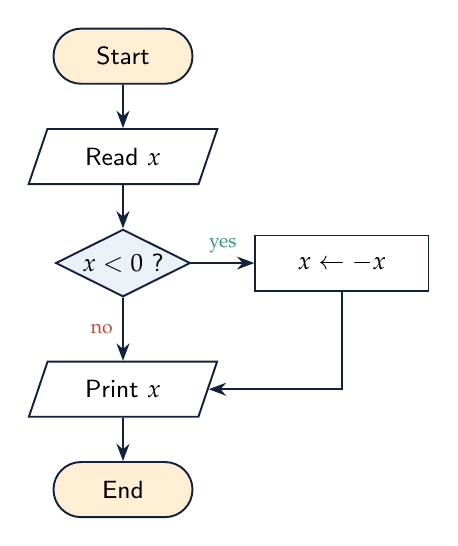
\begin{tikzpicture}[node distance=5.5mm]
\node[term] (s) {Start};
\node[io,below=of s] (r) {Read $x$};
\node[dec,below=of r] (d) {$x<0$ ?};
\node[proc,right=8mm of d] (n) {$x \gets -x$};
\node[io,below=8mm of d] (p) {Print $x$};
\node[term,below=of p] (e) {End};
\draw[arr] (s)--(r); \draw[arr] (r)--(d);
\draw[arr] (d)--node[above,font=\scriptsize,repc]{yes}(n);
\draw[arr] (d)--node[left,font=\scriptsize,errc]{no}(p);
\draw[arr] (n)|-(p);
\draw[arr] (p)--(e);
\end{tikzpicture}
\end{minipage}
\end{center}

\needspace{8\baselineskip}
\textbf{(d) C\# code} (Week~3 onwards). Executable, but with strict syntax:
\begin{lstlisting}
int x = int.Parse(Console.ReadLine());
if (x < 0)
    x = -x;
Console.WriteLine(x);
\end{lstlisting}

\subsection{Pseudocode conventions for MCMP113}\label{sec:conventions}
There is no single standard pseudocode. In this course, in all slides, homework and exams, we use the following conventions.

\begin{center}\small
\begin{tabularx}{\linewidth}{>{\ttfamily\bfseries}p{47mm}Lp{44mm}}
\hrow \hdr{Keyword} & \hdr{Meaning} & \hdr{Example}\\
START \dots\ END & beginning and end of the algorithm & \\
\rowcolor{mist} READ x & input: get a value from the user & \READ $age$\\
PRINT \dots & output: show a value or a message & \PRINT \str{Total:}, $sum$\\
\rowcolor{mist} x $\gets$ expression & assignment: evaluate the right-hand side, store it in $x$ & $total \gets total + price$\\
IF c THEN \dots\ ELSE \dots\ END IF & selection & \textbf{IF} $age\ge 18$ \textbf{THEN} \dots\\
\rowcolor{mist} WHILE c \dots\ END WHILE & repeat while condition $c$ is true & \textbf{WHILE} $i \le N$\\
FOR i $\gets$ a TO b \dots\ END FOR & repeat for $i=a,a+1,\dots,b$ & \textbf{FOR} $i\gets 1$ \textbf{TO} $10$\\
\rowcolor{mist} + \ $-$ \ $\times$ \ / \ mod & arithmetic; \texttt{mod} is the remainder & $17 \MOD 5 = 2$\\
= \ $\neq$ \ < \ $\le$ \ > \ $\ge$ & comparison (result: true or false) & \textbf{IF} $x\ne 0$ \textbf{THEN} \dots\\
\rowcolor{mist} AND \ OR \ NOT & combine conditions & \textbf{IF} $a>0$ \AND $b>0$\\
\end{tabularx}
\end{center}

\begin{warnbox}[The number-one beginner trap: assignment is not equality]
In pseudocode, $\gets$ \emph{assigns} and $=$ \emph{compares}. In C\#, \texttt{=} assigns and \texttt{==} compares. The statement $x \gets x+1$ is not an equation (as an equation, $x=x+1$ has no solution). It means ``the new value of $x$ is the old value of $x$ plus one''.
\end{warnbox}

% =====================================================================
\section{Problem-solving steps}\label{sec:problem}

\subsection{The five-step method}
Inspired by G.~P\'olya's \emph{How to Solve It} (1945), we solve every programming problem in five steps:
\begin{enumerate}[leftmargin=*,itemsep=2pt]
  \item \term{Understand (analyse).} What is given (input)? What is asked (output)? What are the constraints? Which unusual inputs can occur?
  \item \term{Design.} Write the algorithm: numbered steps, then pseudocode and/or a flowchart.
  \item \term{Implement.} Translate the algorithm into C\#.
  \item \term{Test and debug.} Run the program (or trace the algorithm by hand) with normal, boundary and invalid inputs.
  \item \term{Document.} Comments, meaningful names, notes for other people and for your future self.
\end{enumerate}
The method is a \emph{cycle}, not a straight line: a failed test sends you back to Design, or even to Understand. Beginners tend to spend most of their time in step~3; experienced programmers spend most of it in steps~1--2, which is why their step~4 is short.

\begin{notebox}[Rule of thumb]
Do not start coding until you can explain your algorithm in your own words to a classmate.
\end{notebox}

\subsection{Worked example 1: average of three exam grades}
\textbf{Problem.} A student enters three exam grades (0--100). Show the average and whether the student passed (average at least 50).

\subsubsection{Step 1 -- Understand: the IPO table}
\begin{center}\small
\begin{tabularx}{\linewidth}{LLL}
\hrow \hdr{Input} & \hdr{Process} & \hdr{Output}\\
$g_1, g_2, g_3$ (numbers, $0$--$100$) & $avg \gets (g_1+g_2+g_3)/3$; compare $avg$ with $50$ & $avg$; \str{PASSED} or \str{FAILED}\\ \bottomrule
\end{tabularx}
\end{center}
Questions to ask \emph{before} designing:
\begin{itemize}[leftmargin=*,itemsep=0pt]
  \item Can a grade be $72.5$, or only whole numbers? (This decides the data type in Week~3.)
  \item What if the user types $120$ or $-5$? (Needs a range check, i.e.\ selection, Week~5.)
  \item Is exactly $50$ a pass? (Decides between $\ge$ and $>$.)
  \item Do all exams have equal weight? (If not, a weighted average is needed.)
\end{itemize}

\subsubsection{Step 2 -- Design}
In plain language: (1) start; (2) read the three grades; (3) add them and divide by 3; (4) show the average; (5) if the average is at least 50 show ``PASSED'', otherwise ``FAILED''; (6) stop. In pseudocode:

\begin{pseudobox}[Algorithm 2 -- Average of three grades]
\begin{algorithmic}[1]
\START
\State \READ $g_1, g_2, g_3$
\State $avg \gets (g_1 + g_2 + g_3)/3$
\State \PRINT $avg$
\IfX{$avg \ge 50$}
  \State \PRINT \str{PASSED}
\ElseX
  \State \PRINT \str{FAILED}
\EndIfX
\STOP
\end{algorithmic}
\end{pseudobox}

\begin{warnbox}[Parentheses matter]
Writing $g_1 + g_2 + g_3/3$ is a different algorithm: division is performed before addition, so it computes $g_1+g_2+\frac{g_3}{3}$. For $60, 70, 80$ the correct average is $70$, whereas the wrong formula gives $156.67$. Operator precedence is studied in Week~4.
\end{warnbox}

\subsubsection{Step 4 -- Test: choosing good test cases}
Testing with a single ``nice'' input proves very little. Choose tests that are most likely to break the algorithm:
\begin{center}\small
\begin{tabularx}{\linewidth}{>{\bfseries}p{27mm}p{28mm}L}
\hrow \hdr{Kind of test} & \hdr{$g_1,g_2,g_3$} & \hdr{Expected result}\\
Normal & $60, 70, 80$ & $70.00$ -- PASSED\\
\rowcolor{mist} Boundary & $50, 50, 50$ & $50.00$ -- PASSED\\
Just below & $49, 50, 50$ & $49.67$ -- FAILED \quad ($149/3 = 49.\overline{6}$)\\
\rowcolor{mist} Maximum & $100, 100, 100$ & $100.00$ -- PASSED\\
Minimum & $0, 0, 0$ & $0.00$ -- FAILED\\
\rowcolor{mist} Out of range & $120, 70, 80$ & \textcolor{errc}{should be rejected, but Algorithm~2 prints $90.00$}\\
Wrong type & \texttt{abc}, $70$, $80$ & \textcolor{errc}{a C\# program would crash (\texttt{FormatException})}\\
\end{tabularx}
\end{center}
Boundary tests catch the most errors (for example, writing $avg>50$ instead of $avg\ge50$). The last two rows reveal \emph{missing requirements}: Algorithm~2 does not validate its input. As Dijkstra put it: \emph{``Program testing can be used to show the presence of bugs, but never to show their absence.''}

\subsection{Worked example 2: the sum $1+2+\dots+N$ and trace tables}
\begin{pseudobox}[Algorithm 3 -- Sum of the first $N$ positive integers]
\begin{algorithmic}[1]
\START
\State \READ $N$
\State $sum \gets 0$
\State $i \gets 1$
\WhileX{$i \le N$}
  \State $sum \gets sum + i$
  \State $i \gets i + 1$
\EndWhileX
\State \PRINT $sum$
\STOP
\end{algorithmic}
\end{pseudobox}

A \term{trace table} (also called a \emph{desk check}) executes the algorithm by hand: one column per variable, one row per pass through the loop. For $N=5$:
\begin{center}\small
\begin{tabular}{cccc}
\toprule
pass & $i$ (before test) & $i\le N$? & $sum$ (after pass)\\ \midrule
start & 1 & -- & 0\\
1 & 1 & yes & 1\\
2 & 2 & yes & 3\\
3 & 3 & yes & 6\\
4 & 4 & yes & 10\\
5 & 5 & yes & 15\\
exit & 6 & \textcolor{errc}{no} & \textbf{15}\\ \bottomrule
\end{tabular}
\end{center}
\textbf{Checks.} \emph{Termination:} $i$ increases by one in every pass, so it eventually exceeds $N$. \emph{Edge cases:} for $N=0$ the loop body never runs and the output is $0$, which is correct; for negative $N$ the output is also $0$ -- is that what the user expects?

\paragraph{A different algorithm for the same problem.} The young Gauss is said to have noticed that pairing the first and last terms gives $N+1$ each time:
\begin{equation}
S = \sum_{i=1}^{N} i, \qquad 2S = \underbrace{(1+N) + (2+(N-1)) + \dots + (N+1)}_{N \text{ pairs, each equal to } N+1} = N(N+1)
\quad\Longrightarrow\quad S = \frac{N(N+1)}{2}.
\end{equation}
For $N=5$: $S = 5\cdot 6/2 = 15$. Algorithm~3 needs $N$ loop passes, the formula needs one multiplication and one division, whatever $N$ is. For $N=10^{9}$ the difference is dramatic. \emph{Choosing the better algorithm is a design decision, not a coding one.}

\subsection{Worked example 3: guess my number -- efficiency}
I think of an integer between $1$ and $1000$; you guess, and I answer ``higher'', ``lower'' or ``correct''.
\begin{itemize}[leftmargin=*,itemsep=0pt]
  \item \textbf{Strategy A (linear):} guess $1, 2, 3, \dots$. Worst case: $1000$ guesses.
  \item \textbf{Strategy B (halving):} always guess the middle of the remaining range. Every answer halves the range, so after $k$ guesses at most $\lfloor 1000/2^{k}\rfloor$ candidates remain. The worst case is
  \begin{equation}
  k_{\max} = \lceil \log_2 (N+1) \rceil, \qquad N = 1000 \;\Rightarrow\; k_{\max} = 10, \quad\text{since } 2^{10}=1024 \ge 1001 .
  \end{equation}
\end{itemize}

\begin{pseudobox}[Algorithm 4 -- Guessing by halving]
\begin{algorithmic}[1]
\START
\State $low \gets 1$;\ \ $high \gets 1000$;\ \ $found \gets$ false
\WhileX{\NOT $found$}
  \State $guess \gets \lfloor (low + high)/2 \rfloor$
  \State \PRINT $guess$;\ \ \READ $answer$
  \IfX{$answer = \str{correct}$}
    \State $found \gets$ true
  \ElseX
    \IfX{$answer = \str{higher}$}
      \State $low \gets guess + 1$
    \ElseX
      \State $high \gets guess - 1$
    \EndIfX
  \EndIfX
\EndWhileX
\STOP
\end{algorithmic}
\end{pseudobox}

Trace for the secret number $737$ (10 guesses):
\begin{center}\small
\begin{tabular}{c*{10}{c}}
\toprule
guess no. & 1 & 2 & 3 & 4 & 5 & 6 & 7 & 8 & 9 & 10\\ \midrule
guess & 500 & 750 & 625 & 687 & 718 & 734 & 742 & 738 & 736 & \textbf{737}\\
answer & $\uparrow$ & $\downarrow$ & $\uparrow$ & $\uparrow$ & $\uparrow$ & $\uparrow$ & $\downarrow$ & $\downarrow$ & $\uparrow$ & \textcolor{repc}{\checkmark}\\ \bottomrule
\end{tabular}
\end{center}

\begin{center}\small
\begin{tabular}{lrrrr}
\toprule
Range size $N$ & $100$ & $1\,000$ & $10^{6}$ & $10^{9}$\\ \midrule
Strategy A, worst case & $100$ & $1\,000$ & $1\,000\,000$ & $1\,000\,000\,000$\\
Strategy B, worst case & $7$ & $10$ & $20$ & $30$\\ \bottomrule
\end{tabular}
\end{center}
Strategy A takes time proportional to $N$ (we write $O(N)$); strategy B takes time proportional to $\log_2 N$ ($O(\log N)$). Strategy B is \term{binary search}, which we implement on arrays in Week~10.

\subsection{Worked example 4: Euclid's greatest common divisor}
Written down around 300\,BC in Euclid's \emph{Elements}, this is one of the oldest non-trivial algorithms still in use; it is part of the arithmetic behind public-key cryptography (RSA) used in secure HTTPS connections.

\begin{pseudobox}[Algorithm 5 -- Euclid's GCD]
\begin{algorithmic}[1]
\START
\State \READ $a, b$ \Comment{positive integers}
\WhileX{$b \ne 0$}
  \State $r \gets a \MOD b$
  \State $a \gets b$
  \State $b \gets r$
\EndWhileX
\State \PRINT $a$
\STOP
\end{algorithmic}
\end{pseudobox}

\begin{center}\small
\begin{tabular}{ccc}
\toprule
$a$ & $b$ & $r = a \MOD b$\\ \midrule
48 & 18 & 12\\
18 & 12 & 6\\
12 & 6 & 0\\
\textcolor{repc}{\textbf{6}} & \textcolor{repc}{0} & stop: $\gcd(48,18)=6$\\ \bottomrule
\end{tabular}
\end{center}
\textbf{Why it is correct.} Any common divisor of $a$ and $b$ also divides $r=a-qb$, and any common divisor of $b$ and $r$ also divides $a=qb+r$; hence $\gcd(a,b)=\gcd(b,\,a \MOD b)$. \textbf{Why it terminates.} Since $0 \le r < b$, the value of $b$ strictly decreases in every pass and, being a non-negative integer, must reach $0$. If the input has $a<b$, the first pass simply swaps them: for $(18,48)$ we get $r=18$, $a=48$, $b=18$.

\subsection{Worked example 5: an algorithm in your wallet -- T.C. Kimlik No}
The 11-digit Turkish identity number $d_1d_2\dots d_{11}$ contains two \emph{check digits}. The rules are:
\begin{align}
& d_1 \neq 0, \\
& d_{10} = \Big( 7\,(d_1+d_3+d_5+d_7+d_9) - (d_2+d_4+d_6+d_8) \Big) \MOD 10, \\
& d_{11} = \Big( d_1 + d_2 + \dots + d_{10} \Big) \MOD 10 .
\end{align}
\textbf{Worked example} with the \emph{made-up} first nine digits $1\,2\,3\,4\,5\,6\,7\,8\,9$: the odd-position sum is $25$, the even-position sum is $20$, so $d_{10} = (175-20) \MOD 10 = 155 \MOD 10 = 5$, and $d_{11}=(45+5)\MOD 10 = 0$. The full number is $12345678950$. It passes the check but belongs to nobody.

\textbf{Why it is useful.} If exactly one of $d_1,\dots,d_{10}$ is mistyped, the sum $d_1+\dots+d_{10}$ changes by a non-zero amount between $-9$ and $+9$, so its remainder modulo~10 no longer equals $d_{11}$. The error is detected instantly, without contacting any database. The same idea protects IBANs (mod~97), EAN-13 product barcodes and credit-card numbers (the Luhn algorithm).

\begin{notebox}[Looking ahead to Week 4]
The expression $7\cdot(\text{odd sum}) - (\text{even sum})$ can be negative (e.g.\ $7\cdot 1 - 36 = -29$). Mathematically $-29 \MOD 10 = 1$, but the C\# operator \texttt{\%} gives $-29 \,\%\, 10 = -9$. A correct C\# version must use \texttt{((x \% 10) + 10) \% 10}.
\end{notebox}

\subsection{Common mistakes: bad algorithm, good algorithm}
\begin{center}\small
\begin{tabularx}{\linewidth}{>{\bfseries\raggedright\arraybackslash}p{30mm}>{\raggedright\arraybackslash\leavevmode\color{errc}}p{46mm}>{\raggedright\arraybackslash\leavevmode\color{repc!80!black}}L}
\hrow \hdr{Problem} & \hdr{Bad} & \hdr{Good}\\
Ambiguous step & ``Divide the numbers.'' & $avg \gets (g_1+g_2+g_3)/3$\\
\rowcolor{mist} No termination & ``Keep asking for a password.'' & Ask at most 3 times, then lock the account.\\
Missing edge case & $result \gets a/b$ & \textbf{IF} $b=0$ \textbf{THEN} \PRINT\str{error} \textbf{ELSE} $result\gets a/b$\\
\rowcolor{mist} Wrong order & \PRINT $sum$, then $sum \gets a+b$ & $sum \gets a+b$, then \PRINT $sum$\\
Undefined input & ``Read the grade.'' & Read a grade in $[0,100]$; reject other values.\\
\end{tabularx}
\end{center}
Each row violates one property: definiteness, finiteness, correctness, sequence and input specification, respectively.

\subsection{Sneak peek: the same algorithm in C\#}
In Week~3 you will write Algorithm~2 as follows. You do not need to understand the syntax yet; notice only that every pseudocode line maps to one or two lines of code.
\begin{lstlisting}
Console.Write("Grade 1: ");
double g1 = double.Parse(Console.ReadLine());
Console.Write("Grade 2: ");
double g2 = double.Parse(Console.ReadLine());
Console.Write("Grade 3: ");
double g3 = double.Parse(Console.ReadLine());

double avg = (g1 + g2 + g3) / 3;          // parentheses!
Console.WriteLine($"Average: {avg:F2}");

if (avg >= 50)
    Console.WriteLine("PASSED");
else
    Console.WriteLine("FAILED");
\end{lstlisting}
\begin{center}\small
\begin{tabular}{ll}
\toprule
Pseudocode & C\#\\ \midrule
\READ $x$ & \texttt{Console.ReadLine()} (plus a conversion such as \texttt{double.Parse})\\
\PRINT $x$ & \texttt{Console.WriteLine(x)}\\
$x \gets e$ & \texttt{x = e;}\\
\textbf{IF} $c$ \textbf{THEN} \dots\ \textbf{ELSE} \dots & \texttt{if (c) \{ \dots \} else \{ \dots \}}\\ \bottomrule
\end{tabular}
\end{center}
\begin{notebox}[Turkish-locale computers]
On a computer set to Turkish regional settings, \texttt{double.Parse} expects a decimal \emph{comma} ($72{,}5$), not a point. We will handle this properly in Week~3.
\end{notebox}

% =====================================================================
\needspace{12\baselineskip}
\section{Summary}\label{sec:summary}
\begin{enumerate}[leftmargin=*,itemsep=1pt]
  \item An \term{algorithm} is a finite, precise recipe that turns input into output and stops.
  \item Its five properties are finiteness, definiteness, input, output and effectiveness; in practice we also require correctness.
  \item Every algorithm is built from \textcolor{seqc}{\textbf{sequence}}, \textcolor{selc}{\textbf{selection}} and \textcolor{repc}{\textbf{repetition}}.
  \item Algorithms can be written in natural language, pseudocode, flowcharts or code.
  \item Solve problems in five steps: understand, design, implement, test, document, and loop back when a test fails.
  \item Trace tables and well-chosen test cases (normal, boundary, invalid) find errors before the computer does.
  \item Different algorithms for the same problem can differ enormously in efficiency (sum formula; binary search).
\end{enumerate}

\subsection*{Glossary (English -- Turkish)}
\begin{center}\small
\begin{tabular}{ll@{\hspace{10mm}}ll}
\toprule
algorithm & algoritma & input / output & girdi / çıktı\\
step & adım & assignment & atama\\
pseudocode & sözde kod & condition & koşul\\
flowchart & akış şeması & selection (decision) & seçim (karar)\\
sequence & sıralı yapı & repetition (loop) & tekrar (döngü)\\
variable & değişken & trace table & izleme tablosu\\
finiteness & sonluluk & edge / boundary case & sınır durumu\\
definiteness & belirlilik / kesinlik & remainder (mod) & kalan (mod)\\
effectiveness & etkinlik / yapılabilirlik & greatest common divisor & en büyük ortak bölen (EBOB)\\
compiler & derleyici & check digit & kontrol basamağı\\
source code & kaynak kod & efficiency & verimlilik\\
bug / debugging & hata / hata ayıklama & binary search & ikili arama\\ \bottomrule
\end{tabular}
\end{center}

% =====================================================================
\section{Exercises}\label{sec:exercises}
For every exercise: write the IPO table, the numbered steps and the pseudocode (using the conventions of Section~\ref{sec:conventions}), then trace your algorithm with at least one normal and one edge-case input. Difficulty: \stars{1} basic, \stars{2} intermediate, \stars{3} challenging.

\subsection{In-class exercises (groups of 2--3)}
\begin{enumerate}[label=\textbf{\Alph*.},leftmargin=*,itemsep=3pt]
  \item \stars{1} \textbf{Even or odd.} Read an integer; print whether it is even or odd.
  \solution{$n$ is even exactly when $n \MOD 2 = 0$.
  \begin{algorithmic}[1]
  \START \State \READ $n$
  \IfX{$n \MOD 2 = 0$} \State \PRINT \str{even} \ElseX \State \PRINT \str{odd} \EndIfX \STOP
  \end{algorithmic}
  Tests: $7\to$ odd, $10\to$ even, $0\to$ even. (For negative $n$ the C\# \texttt{\%} gives $-1$ for odd numbers, so test ``$\ne 0$'' rather than ``$=1$''.)}

  \item \stars{2} \textbf{Leap year.} Read a year; it is a leap year if it is divisible by 4 and not by 100, or if it is divisible by 400.
  \solution{
  \begin{algorithmic}[1]
  \START \State \READ $y$
  \IfX{($y \MOD 4 = 0$ \AND $y \MOD 100 \ne 0$) \OR $y \MOD 400 = 0$}
    \State \PRINT \str{leap year}
  \ElseX \State \PRINT \str{not a leap year} \EndIfX \STOP
  \end{algorithmic}
  Tests: $2024$ leap; $2023$ not; $1900$ not (divisible by 100 but not 400); $2000$ leap (divisible by 400).}

  \item \stars{2} \textbf{ATM withdrawal.} Given the account balance and a requested amount, allow the withdrawal only if the balance is sufficient and the amount is a positive multiple of 10; print the new balance or a reason for refusal.
  \solution{
  \begin{algorithmic}[1]
  \START \State \READ $balance$, $amount$
  \IfX{$amount \le 0$ \OR $amount \MOD 10 \ne 0$}
    \State \PRINT \str{invalid amount}
  \ElseX
    \IfX{$amount > balance$} \State \PRINT \str{insufficient funds}
    \ElseX \State $balance \gets balance - amount$ \State \PRINT \str{new balance:}, $balance$ \EndIfX
  \EndIfX \STOP
  \end{algorithmic}
  Tests: $(500,200)\to 300$; $(500,500)\to 0$ (boundary); $(500,510)\to$ insufficient; $(500,25)\to$ invalid; $(500,-10)\to$ invalid.}

  \item \stars{1} \textbf{Countdown.} Read $N$; print $N, N-1, \dots, 1$ and then ``Go!''.
  \solution{
  \begin{algorithmic}[1]
  \START \State \READ $N$
  \WhileX{$N \ge 1$} \State \PRINT $N$ \State $N \gets N - 1$ \EndWhileX
  \State \PRINT \str{Go!} \STOP
  \end{algorithmic}
  Trace $N=3$: prints $3,2,1$, Go!. Edge case $N=0$: prints only ``Go!''.}

  \item \stars{2} \textbf{Guess the number.} The computer holds a secret number; the user guesses repeatedly and receives ``higher'' or ``lower'' until correct. Also count the guesses.
  \solution{
  \begin{algorithmic}[1]
  \START \State $secret \gets$ a number between 1 and 100 \State $count \gets 0$ \State $guess \gets 0$
  \WhileX{$guess \ne secret$}
    \State \READ $guess$ \State $count \gets count + 1$
    \IfX{$guess < secret$} \State \PRINT \str{higher}
    \ElseX \IfX{$guess > secret$} \State \PRINT \str{lower} \EndIfX \EndIfX
  \EndWhileX
  \State \PRINT \str{correct after}, $count$, \str{guesses} \STOP
  \end{algorithmic}
  $guess$ is initialised to $0$ (outside the range) so that the loop runs at least once. In C\# this is a natural \texttt{do-while} (Week~7).}

  \item \stars{1} \textbf{Temperature conversion.} Read a temperature $C$ in degrees Celsius and print it in Fahrenheit, $F = \frac{9}{5}C + 32$.
  \solution{Sequence only: \READ $C$;\ $F \gets C \times 9/5 + 32$;\ \PRINT $F$. Tests: $0\to 32$, $100\to 212$, $-40\to -40$ (the two scales meet at $-40$).}
\end{enumerate}

\subsection{Homework (due before Week 2)}
\begin{enumerate}[label=\textbf{H\arabic*.},leftmargin=*,itemsep=3pt]
  \item Complete the two in-class exercises that your group did not do in class.
  \item \stars{1} Write an algorithm for a daily task of your choice that contains at least one \textbf{IF} and one \textbf{WHILE}.
  \item \stars{1} Trace Euclid's algorithm (Algorithm~5) for $(84, 36)$ in a table.
  \solution{$84 \MOD 36 = 12$; $36 \MOD 12 = 0$; so $\gcd(84,36)=12$ after two passes.}
  \item Install the .NET 10 SDK, VS Code and the C\# Dev Kit; run the four commands of Section~1.4 and post a screenshot of the output to the Telegram group.
\end{enumerate}

\subsection{Extra practice}
\begin{enumerate}[label=\textbf{P\arabic*.},leftmargin=*,itemsep=3pt]
  \item \stars{1} Trace Algorithm~3 for $N=3$ and for $N=0$. How many times is the loop condition tested in each case?
  \solution{$N=3$: output $6$; the condition is tested $4$ times ($i=1,2,3$ true; $i=4$ false). $N=0$: output $0$; tested once. In general the condition is tested $N+1$ times for $N\ge0$.}
  \item \stars{1} Use Gauss's formula to compute $1+2+\dots+100$ and $1+2+\dots+1000$.
  \solution{$100\cdot101/2 = 5050$; $1000\cdot1001/2 = 500\,500$.}
  \item \stars{2} What is the worst-case number of guesses with the halving strategy for a secret number between 1 and 500? Between 1 and 1\,000\,000?
  \solution{$\lceil\log_2 501\rceil = 9$ (since $2^9=512\ge501$); $\lceil\log_2 1\,000\,001\rceil = 20$ (since $2^{20}=1\,048\,576$).}
  \item \stars{2} Trace Euclid's algorithm for $(18,48)$ and for $(1071,462)$.
  \solution{$(18,48)$: rows $(18,48,18)$, $(48,18,12)$, $(18,12,6)$, $(12,6,0)$; result $6$. $(1071,462)$: rows $(1071,462,147)$, $(462,147,21)$, $(147,21,0)$; result $21$.}
  \item \stars{2} Compute the two check digits for the made-up first nine digits $2\,0\,2\,6\,1\,0\,0\,1\,5$.
  \solution{Odd positions: $2+2+1+0+5=10$; even positions: $0+6+0+1=7$. $d_{10} = (70-7)\MOD 10 = 63 \MOD 10 = 3$. $d_{11} = (17+3)\MOD 10 = 0$. Full number: $20261001530$.}
  \item \stars{2} \textbf{Find the bug.} A student wrote \quad $avg \gets g_1 + g_2 + g_3 / 3$ \quad and tested it only with $0,0,0$. Explain why the test passed and give a test that exposes the bug.
  \solution{For $0,0,0$ both formulas give $0$, so this test cannot tell them apart. Any non-zero input exposes it, e.g.\ $60,70,80$: correct $70$, buggy $156.67$. Lesson: a single ``trivial'' test is not enough.}
  \item \stars{2} \textbf{Maximum of $N$ numbers.} Read $N$ and then $N$ numbers one by one; print the largest. (Hint: keep a ``largest so far''.)
  \solution{
  \begin{algorithmic}[1]
  \START \State \READ $N$ \State \READ $x$ \State $max \gets x$ \State $i \gets 2$
  \WhileX{$i \le N$} \State \READ $x$ \IfX{$x > max$} \State $max \gets x$ \EndIfX \State $i \gets i+1$ \EndWhileX
  \State \PRINT $max$ \STOP
  \end{algorithmic}
  Initialising $max$ with the \emph{first} number (not with $0$) makes the algorithm correct also when all numbers are negative.}
  \item \stars{3} \textbf{Sum of digits.} Read a positive integer and print the sum of its digits (e.g.\ $4071 \to 12$). Use only $\MOD$, integer division and a loop.
  \solution{
  \begin{algorithmic}[1]
  \START \State \READ $n$ \State $s \gets 0$
  \WhileX{$n > 0$} \State $s \gets s + (n \MOD 10)$ \State $n \gets \lfloor n/10 \rfloor$ \EndWhileX
  \State \PRINT $s$ \STOP
  \end{algorithmic}
  Trace $4071$: $n=4071,\,s=1$; $n=407,\,s=8$; $n=40,\,s=8$; $n=4,\,s=12$; $n=0$ stop.}
  \item \stars{3} \textbf{Convert.} Rewrite the Turkish-tea algorithm (Algorithm~1) using the pseudocode conventions of Section~\ref{sec:conventions}, with variables for the water temperature and the guest's preference.
\end{enumerate}

% =====================================================================
\section*{References and further reading}
\addcontentsline{toc}{section}{References and further reading}
\begin{enumerate}[label={[\arabic*]},leftmargin=*,itemsep=1pt,font=\small]\small
  \item D.\,E. Knuth, \emph{The Art of Computer Programming, Vol.~1: Fundamental Algorithms}, 3rd ed., Addison-Wesley, 1997, Section~1.1.
  \item G. P\'olya, \emph{How to Solve It}, Princeton University Press, 1945.
  \item C. B\"ohm and G. Jacopini, ``Flow diagrams, Turing machines and languages with only two formation rules'', \emph{Communications of the ACM} 9(5), 366--371, 1966. \url{https://doi.org/10.1145/355592.365646}
  \item E.\,W. Dijkstra, ``Notes on Structured Programming'' (EWD249), 1970. \url{https://www.cs.utexas.edu/~EWD/ewd02xx/EWD249.PDF}
  \item T.\,H. Cormen, C.\,E. Leiserson, R.\,L. Rivest, C. Stein, \emph{Introduction to Algorithms}, 4th ed., MIT Press, 2022, Chapter~1.
  \item Microsoft, \emph{C\# documentation -- tutorials for beginners}. \url{https://learn.microsoft.com/en-us/dotnet/csharp/tour-of-csharp/tutorials/}
  \item Microsoft, \emph{.NET download (.NET 10)}. \url{https://dotnet.microsoft.com/en-us/download/dotnet/10.0}
\end{enumerate}

\end{document}
"
% =====================================================================
\documentclass[11pt,a4paper]{article}

% ---------- solutions switch ----------
\newif\ifsolutions
\ifdefined\withsolutions \solutionstrue \else \solutionsfalse \fi

% ---------- fonts ----------
\usepackage{amsmath,amssymb}
\usepackage[sc]{mathpazo}
\usepackage[no-math]{fontspec}
\setmainfont{texgyrepagella}[Extension=.otf,UprightFont=*-regular,BoldFont=*-bold,ItalicFont=*-italic,BoldItalicFont=*-bolditalic]
\setsansfont{texgyreheros}[Extension=.otf,UprightFont=*-regular,BoldFont=*-bold,ItalicFont=*-italic,BoldItalicFont=*-bolditalic]
\IfFontExistsTF{DejaVu Sans Mono}{\setmonofont{DejaVu Sans Mono}[Scale=0.84]}{\setmonofont{lmmono10-regular.otf}}

% ---------- layout ----------
\usepackage[a4paper,margin=2.3cm,headheight=14pt]{geometry}
\usepackage{microtype}
\usepackage{xcolor}
\usepackage{graphicx}
\usepackage{booktabs,tabularx,array,multirow,colortbl}
\usepackage{enumitem}
\usepackage{fancyhdr}
\usepackage{titlesec}
\usepackage[most]{tcolorbox}
\usepackage{listings}
\usepackage{algorithm}
\usepackage[noend]{algpseudocode}
\usepackage{tikz}
\usetikzlibrary{shapes.geometric,shapes.misc,arrows.meta,positioning,calc,fit,decorations.pathreplacing}
\usepackage{hyperref}
\usepackage{needspace}
\renewcommand{\arraystretch}{1.28}
\setlength{\parindent}{0pt}
\setlength{\parskip}{0.55em}

% ---------- colours (same as the slides) ----------
\definecolor{ink}{HTML}{14213D}
\definecolor{amber}{HTML}{FCA311}
\definecolor{amberdk}{HTML}{B7791F}
\definecolor{mist}{HTML}{EEF1F6}
\definecolor{slate}{HTML}{5B6478}
\definecolor{codebg}{HTML}{F4F6FA}
\definecolor{seqc}{HTML}{14213D}
\definecolor{selc}{HTML}{2F6FB3}
\definecolor{repc}{HTML}{2E9E6A}
\definecolor{errc}{HTML}{C8453B}
\hypersetup{colorlinks,linkcolor=ink,urlcolor=selc,citecolor=ink,
  pdftitle={MCMP113 Week 1 Lecture Notes},pdfauthor={Asst. Prof. Hasan Oguz, PhD}}

% ---------- headings ----------
\titleformat{\section}{\sffamily\Large\bfseries\color{ink}}{\color{amber}\texttt{>\_}\hspace{0.4em}\thesection}{0.6em}{}
\titleformat{\subsection}{\sffamily\large\bfseries\color{ink}}{\thesubsection}{0.6em}{}
\titleformat{\subsubsection}{\sffamily\normalsize\bfseries\color{ink}}{}{0em}{}
\titlespacing*{\section}{0pt}{1.6em}{0.6em}
\titlespacing*{\subsection}{0pt}{1.2em}{0.4em}

% ---------- header/footer ----------
\pagestyle{fancy}\fancyhf{}
\fancyhead[L]{\sffamily\small\color{slate}MCMP113 \textperiodcentered{} Introduction to Basic Algorithms and Programming}
\fancyhead[R]{\sffamily\small\color{slate}Week 1\ifsolutions{} \textperiodcentered{} \textcolor{errc}{Instructor edition}\fi}
\fancyfoot[C]{\sffamily\small\color{slate}\thepage}
\renewcommand{\headrulewidth}{0pt}

% ---------- boxes ----------
\newtcolorbox{defbox}[1][]{enhanced,breakable,colback=ink,colframe=ink,coltext=white,
  fonttitle=\sffamily\bfseries,coltitle=amber,title={#1},arc=2mm,boxrule=0pt,left=3mm,right=3mm,top=2mm,bottom=2mm}
\newtcolorbox{notebox}[1][Note]{enhanced,breakable,colback=amber!12,colframe=amber!12,
  fonttitle=\sffamily\bfseries,coltitle=amberdk,title={#1},arc=2mm,boxrule=0pt,left=3mm,right=3mm}
\newtcolorbox{warnbox}[1][Common mistake]{enhanced,breakable,colback=errc!8,colframe=errc!8,
  fonttitle=\sffamily\bfseries,coltitle=errc,title={#1},arc=2mm,boxrule=0pt,left=3mm,right=3mm}
\newtcolorbox{activity}[1][Activity]{enhanced,breakable,colback=mist,colframe=mist,
  fonttitle=\sffamily\bfseries,coltitle=ink,title={#1},arc=2mm,boxrule=0pt,left=3mm,right=3mm}
\newtcolorbox{pseudobox}[1][]{enhanced,colback=codebg,colframe=ink!25,
  fonttitle=\sffamily\small\bfseries,coltitle=ink,colbacktitle=ink!8,title={#1},arc=1.5mm,boxrule=0.4pt,left=2mm,right=2mm,top=1mm,bottom=1mm}
\newtcolorbox{solbox}[1][Solution]{enhanced,breakable,colback=repc!7,colframe=repc!60,
  fonttitle=\sffamily\bfseries,coltitle=white,colbacktitle=repc,title={#1},arc=1.5mm,boxrule=0.5pt}

% ---------- pseudocode conventions ----------
\algrenewcommand\algorithmicif{\textbf{IF}}
\algrenewcommand\algorithmicthen{\textbf{THEN}}
\algrenewcommand\algorithmicelse{\textbf{ELSE}}
\algrenewcommand\algorithmicwhile{\textbf{WHILE}}
\algrenewcommand\algorithmicdo{}
\algrenewcommand\algorithmicfor{\textbf{FOR}}
\algrenewcommand\algorithmicend{\textbf{END}}
\algrenewcommand\algorithmicreturn{\textbf{RETURN}}
\algrenewcommand\alglinenumber[1]{\footnotesize\color{slate}#1}
\newcommand{\READ}{\textbf{READ}\ }
\newcommand{\PRINT}{\textbf{PRINT}\ }
\newcommand{\START}{\State \textbf{START}}
\newcommand{\STOP}{\State \textbf{END}}
\newcommand{\TO}{\ \textbf{TO}\ }
\newcommand{\AND}{\ \textbf{AND}\ }
\newcommand{\OR}{\ \textbf{OR}\ }
\newcommand{\NOT}{\textbf{NOT}\ }
\newcommand{\MOD}{\mathbin{\mathrm{mod}}}
\newcommand{\str}[1]{\texttt{"#1"}}
% explicit END IF / END WHILE / END FOR lines (course convention)
\algdef{SE}[WHILEX]{WhileX}{EndWhileX}[1]{\algorithmicwhile\ #1}{\textbf{END WHILE}}
\algdef{SE}[IFX]{IfX}{EndIfX}[1]{\algorithmicif\ #1\ \algorithmicthen}{\textbf{END IF}}
\algdef{Ce}[ELSEX]{IFX}{ElseX}{EndIfX}{\algorithmicelse}
\algdef{SE}[FORX]{ForX}{EndForX}[1]{\algorithmicfor\ #1}{\textbf{END FOR}}

% ---------- C# listings ----------
\lstdefinelanguage{CSharp14}{language=[Sharp]C,
  morekeywords={var,string,double,int,bool,decimal,if,else,while,for,foreach,return,true,false,using,static,void,new},
  sensitive=true}
\lstset{language=CSharp14,basicstyle=\ttfamily\small,keywordstyle=\color{selc}\bfseries,
  stringstyle=\color{repc!80!black},commentstyle=\color{slate}\itshape,
  backgroundcolor=\color{codebg},frame=single,rulecolor=\color{ink!25},framesep=4pt,xleftmargin=6pt,xrightmargin=6pt,
  numbers=left,numberstyle=\scriptsize\color{slate},numbersep=8pt,showstringspaces=false,
  columns=fullflexible,keepspaces=true,upquote=true,breaklines=true,aboveskip=0.8em,belowskip=0.8em}
\lstdefinestyle{shell}{language={},numbers=none,basicstyle=\ttfamily\small\color{white},backgroundcolor=\color{ink},rulecolor=\color{ink}}

% ---------- misc ----------
\newcommand{\kw}[1]{\textsf{\bfseries #1}}
\newcommand{\term}[1]{\textbf{\color{ink}#1}}
\newcommand{\solution}[1]{\ifsolutions\begin{solbox}#1\end{solbox}\fi}
\newcolumntype{L}{>{\raggedright\arraybackslash}X}
\newcommand{\hdr}[1]{\textcolor{white}{\sffamily\bfseries #1}}
\newcommand{\hrow}{\rowcolor{ink}}
\newcommand{\stars}[1]{\textcolor{amberdk}{\ifcase#1\or$\star$\or$\star\star$\or$\star\star\star$\fi}}

\tikzset{
  fc/.style={draw=ink,line width=0.7pt,align=center,font=\sffamily\small,minimum height=7mm},
  term/.style={fc,rounded rectangle,fill=amber!18,minimum width=20mm},
  io/.style={fc,trapezium,trapezium left angle=72,trapezium right angle=108,trapezium stretches=true,fill=white,minimum width=24mm},
  proc/.style={fc,rectangle,fill=white,minimum width=22mm},
  dec/.style={fc,diamond,aspect=2,fill=selc!10,inner sep=1pt},
  arr/.style={-{Stealth[length=2.2mm]},draw=ink,line width=0.7pt},
}

% =====================================================================
\begin{document}

% ---------------- title block ----------------
\begin{tcolorbox}[enhanced,colback=ink,colframe=ink,arc=3mm,boxrule=0pt,left=6mm,right=6mm,top=5mm,bottom=5mm]
\begin{minipage}[c]{0.74\linewidth}
{\ttfamily\bfseries\color{amber}>\_ MCMP113}\\[2mm]
{\sffamily\bfseries\LARGE\color{white}Introduction to Basic Algorithms\\[1mm] and Programming}\\[3mm]
{\sffamily\large\color{white!80!ink}Week 1 Lecture Notes: Course Introduction,\\ the Concept of an Algorithm, and Problem-Solving Steps}\\[4mm]
{\sffamily\small\color{white}\textbf{Asst.\ Prof.\ Hasan Oğuz, PhD}\\
\color{white!75!ink}Istanbul Okan University \textperiodcentered{} Vocational School \textperiodcentered{} 2026--2027 Fall}
\ifsolutions\\[2mm]{\sffamily\small\bfseries\color{amber}INSTRUCTOR EDITION -- contains solutions}\fi
\end{minipage}\hfill
\begin{minipage}[c]{0.22\linewidth}\centering
\end{minipage}
\end{tcolorbox}

\vspace{2mm}
\begin{notebox}[How to use these notes]
These notes follow the Week~1 slides and add the details that do not fit on a slide: full explanations, every worked example with its trace table, a pseudocode reference card, an English--Turkish glossary and graded exercises. Week~1 is \emph{conceptual}: we do not write C\# yet. Read Sections~\ref{sec:computer}--\ref{sec:problem} before Week~2, then do the exercises in Section~\ref{sec:exercises}.
\end{notebox}

{\small\tableofcontents}

% =====================================================================
\section{About the course}\label{sec:course}

\subsection{Aims and learning outcomes}
MCMP113 teaches you to \emph{think like a programmer}: to turn a problem stated in everyday language into a precise sequence of steps, and then into a working C\# console application. By the end of the semester you should be able to:
\begin{enumerate}[leftmargin=*,itemsep=1pt]
  \item \term{Think algorithmically}: break a real problem into precise, finite, ordered steps.
  \item \term{Draw and read flowcharts}: express an algorithm visually before writing any code.
  \item \term{Write C\# console applications} using variables, operators, decisions and loops correctly.
  \item \term{Work with arrays}: store, search, sort and process collections of data.
  \item \term{Structure programs with functions} that take parameters and return values.
  \item \term{Test and debug}: trace code by hand and locate errors systematically.
\end{enumerate}
Outcomes~1--2 do not depend on any programming language. They are the real skill; C\# is the vehicle we use to practise it.

\subsection{Weekly plan}
\begin{center}\small
\begin{tabularx}{\linewidth}{>{\centering\arraybackslash}p{9mm}L>{\raggedright\arraybackslash}p{38mm}}
\hrow \hdr{Week} & \hdr{Topic} & \hdr{Preparation}\\
\rowcolor{amber!15} 1 & Course introduction \textperiodcentered{} the concept of an algorithm \textperiodcentered{} problem-solving steps & Lecture notes\\
2 & Flowcharts and their symbols \textperiodcentered{} basic flowchart examples & Lecture notes\\
\rowcolor{mist} 3 & Introduction to programming languages \textperiodcentered{} variables \textperiodcentered{} data types \textperiodcentered{} constants & Notes, sample code\\
4 & Arithmetic, logical and relational operators & Notes, sample code\\
\rowcolor{mist} 5 & Decision structures: \texttt{if-else}, \texttt{if-else if}, \texttt{switch-case} & Notes, sample code\\
6 & Loops: the \texttt{for} loop & Notes, sample code\\
\rowcolor{mist} 7 & Loops: \texttt{while} and \texttt{do-while} & Notes, sample code\\
\rowcolor{ink} \textcolor{amber}{\bfseries 8} & \textcolor{white}{\bfseries MIDTERM EXAM} & \textcolor{white}{Review weeks 1--7}\\
9 & One-dimensional arrays: declaration, assignment, element access & Notes, sample code\\
\rowcolor{mist} 10 & Array operations: searching, sorting, finding the maximum/minimum & Notes, sample code\\
11 & Multi-dimensional arrays (matrices) & Notes, sample code\\
\rowcolor{mist} 12 & Functions: definition, calling, parameter passing & Notes, sample code\\
13 & Value-returning and \texttt{void} functions \textperiodcentered{} scope & Notes, sample code\\
\rowcolor{mist} 14 & Basic file operations \textperiodcentered{} semester review & Lecture notes\\
\rowcolor{ink} \textcolor{amber}{\bfseries 15} & \textcolor{white}{\bfseries FINAL EXAM} & \textcolor{white}{Review all topics}\\
\end{tabularx}
\end{center}

\subsection{Assessment and attendance}
\begin{center}
\begin{tabular}{lcc}
\toprule
Component & Week & Weight\\ \midrule
Midterm exam & 8 & $40\%$\\
Final exam & 15 & $60\%$\\ \bottomrule
\end{tabular}
\end{center}
Both exams test \emph{reasoning}: tracing algorithms, drawing flowcharts, and writing short programs by hand. The weekly exercises are not graded, but they are the most direct preparation for the exams. Attendance follows the university regulations.

\subsection{Software (install before Week 3)}
All tools are free and run on Windows, macOS and Linux.
\begin{itemize}[leftmargin=*,itemsep=1pt]
  \item \textbf{.NET 10 SDK} (the current long-term-support release): \url{https://dotnet.microsoft.com/en-us/download/dotnet/10.0}
  \item \textbf{Visual Studio Code}: \url{https://code.visualstudio.com/}
  \item \textbf{C\# Dev Kit} extension for VS Code (search ``C\# Dev Kit'' in the Extensions panel).
\end{itemize}
Check your installation in a terminal (the exact version number may differ):
\begin{lstlisting}[style=shell]
> dotnet --version
10.0.100
> dotnet new console -n Hello
> cd Hello
> dotnet run
Hello, World!
\end{lstlisting}
\begin{notebox}[Why .NET 10 and not .NET 8?]
Support for .NET~8 ends in November 2026, in the middle of our semester; .NET~10 is supported until November 2028. Code written in this course runs on both, but install~10.
\end{notebox}

% =====================================================================
\section{How a computer solves problems}\label{sec:computer}

\subsection{Input -- Process -- Output}
Every program, from a calculator to a video game, follows the same pattern (Figure~\ref{fig:ipo}): data comes \term{in}, the processor \term{processes} it by following instructions, and results go \term{out}.

\begin{figure}[h]\centering
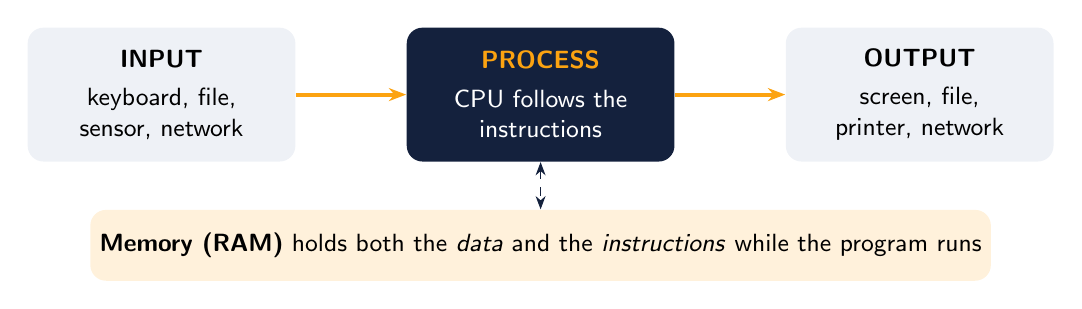
\begin{tikzpicture}[node distance=14mm,
  blk/.style={draw=none,rounded corners=2mm,minimum width=34mm,minimum height=17mm,align=center,font=\sffamily\small}]
\node[blk,fill=mist] (i) {\textbf{INPUT}\\[1mm] keyboard, file,\\ sensor, network};
\node[blk,fill=ink,text=white,right=of i] (p) {\textbf{\color{amber}PROCESS}\\[1mm] CPU follows the\\ instructions};
\node[blk,fill=mist,right=of p] (o) {\textbf{OUTPUT}\\[1mm] screen, file,\\ printer, network};
\draw[arr,draw=amber,line width=1.4pt] (i)--(p); \draw[arr,draw=amber,line width=1.4pt] (p)--(o);
\node[blk,fill=amber!15,below=6mm of p,minimum width=112mm,minimum height=9mm] (m) {\textbf{Memory (RAM)} holds both the \emph{data} and the \emph{instructions} while the program runs};
\draw[<->,>=Stealth,draw=ink,dashed] (p)--(m);
\end{tikzpicture}
\caption{The input--process--output model and the stored-program (von Neumann) idea.}\label{fig:ipo}
\end{figure}

The idea that the program's instructions are stored in the same memory as its data is due to John von Neumann (1945) and is still the architecture of every laptop and phone. RAM is \emph{volatile}: when the power is off it is empty, whereas files on a disk or SSD remain.

\subsection{Fast, but completely literal}
A single modern processor core executes on the order of $10^{9}$ simple instructions per second. Yet every one of those instructions belongs to only four families:
\begin{enumerate}[leftmargin=*,itemsep=1pt]
  \item \textbf{arithmetic} (add, subtract, multiply, divide),
  \item \textbf{comparison and logic} (is $a<b$? AND, OR, NOT),
  \item \textbf{data movement} (copy a value from memory to a register and back),
  \item \textbf{jumps} (continue at another instruction, possibly only if a condition holds).
\end{enumerate}
The computer never guesses what you \emph{meant}. It does exactly what it is told, in exactly the order it is told. Consequently:

\begin{defbox}[Key insight]
The difficult part of programming is not typing code. It is deciding the exact, unambiguous sequence of steps that solves the problem, the \textbf{algorithm}. The programming language only writes those steps in a form the machine can execute.
\end{defbox}

\subsection{From an idea to a running program}
Figure~\ref{fig:pipeline} shows what happens to your work. You write the first two boxes; the tools do the rest when you type \texttt{dotnet run}.

\begin{figure}[h]\centering
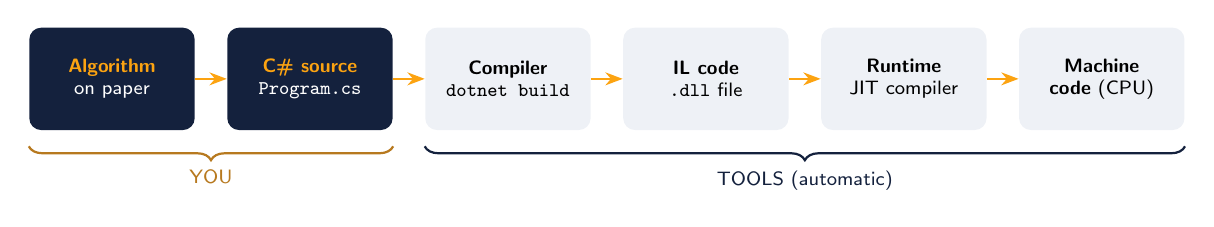
\begin{tikzpicture}[node distance=4mm,
  st/.style={rounded corners=1.5mm,minimum width=21mm,minimum height=13mm,align=center,font=\sffamily\scriptsize}]
\node[st,fill=ink,text=white] (a) {\textbf{\color{amber}Algorithm}\\ on paper};
\node[st,fill=ink,text=white,right=of a] (b) {\textbf{\color{amber}C\# source}\\ \texttt{Program.cs}};
\node[st,fill=mist,right=of b] (c) {\textbf{Compiler}\\ \texttt{dotnet build}};
\node[st,fill=mist,right=of c] (d) {\textbf{IL code}\\ \texttt{.dll} file};
\node[st,fill=mist,right=of d] (e) {\textbf{Runtime}\\ JIT compiler};
\node[st,fill=mist,right=of e] (f) {\textbf{Machine}\\ \textbf{code} (CPU)};
\foreach \x/\y in {a/b,b/c,c/d,d/e,e/f} \draw[arr,draw=amber] (\x)--(\y);
\draw[decorate,decoration={brace,mirror,amplitude=5pt},thick,amberdk] ([yshift=-2mm]a.south west)--([yshift=-2mm]b.south east) node[midway,below=5pt,font=\sffamily\scriptsize,amberdk]{YOU};
\draw[decorate,decoration={brace,mirror,amplitude=5pt},thick,ink] ([yshift=-2mm]c.south west)--([yshift=-2mm]f.south east) node[midway,below=5pt,font=\sffamily\scriptsize,ink]{TOOLS (automatic)};
\end{tikzpicture}
\caption{The C\# tool chain. IL = Intermediate Language; JIT = just-in-time compilation.}\label{fig:pipeline}
\end{figure}

The C\# compiler (called Roslyn) translates source code into \term{Intermediate Language} (IL), stored in a \texttt{.dll} file. When the program starts, the .NET runtime translates the IL into machine code for the actual processor (x64, ARM64, \dots). This is why the same compiled program runs on Windows, Linux and macOS.

\begin{table}[h]\centering\small
\begin{tabularx}{\linewidth}{lp{42mm}L}
\toprule
Level & Example: ``put 5 in a register, add 3'' & Characteristics\\ \midrule
Machine code (x86, hex) & \texttt{B8 05 00 00 00}\newline\texttt{83 C0 03} & The bytes the CPU actually reads. Practically unreadable for humans.\\
Assembly & \texttt{mov eax, 5}\newline\texttt{add eax, 3} & One mnemonic per machine instruction; tied to one processor family.\\
High-level (C\#) & \texttt{int sum = 5 + 3;} & Close to human thinking; portable across systems.\\ \bottomrule
\end{tabularx}
\caption{The same computation at three levels of abstraction.}
\end{table}

\begin{activity}[Think about it]
For each of the following, name the input, the process and the output: a pocket calculator; an ATM withdrawal; a navigation app computing a route; a thermostat.
\end{activity}

% =====================================================================
\section{What is an algorithm?}\label{sec:algorithm}

\subsection{The Exact Instructions Challenge}
In class we watch a short video in which children write instructions for making a sandwich, and their father follows them \emph{literally}: ``put the peanut butter on the bread'' results in the closed jar being placed on the loaf. While watching, note down (i)~which instruction was ambiguous, (ii)~which step was missing, (iii)~which step was in the wrong order, (iv)~whether the ``algorithm'' ever ended, and (v)~how the children fixed it. The father behaves exactly like a processor, and the children's cycle of \emph{write, test, fail, fix} is exactly how programs are developed.

\subsection{Definition}
\begin{defbox}[Definition -- Algorithm]
An \textbf{algorithm} is a \textcolor{amber}{\textbf{finite}} sequence of \textcolor{amber}{\textbf{well-defined}} steps that transforms a given \textcolor{amber}{\textbf{input}} into the desired \textcolor{amber}{\textbf{output}}, and then stops.
\end{defbox}

\paragraph{Where the word comes from.} Muhammad ibn Mūsā al-Khwārizmī (c.\,780--850) worked at the House of Wisdom in Baghdad. His book on calculating with Hindu--Arabic numerals introduced the decimal system to Europe, where his name was Latinised as \emph{Algoritmi}; hence \emph{algorithm}. The title of his other book, \emph{al-Jabr}, gave us the word \emph{algebra}.

\paragraph{Algorithm versus program.} An algorithm is an \emph{idea}, independent of any language; it can be written in words, in pseudocode or as a flowchart. A \term{program} is one \emph{implementation} of that idea in a particular programming language. One algorithm can be implemented in C\#, Python, Java or any other language: the relation is one-to-many. A recipe is an algorithm; the dish cooked in a particular kitchen is a program run.

\subsection{The five properties of an algorithm}
Following D.\,E.~Knuth, a procedure qualifies as an algorithm only if it has all five properties below.

\begin{center}\small
\begin{tabularx}{\linewidth}{>{\bfseries}p{27mm}L>{\leavevmode\itshape\color{errc}}p{47mm}}
\hrow \hdr{Property} & \hdr{Meaning} & \hdr{Violated by \dots}\\
Finiteness & It stops after a finite number of steps. & ``Keep stirring.'' (until when?)\\
\rowcolor{mist} Definiteness & Every step is precise and unambiguous. & ``Add some sugar.'' (how much?)\\
Input & It has zero or more clearly specified inputs. & ``Take the bread.'' (which bread?)\\
\rowcolor{mist} Output & It produces at least one result related to the input. & An empty plate.\\
Effectiveness & Every step is basic enough to be carried out exactly. & ``Make it tasty.''\\
\end{tabularx}
\end{center}

For practical programming we add a sixth requirement: \term{correctness}. The algorithm must produce the right output for \emph{every} valid input, including unusual ones (the \emph{edge cases}).

\subsection{Quiz: algorithm or not?}
Decide for each item whether it is an algorithm. If not, name the property that fails.
\begin{enumerate}[leftmargin=*,itemsep=1pt]
  \item The instructions on a shampoo bottle: ``Lather. Rinse. Repeat.''
  \item The long-division method you learned in primary school.
  \item ``Print the largest prime number.''
  \item A recipe step: ``Add salt to taste.''
  \item Finding a word in a paper dictionary by opening it near the word's first letter and moving forwards or backwards.
  \item ``Choose the best football team in the world.''
\end{enumerate}
\begin{notebox}[Answers]
(1)~No: it never stops (finiteness). (2)~Yes. (3)~No: Euclid proved that there are infinitely many primes, so no largest one exists; the procedure never finishes and produces no output. (4)~No: ``to taste'' is not precise (definiteness). (5)~Yes: the dictionary is finite and alphabetically ordered, so the search always ends. This is the idea behind \emph{binary search} (Week~10). (6)~No: there is no agreed criterion (definiteness, effectiveness).
\end{notebox}

\subsection{An everyday algorithm: brewing Turkish tea}
Compare the vague version ``boil water, add tea, serve'' with the precise version below. The colours mark the three kinds of structure discussed in the next subsection.

\begin{pseudobox}[Algorithm 1 -- Brewing Turkish tea]
\begin{enumerate}[leftmargin=*,itemsep=0pt]
  \item Fill the kettle (bottom pot) with 1\,L of water.
  \item Put 4 teaspoons of black tea into the teapot (top pot).
  \item Place the teapot on the kettle and turn the stove on.
  \item \textcolor{repc}{\textbf{WHILE} the water is not boiling: wait 1 minute.}
  \item Pour boiling water into the teapot until it is $\tfrac34$ full.
  \item Lower the heat and wait 15 minutes.
  \item \textcolor{selc}{\textbf{IF} the guest wants strong tea \textbf{THEN} fill the glass $\tfrac23$ with tea, \textbf{ELSE} fill it $\tfrac13$ with tea.}
  \item Top up the glass with hot water. \textbf{STOP}.
\end{enumerate}
\end{pseudobox}

\subsection{Three structures are enough}
Every algorithm can be built from only three control structures. This is the \term{structured program theorem} of B\"ohm and Jacopini (1966).

\begin{center}\small
\begin{tabularx}{\linewidth}{>{\bfseries}p{24mm}L>{\raggedright\arraybackslash}p{44mm}c}
\hrow \hdr{Structure} & \hdr{Meaning} & \hdr{Pseudocode example} & \hdr{C\# in}\\
\textcolor{seqc}{Sequence} & Steps executed one after another, top to bottom. & \READ $a$, $b$\newline $s\gets a+b$\newline \PRINT $s$ & Weeks 3--4\\
\rowcolor{mist}\textcolor{selc}{Selection} & Choose between paths according to a condition. & \textbf{IF} $age\ge 18$ \textbf{THEN}\newline\hspace*{3mm}\PRINT\str{adult}\newline\textbf{ELSE} \PRINT\str{minor} & Week 5\\
\textcolor{repc}{Repetition} & Repeat a block while a condition holds. & \textbf{WHILE} $i\le 10$\newline\hspace*{3mm}\PRINT $i$;\ $i\gets i+1$ & Weeks 6--7\\
\end{tabularx}
\end{center}
This theorem is why the course is ordered the way it is: after sequence, selection and repetition you have, in principle, everything needed to express any computation.

\subsection{Four ways to write an algorithm}
The same algorithm, ``read a number and print its absolute value'', can be written in four ways:

\begin{center}
\begin{minipage}[t]{0.47\linewidth}
\textbf{(a) Natural language.} \emph{Read the number. If it is negative, remove its minus sign. Show the number.}\\[1mm]
{\small Easy for anyone to read, but often ambiguous.}

\medskip
\textbf{(b) Pseudocode.}\vspace{-2mm}
\begin{pseudobox}
\begin{algorithmic}[1]
\START
\State \READ $x$
\IfX{$x<0$}
  \State $x \gets -x$
\EndIfX
\State \PRINT $x$
\STOP
\end{algorithmic}
\end{pseudobox}
{\small Precise and needs no tools; our main notation on paper.}
\end{minipage}\hfill
\begin{minipage}[t]{0.47\linewidth}
\textbf{(c) Flowchart} (Week~2).\\[1mm]
\centering
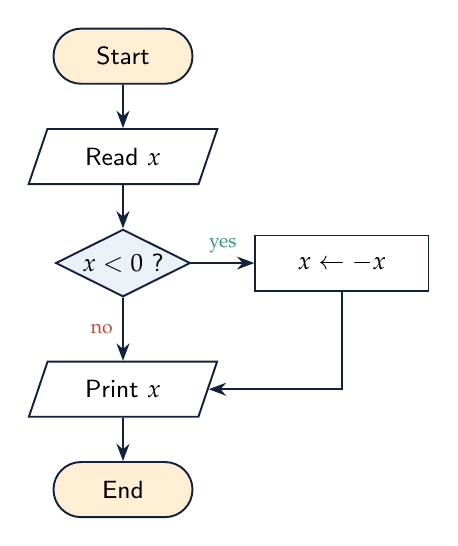
\begin{tikzpicture}[node distance=5.5mm]
\node[term] (s) {Start};
\node[io,below=of s] (r) {Read $x$};
\node[dec,below=of r] (d) {$x<0$ ?};
\node[proc,right=8mm of d] (n) {$x \gets -x$};
\node[io,below=8mm of d] (p) {Print $x$};
\node[term,below=of p] (e) {End};
\draw[arr] (s)--(r); \draw[arr] (r)--(d);
\draw[arr] (d)--node[above,font=\scriptsize,repc]{yes}(n);
\draw[arr] (d)--node[left,font=\scriptsize,errc]{no}(p);
\draw[arr] (n)|-(p);
\draw[arr] (p)--(e);
\end{tikzpicture}
\end{minipage}
\end{center}

\needspace{8\baselineskip}
\textbf{(d) C\# code} (Week~3 onwards). Executable, but with strict syntax:
\begin{lstlisting}
int x = int.Parse(Console.ReadLine());
if (x < 0)
    x = -x;
Console.WriteLine(x);
\end{lstlisting}

\subsection{Pseudocode conventions for MCMP113}\label{sec:conventions}
There is no single standard pseudocode. In this course, in all slides, homework and exams, we use the following conventions.

\begin{center}\small
\begin{tabularx}{\linewidth}{>{\ttfamily\bfseries}p{47mm}Lp{44mm}}
\hrow \hdr{Keyword} & \hdr{Meaning} & \hdr{Example}\\
START \dots\ END & beginning and end of the algorithm & \\
\rowcolor{mist} READ x & input: get a value from the user & \READ $age$\\
PRINT \dots & output: show a value or a message & \PRINT \str{Total:}, $sum$\\
\rowcolor{mist} x $\gets$ expression & assignment: evaluate the right-hand side, store it in $x$ & $total \gets total + price$\\
IF c THEN \dots\ ELSE \dots\ END IF & selection & \textbf{IF} $age\ge 18$ \textbf{THEN} \dots\\
\rowcolor{mist} WHILE c \dots\ END WHILE & repeat while condition $c$ is true & \textbf{WHILE} $i \le N$\\
FOR i $\gets$ a TO b \dots\ END FOR & repeat for $i=a,a+1,\dots,b$ & \textbf{FOR} $i\gets 1$ \textbf{TO} $10$\\
\rowcolor{mist} + \ $-$ \ $\times$ \ / \ mod & arithmetic; \texttt{mod} is the remainder & $17 \MOD 5 = 2$\\
= \ $\neq$ \ < \ $\le$ \ > \ $\ge$ & comparison (result: true or false) & \textbf{IF} $x\ne 0$ \textbf{THEN} \dots\\
\rowcolor{mist} AND \ OR \ NOT & combine conditions & \textbf{IF} $a>0$ \AND $b>0$\\
\end{tabularx}
\end{center}

\begin{warnbox}[The number-one beginner trap: assignment is not equality]
In pseudocode, $\gets$ \emph{assigns} and $=$ \emph{compares}. In C\#, \texttt{=} assigns and \texttt{==} compares. The statement $x \gets x+1$ is not an equation (as an equation, $x=x+1$ has no solution). It means ``the new value of $x$ is the old value of $x$ plus one''.
\end{warnbox}

% =====================================================================
\section{Problem-solving steps}\label{sec:problem}

\subsection{The five-step method}
Inspired by G.~P\'olya's \emph{How to Solve It} (1945), we solve every programming problem in five steps:
\begin{enumerate}[leftmargin=*,itemsep=2pt]
  \item \term{Understand (analyse).} What is given (input)? What is asked (output)? What are the constraints? Which unusual inputs can occur?
  \item \term{Design.} Write the algorithm: numbered steps, then pseudocode and/or a flowchart.
  \item \term{Implement.} Translate the algorithm into C\#.
  \item \term{Test and debug.} Run the program (or trace the algorithm by hand) with normal, boundary and invalid inputs.
  \item \term{Document.} Comments, meaningful names, notes for other people and for your future self.
\end{enumerate}
The method is a \emph{cycle}, not a straight line: a failed test sends you back to Design, or even to Understand. Beginners tend to spend most of their time in step~3; experienced programmers spend most of it in steps~1--2, which is why their step~4 is short.

\begin{notebox}[Rule of thumb]
Do not start coding until you can explain your algorithm in your own words to a classmate.
\end{notebox}

\subsection{Worked example 1: average of three exam grades}
\textbf{Problem.} A student enters three exam grades (0--100). Show the average and whether the student passed (average at least 50).

\subsubsection{Step 1 -- Understand: the IPO table}
\begin{center}\small
\begin{tabularx}{\linewidth}{LLL}
\hrow \hdr{Input} & \hdr{Process} & \hdr{Output}\\
$g_1, g_2, g_3$ (numbers, $0$--$100$) & $avg \gets (g_1+g_2+g_3)/3$; compare $avg$ with $50$ & $avg$; \str{PASSED} or \str{FAILED}\\ \bottomrule
\end{tabularx}
\end{center}
Questions to ask \emph{before} designing:
\begin{itemize}[leftmargin=*,itemsep=0pt]
  \item Can a grade be $72.5$, or only whole numbers? (This decides the data type in Week~3.)
  \item What if the user types $120$ or $-5$? (Needs a range check, i.e.\ selection, Week~5.)
  \item Is exactly $50$ a pass? (Decides between $\ge$ and $>$.)
  \item Do all exams have equal weight? (If not, a weighted average is needed.)
\end{itemize}

\subsubsection{Step 2 -- Design}
In plain language: (1) start; (2) read the three grades; (3) add them and divide by 3; (4) show the average; (5) if the average is at least 50 show ``PASSED'', otherwise ``FAILED''; (6) stop. In pseudocode:

\begin{pseudobox}[Algorithm 2 -- Average of three grades]
\begin{algorithmic}[1]
\START
\State \READ $g_1, g_2, g_3$
\State $avg \gets (g_1 + g_2 + g_3)/3$
\State \PRINT $avg$
\IfX{$avg \ge 50$}
  \State \PRINT \str{PASSED}
\ElseX
  \State \PRINT \str{FAILED}
\EndIfX
\STOP
\end{algorithmic}
\end{pseudobox}

\begin{warnbox}[Parentheses matter]
Writing $g_1 + g_2 + g_3/3$ is a different algorithm: division is performed before addition, so it computes $g_1+g_2+\frac{g_3}{3}$. For $60, 70, 80$ the correct average is $70$, whereas the wrong formula gives $156.67$. Operator precedence is studied in Week~4.
\end{warnbox}

\subsubsection{Step 4 -- Test: choosing good test cases}
Testing with a single ``nice'' input proves very little. Choose tests that are most likely to break the algorithm:
\begin{center}\small
\begin{tabularx}{\linewidth}{>{\bfseries}p{27mm}p{28mm}L}
\hrow \hdr{Kind of test} & \hdr{$g_1,g_2,g_3$} & \hdr{Expected result}\\
Normal & $60, 70, 80$ & $70.00$ -- PASSED\\
\rowcolor{mist} Boundary & $50, 50, 50$ & $50.00$ -- PASSED\\
Just below & $49, 50, 50$ & $49.67$ -- FAILED \quad ($149/3 = 49.\overline{6}$)\\
\rowcolor{mist} Maximum & $100, 100, 100$ & $100.00$ -- PASSED\\
Minimum & $0, 0, 0$ & $0.00$ -- FAILED\\
\rowcolor{mist} Out of range & $120, 70, 80$ & \textcolor{errc}{should be rejected, but Algorithm~2 prints $90.00$}\\
Wrong type & \texttt{abc}, $70$, $80$ & \textcolor{errc}{a C\# program would crash (\texttt{FormatException})}\\
\end{tabularx}
\end{center}
Boundary tests catch the most errors (for example, writing $avg>50$ instead of $avg\ge50$). The last two rows reveal \emph{missing requirements}: Algorithm~2 does not validate its input. As Dijkstra put it: \emph{``Program testing can be used to show the presence of bugs, but never to show their absence.''}

\subsection{Worked example 2: the sum $1+2+\dots+N$ and trace tables}
\begin{pseudobox}[Algorithm 3 -- Sum of the first $N$ positive integers]
\begin{algorithmic}[1]
\START
\State \READ $N$
\State $sum \gets 0$
\State $i \gets 1$
\WhileX{$i \le N$}
  \State $sum \gets sum + i$
  \State $i \gets i + 1$
\EndWhileX
\State \PRINT $sum$
\STOP
\end{algorithmic}
\end{pseudobox}

A \term{trace table} (also called a \emph{desk check}) executes the algorithm by hand: one column per variable, one row per pass through the loop. For $N=5$:
\begin{center}\small
\begin{tabular}{cccc}
\toprule
pass & $i$ (before test) & $i\le N$? & $sum$ (after pass)\\ \midrule
start & 1 & -- & 0\\
1 & 1 & yes & 1\\
2 & 2 & yes & 3\\
3 & 3 & yes & 6\\
4 & 4 & yes & 10\\
5 & 5 & yes & 15\\
exit & 6 & \textcolor{errc}{no} & \textbf{15}\\ \bottomrule
\end{tabular}
\end{center}
\textbf{Checks.} \emph{Termination:} $i$ increases by one in every pass, so it eventually exceeds $N$. \emph{Edge cases:} for $N=0$ the loop body never runs and the output is $0$, which is correct; for negative $N$ the output is also $0$ -- is that what the user expects?

\paragraph{A different algorithm for the same problem.} The young Gauss is said to have noticed that pairing the first and last terms gives $N+1$ each time:
\begin{equation}
S = \sum_{i=1}^{N} i, \qquad 2S = \underbrace{(1+N) + (2+(N-1)) + \dots + (N+1)}_{N \text{ pairs, each equal to } N+1} = N(N+1)
\quad\Longrightarrow\quad S = \frac{N(N+1)}{2}.
\end{equation}
For $N=5$: $S = 5\cdot 6/2 = 15$. Algorithm~3 needs $N$ loop passes, the formula needs one multiplication and one division, whatever $N$ is. For $N=10^{9}$ the difference is dramatic. \emph{Choosing the better algorithm is a design decision, not a coding one.}

\subsection{Worked example 3: guess my number -- efficiency}
I think of an integer between $1$ and $1000$; you guess, and I answer ``higher'', ``lower'' or ``correct''.
\begin{itemize}[leftmargin=*,itemsep=0pt]
  \item \textbf{Strategy A (linear):} guess $1, 2, 3, \dots$. Worst case: $1000$ guesses.
  \item \textbf{Strategy B (halving):} always guess the middle of the remaining range. Every answer halves the range, so after $k$ guesses at most $\lfloor 1000/2^{k}\rfloor$ candidates remain. The worst case is
  \begin{equation}
  k_{\max} = \lceil \log_2 (N+1) \rceil, \qquad N = 1000 \;\Rightarrow\; k_{\max} = 10, \quad\text{since } 2^{10}=1024 \ge 1001 .
  \end{equation}
\end{itemize}

\begin{pseudobox}[Algorithm 4 -- Guessing by halving]
\begin{algorithmic}[1]
\START
\State $low \gets 1$;\ \ $high \gets 1000$;\ \ $found \gets$ false
\WhileX{\NOT $found$}
  \State $guess \gets \lfloor (low + high)/2 \rfloor$
  \State \PRINT $guess$;\ \ \READ $answer$
  \IfX{$answer = \str{correct}$}
    \State $found \gets$ true
  \ElseX
    \IfX{$answer = \str{higher}$}
      \State $low \gets guess + 1$
    \ElseX
      \State $high \gets guess - 1$
    \EndIfX
  \EndIfX
\EndWhileX
\STOP
\end{algorithmic}
\end{pseudobox}

Trace for the secret number $737$ (10 guesses):
\begin{center}\small
\begin{tabular}{c*{10}{c}}
\toprule
guess no. & 1 & 2 & 3 & 4 & 5 & 6 & 7 & 8 & 9 & 10\\ \midrule
guess & 500 & 750 & 625 & 687 & 718 & 734 & 742 & 738 & 736 & \textbf{737}\\
answer & $\uparrow$ & $\downarrow$ & $\uparrow$ & $\uparrow$ & $\uparrow$ & $\uparrow$ & $\downarrow$ & $\downarrow$ & $\uparrow$ & \textcolor{repc}{\checkmark}\\ \bottomrule
\end{tabular}
\end{center}

\begin{center}\small
\begin{tabular}{lrrrr}
\toprule
Range size $N$ & $100$ & $1\,000$ & $10^{6}$ & $10^{9}$\\ \midrule
Strategy A, worst case & $100$ & $1\,000$ & $1\,000\,000$ & $1\,000\,000\,000$\\
Strategy B, worst case & $7$ & $10$ & $20$ & $30$\\ \bottomrule
\end{tabular}
\end{center}
Strategy A takes time proportional to $N$ (we write $O(N)$); strategy B takes time proportional to $\log_2 N$ ($O(\log N)$). Strategy B is \term{binary search}, which we implement on arrays in Week~10.

\subsection{Worked example 4: Euclid's greatest common divisor}
Written down around 300\,BC in Euclid's \emph{Elements}, this is one of the oldest non-trivial algorithms still in use; it is part of the arithmetic behind public-key cryptography (RSA) used in secure HTTPS connections.

\begin{pseudobox}[Algorithm 5 -- Euclid's GCD]
\begin{algorithmic}[1]
\START
\State \READ $a, b$ \Comment{positive integers}
\WhileX{$b \ne 0$}
  \State $r \gets a \MOD b$
  \State $a \gets b$
  \State $b \gets r$
\EndWhileX
\State \PRINT $a$
\STOP
\end{algorithmic}
\end{pseudobox}

\begin{center}\small
\begin{tabular}{ccc}
\toprule
$a$ & $b$ & $r = a \MOD b$\\ \midrule
48 & 18 & 12\\
18 & 12 & 6\\
12 & 6 & 0\\
\textcolor{repc}{\textbf{6}} & \textcolor{repc}{0} & stop: $\gcd(48,18)=6$\\ \bottomrule
\end{tabular}
\end{center}
\textbf{Why it is correct.} Any common divisor of $a$ and $b$ also divides $r=a-qb$, and any common divisor of $b$ and $r$ also divides $a=qb+r$; hence $\gcd(a,b)=\gcd(b,\,a \MOD b)$. \textbf{Why it terminates.} Since $0 \le r < b$, the value of $b$ strictly decreases in every pass and, being a non-negative integer, must reach $0$. If the input has $a<b$, the first pass simply swaps them: for $(18,48)$ we get $r=18$, $a=48$, $b=18$.

\subsection{Worked example 5: an algorithm in your wallet -- T.C. Kimlik No}
The 11-digit Turkish identity number $d_1d_2\dots d_{11}$ contains two \emph{check digits}. The rules are:
\begin{align}
& d_1 \neq 0, \\
& d_{10} = \Big( 7\,(d_1+d_3+d_5+d_7+d_9) - (d_2+d_4+d_6+d_8) \Big) \MOD 10, \\
& d_{11} = \Big( d_1 + d_2 + \dots + d_{10} \Big) \MOD 10 .
\end{align}
\textbf{Worked example} with the \emph{made-up} first nine digits $1\,2\,3\,4\,5\,6\,7\,8\,9$: the odd-position sum is $25$, the even-position sum is $20$, so $d_{10} = (175-20) \MOD 10 = 155 \MOD 10 = 5$, and $d_{11}=(45+5)\MOD 10 = 0$. The full number is $12345678950$. It passes the check but belongs to nobody.

\textbf{Why it is useful.} If exactly one of $d_1,\dots,d_{10}$ is mistyped, the sum $d_1+\dots+d_{10}$ changes by a non-zero amount between $-9$ and $+9$, so its remainder modulo~10 no longer equals $d_{11}$. The error is detected instantly, without contacting any database. The same idea protects IBANs (mod~97), EAN-13 product barcodes and credit-card numbers (the Luhn algorithm).

\begin{notebox}[Looking ahead to Week 4]
The expression $7\cdot(\text{odd sum}) - (\text{even sum})$ can be negative (e.g.\ $7\cdot 1 - 36 = -29$). Mathematically $-29 \MOD 10 = 1$, but the C\# operator \texttt{\%} gives $-29 \,\%\, 10 = -9$. A correct C\# version must use \texttt{((x \% 10) + 10) \% 10}.
\end{notebox}

\subsection{Common mistakes: bad algorithm, good algorithm}
\begin{center}\small
\begin{tabularx}{\linewidth}{>{\bfseries\raggedright\arraybackslash}p{30mm}>{\raggedright\arraybackslash\leavevmode\color{errc}}p{46mm}>{\raggedright\arraybackslash\leavevmode\color{repc!80!black}}L}
\hrow \hdr{Problem} & \hdr{Bad} & \hdr{Good}\\
Ambiguous step & ``Divide the numbers.'' & $avg \gets (g_1+g_2+g_3)/3$\\
\rowcolor{mist} No termination & ``Keep asking for a password.'' & Ask at most 3 times, then lock the account.\\
Missing edge case & $result \gets a/b$ & \textbf{IF} $b=0$ \textbf{THEN} \PRINT\str{error} \textbf{ELSE} $result\gets a/b$\\
\rowcolor{mist} Wrong order & \PRINT $sum$, then $sum \gets a+b$ & $sum \gets a+b$, then \PRINT $sum$\\
Undefined input & ``Read the grade.'' & Read a grade in $[0,100]$; reject other values.\\
\end{tabularx}
\end{center}
Each row violates one property: definiteness, finiteness, correctness, sequence and input specification, respectively.

\subsection{Sneak peek: the same algorithm in C\#}
In Week~3 you will write Algorithm~2 as follows. You do not need to understand the syntax yet; notice only that every pseudocode line maps to one or two lines of code.
\begin{lstlisting}
Console.Write("Grade 1: ");
double g1 = double.Parse(Console.ReadLine());
Console.Write("Grade 2: ");
double g2 = double.Parse(Console.ReadLine());
Console.Write("Grade 3: ");
double g3 = double.Parse(Console.ReadLine());

double avg = (g1 + g2 + g3) / 3;          // parentheses!
Console.WriteLine($"Average: {avg:F2}");

if (avg >= 50)
    Console.WriteLine("PASSED");
else
    Console.WriteLine("FAILED");
\end{lstlisting}
\begin{center}\small
\begin{tabular}{ll}
\toprule
Pseudocode & C\#\\ \midrule
\READ $x$ & \texttt{Console.ReadLine()} (plus a conversion such as \texttt{double.Parse})\\
\PRINT $x$ & \texttt{Console.WriteLine(x)}\\
$x \gets e$ & \texttt{x = e;}\\
\textbf{IF} $c$ \textbf{THEN} \dots\ \textbf{ELSE} \dots & \texttt{if (c) \{ \dots \} else \{ \dots \}}\\ \bottomrule
\end{tabular}
\end{center}
\begin{notebox}[Turkish-locale computers]
On a computer set to Turkish regional settings, \texttt{double.Parse} expects a decimal \emph{comma} ($72{,}5$), not a point. We will handle this properly in Week~3.
\end{notebox}

% =====================================================================
\needspace{12\baselineskip}
\section{Summary}\label{sec:summary}
\begin{enumerate}[leftmargin=*,itemsep=1pt]
  \item An \term{algorithm} is a finite, precise recipe that turns input into output and stops.
  \item Its five properties are finiteness, definiteness, input, output and effectiveness; in practice we also require correctness.
  \item Every algorithm is built from \textcolor{seqc}{\textbf{sequence}}, \textcolor{selc}{\textbf{selection}} and \textcolor{repc}{\textbf{repetition}}.
  \item Algorithms can be written in natural language, pseudocode, flowcharts or code.
  \item Solve problems in five steps: understand, design, implement, test, document, and loop back when a test fails.
  \item Trace tables and well-chosen test cases (normal, boundary, invalid) find errors before the computer does.
  \item Different algorithms for the same problem can differ enormously in efficiency (sum formula; binary search).
\end{enumerate}

\subsection*{Glossary (English -- Turkish)}
\begin{center}\small
\begin{tabular}{ll@{\hspace{10mm}}ll}
\toprule
algorithm & algoritma & input / output & girdi / çıktı\\
step & adım & assignment & atama\\
pseudocode & sözde kod & condition & koşul\\
flowchart & akış şeması & selection (decision) & seçim (karar)\\
sequence & sıralı yapı & repetition (loop) & tekrar (döngü)\\
variable & değişken & trace table & izleme tablosu\\
finiteness & sonluluk & edge / boundary case & sınır durumu\\
definiteness & belirlilik / kesinlik & remainder (mod) & kalan (mod)\\
effectiveness & etkinlik / yapılabilirlik & greatest common divisor & en büyük ortak bölen (EBOB)\\
compiler & derleyici & check digit & kontrol basamağı\\
source code & kaynak kod & efficiency & verimlilik\\
bug / debugging & hata / hata ayıklama & binary search & ikili arama\\ \bottomrule
\end{tabular}
\end{center}

% =====================================================================
\section{Exercises}\label{sec:exercises}
For every exercise: write the IPO table, the numbered steps and the pseudocode (using the conventions of Section~\ref{sec:conventions}), then trace your algorithm with at least one normal and one edge-case input. Difficulty: \stars{1} basic, \stars{2} intermediate, \stars{3} challenging.

\subsection{In-class exercises (groups of 2--3)}
\begin{enumerate}[label=\textbf{\Alph*.},leftmargin=*,itemsep=3pt]
  \item \stars{1} \textbf{Even or odd.} Read an integer; print whether it is even or odd.
  \solution{$n$ is even exactly when $n \MOD 2 = 0$.
  \begin{algorithmic}[1]
  \START \State \READ $n$
  \IfX{$n \MOD 2 = 0$} \State \PRINT \str{even} \ElseX \State \PRINT \str{odd} \EndIfX \STOP
  \end{algorithmic}
  Tests: $7\to$ odd, $10\to$ even, $0\to$ even. (For negative $n$ the C\# \texttt{\%} gives $-1$ for odd numbers, so test ``$\ne 0$'' rather than ``$=1$''.)}

  \item \stars{2} \textbf{Leap year.} Read a year; it is a leap year if it is divisible by 4 and not by 100, or if it is divisible by 400.
  \solution{
  \begin{algorithmic}[1]
  \START \State \READ $y$
  \IfX{($y \MOD 4 = 0$ \AND $y \MOD 100 \ne 0$) \OR $y \MOD 400 = 0$}
    \State \PRINT \str{leap year}
  \ElseX \State \PRINT \str{not a leap year} \EndIfX \STOP
  \end{algorithmic}
  Tests: $2024$ leap; $2023$ not; $1900$ not (divisible by 100 but not 400); $2000$ leap (divisible by 400).}

  \item \stars{2} \textbf{ATM withdrawal.} Given the account balance and a requested amount, allow the withdrawal only if the balance is sufficient and the amount is a positive multiple of 10; print the new balance or a reason for refusal.
  \solution{
  \begin{algorithmic}[1]
  \START \State \READ $balance$, $amount$
  \IfX{$amount \le 0$ \OR $amount \MOD 10 \ne 0$}
    \State \PRINT \str{invalid amount}
  \ElseX
    \IfX{$amount > balance$} \State \PRINT \str{insufficient funds}
    \ElseX \State $balance \gets balance - amount$ \State \PRINT \str{new balance:}, $balance$ \EndIfX
  \EndIfX \STOP
  \end{algorithmic}
  Tests: $(500,200)\to 300$; $(500,500)\to 0$ (boundary); $(500,510)\to$ insufficient; $(500,25)\to$ invalid; $(500,-10)\to$ invalid.}

  \item \stars{1} \textbf{Countdown.} Read $N$; print $N, N-1, \dots, 1$ and then ``Go!''.
  \solution{
  \begin{algorithmic}[1]
  \START \State \READ $N$
  \WhileX{$N \ge 1$} \State \PRINT $N$ \State $N \gets N - 1$ \EndWhileX
  \State \PRINT \str{Go!} \STOP
  \end{algorithmic}
  Trace $N=3$: prints $3,2,1$, Go!. Edge case $N=0$: prints only ``Go!''.}

  \item \stars{2} \textbf{Guess the number.} The computer holds a secret number; the user guesses repeatedly and receives ``higher'' or ``lower'' until correct. Also count the guesses.
  \solution{
  \begin{algorithmic}[1]
  \START \State $secret \gets$ a number between 1 and 100 \State $count \gets 0$ \State $guess \gets 0$
  \WhileX{$guess \ne secret$}
    \State \READ $guess$ \State $count \gets count + 1$
    \IfX{$guess < secret$} \State \PRINT \str{higher}
    \ElseX \IfX{$guess > secret$} \State \PRINT \str{lower} \EndIfX \EndIfX
  \EndWhileX
  \State \PRINT \str{correct after}, $count$, \str{guesses} \STOP
  \end{algorithmic}
  $guess$ is initialised to $0$ (outside the range) so that the loop runs at least once. In C\# this is a natural \texttt{do-while} (Week~7).}

  \item \stars{1} \textbf{Temperature conversion.} Read a temperature $C$ in degrees Celsius and print it in Fahrenheit, $F = \frac{9}{5}C + 32$.
  \solution{Sequence only: \READ $C$;\ $F \gets C \times 9/5 + 32$;\ \PRINT $F$. Tests: $0\to 32$, $100\to 212$, $-40\to -40$ (the two scales meet at $-40$).}
\end{enumerate}

\subsection{Homework (due before Week 2)}
\begin{enumerate}[label=\textbf{H\arabic*.},leftmargin=*,itemsep=3pt]
  \item Complete the two in-class exercises that your group did not do in class.
  \item \stars{1} Write an algorithm for a daily task of your choice that contains at least one \textbf{IF} and one \textbf{WHILE}.
  \item \stars{1} Trace Euclid's algorithm (Algorithm~5) for $(84, 36)$ in a table.
  \solution{$84 \MOD 36 = 12$; $36 \MOD 12 = 0$; so $\gcd(84,36)=12$ after two passes.}
  \item Install the .NET 10 SDK, VS Code and the C\# Dev Kit; run the four commands of Section~1.4 and post a screenshot of the output to the Telegram group.
\end{enumerate}

\subsection{Extra practice}
\begin{enumerate}[label=\textbf{P\arabic*.},leftmargin=*,itemsep=3pt]
  \item \stars{1} Trace Algorithm~3 for $N=3$ and for $N=0$. How many times is the loop condition tested in each case?
  \solution{$N=3$: output $6$; the condition is tested $4$ times ($i=1,2,3$ true; $i=4$ false). $N=0$: output $0$; tested once. In general the condition is tested $N+1$ times for $N\ge0$.}
  \item \stars{1} Use Gauss's formula to compute $1+2+\dots+100$ and $1+2+\dots+1000$.
  \solution{$100\cdot101/2 = 5050$; $1000\cdot1001/2 = 500\,500$.}
  \item \stars{2} What is the worst-case number of guesses with the halving strategy for a secret number between 1 and 500? Between 1 and 1\,000\,000?
  \solution{$\lceil\log_2 501\rceil = 9$ (since $2^9=512\ge501$); $\lceil\log_2 1\,000\,001\rceil = 20$ (since $2^{20}=1\,048\,576$).}
  \item \stars{2} Trace Euclid's algorithm for $(18,48)$ and for $(1071,462)$.
  \solution{$(18,48)$: rows $(18,48,18)$, $(48,18,12)$, $(18,12,6)$, $(12,6,0)$; result $6$. $(1071,462)$: rows $(1071,462,147)$, $(462,147,21)$, $(147,21,0)$; result $21$.}
  \item \stars{2} Compute the two check digits for the made-up first nine digits $2\,0\,2\,6\,1\,0\,0\,1\,5$.
  \solution{Odd positions: $2+2+1+0+5=10$; even positions: $0+6+0+1=7$. $d_{10} = (70-7)\MOD 10 = 63 \MOD 10 = 3$. $d_{11} = (17+3)\MOD 10 = 0$. Full number: $20261001530$.}
  \item \stars{2} \textbf{Find the bug.} A student wrote \quad $avg \gets g_1 + g_2 + g_3 / 3$ \quad and tested it only with $0,0,0$. Explain why the test passed and give a test that exposes the bug.
  \solution{For $0,0,0$ both formulas give $0$, so this test cannot tell them apart. Any non-zero input exposes it, e.g.\ $60,70,80$: correct $70$, buggy $156.67$. Lesson: a single ``trivial'' test is not enough.}
  \item \stars{2} \textbf{Maximum of $N$ numbers.} Read $N$ and then $N$ numbers one by one; print the largest. (Hint: keep a ``largest so far''.)
  \solution{
  \begin{algorithmic}[1]
  \START \State \READ $N$ \State \READ $x$ \State $max \gets x$ \State $i \gets 2$
  \WhileX{$i \le N$} \State \READ $x$ \IfX{$x > max$} \State $max \gets x$ \EndIfX \State $i \gets i+1$ \EndWhileX
  \State \PRINT $max$ \STOP
  \end{algorithmic}
  Initialising $max$ with the \emph{first} number (not with $0$) makes the algorithm correct also when all numbers are negative.}
  \item \stars{3} \textbf{Sum of digits.} Read a positive integer and print the sum of its digits (e.g.\ $4071 \to 12$). Use only $\MOD$, integer division and a loop.
  \solution{
  \begin{algorithmic}[1]
  \START \State \READ $n$ \State $s \gets 0$
  \WhileX{$n > 0$} \State $s \gets s + (n \MOD 10)$ \State $n \gets \lfloor n/10 \rfloor$ \EndWhileX
  \State \PRINT $s$ \STOP
  \end{algorithmic}
  Trace $4071$: $n=4071,\,s=1$; $n=407,\,s=8$; $n=40,\,s=8$; $n=4,\,s=12$; $n=0$ stop.}
  \item \stars{3} \textbf{Convert.} Rewrite the Turkish-tea algorithm (Algorithm~1) using the pseudocode conventions of Section~\ref{sec:conventions}, with variables for the water temperature and the guest's preference.
\end{enumerate}

% =====================================================================
\section*{References and further reading}
\addcontentsline{toc}{section}{References and further reading}
\begin{enumerate}[label={[\arabic*]},leftmargin=*,itemsep=1pt,font=\small]\small
  \item D.\,E. Knuth, \emph{The Art of Computer Programming, Vol.~1: Fundamental Algorithms}, 3rd ed., Addison-Wesley, 1997, Section~1.1.
  \item G. P\'olya, \emph{How to Solve It}, Princeton University Press, 1945.
  \item C. B\"ohm and G. Jacopini, ``Flow diagrams, Turing machines and languages with only two formation rules'', \emph{Communications of the ACM} 9(5), 366--371, 1966. \url{https://doi.org/10.1145/355592.365646}
  \item E.\,W. Dijkstra, ``Notes on Structured Programming'' (EWD249), 1970. \url{https://www.cs.utexas.edu/~EWD/ewd02xx/EWD249.PDF}
  \item T.\,H. Cormen, C.\,E. Leiserson, R.\,L. Rivest, C. Stein, \emph{Introduction to Algorithms}, 4th ed., MIT Press, 2022, Chapter~1.
  \item Microsoft, \emph{C\# documentation -- tutorials for beginners}. \url{https://learn.microsoft.com/en-us/dotnet/csharp/tour-of-csharp/tutorials/}
  \item Microsoft, \emph{.NET download (.NET 10)}. \url{https://dotnet.microsoft.com/en-us/download/dotnet/10.0}
\end{enumerate}

\end{document}
"
% =====================================================================
\documentclass[11pt,a4paper]{article}

% ---------- solutions switch ----------
\newif\ifsolutions
\ifdefined\withsolutions \solutionstrue \else \solutionsfalse \fi

% ---------- fonts ----------
\usepackage{amsmath,amssymb}
\usepackage[sc]{mathpazo}
\usepackage[no-math]{fontspec}
\setmainfont{texgyrepagella}[Extension=.otf,UprightFont=*-regular,BoldFont=*-bold,ItalicFont=*-italic,BoldItalicFont=*-bolditalic]
\setsansfont{texgyreheros}[Extension=.otf,UprightFont=*-regular,BoldFont=*-bold,ItalicFont=*-italic,BoldItalicFont=*-bolditalic]
\IfFontExistsTF{DejaVu Sans Mono}{\setmonofont{DejaVu Sans Mono}[Scale=0.84]}{\setmonofont{lmmono10-regular.otf}}

% ---------- layout ----------
\usepackage[a4paper,margin=2.3cm,headheight=14pt]{geometry}
\usepackage{microtype}
\usepackage{xcolor}
\usepackage{graphicx}
\usepackage{booktabs,tabularx,array,multirow,colortbl}
\usepackage{enumitem}
\usepackage{fancyhdr}
\usepackage{titlesec}
\usepackage[most]{tcolorbox}
\usepackage{listings}
\usepackage{algorithm}
\usepackage[noend]{algpseudocode}
\usepackage{tikz}
\usetikzlibrary{shapes.geometric,shapes.misc,arrows.meta,positioning,calc,fit,decorations.pathreplacing}
\usepackage{hyperref}
\usepackage{needspace}
\renewcommand{\arraystretch}{1.28}
\setlength{\parindent}{0pt}
\setlength{\parskip}{0.55em}

% ---------- colours (same as the slides) ----------
\definecolor{ink}{HTML}{14213D}
\definecolor{amber}{HTML}{FCA311}
\definecolor{amberdk}{HTML}{B7791F}
\definecolor{mist}{HTML}{EEF1F6}
\definecolor{slate}{HTML}{5B6478}
\definecolor{codebg}{HTML}{F4F6FA}
\definecolor{seqc}{HTML}{14213D}
\definecolor{selc}{HTML}{2F6FB3}
\definecolor{repc}{HTML}{2E9E6A}
\definecolor{errc}{HTML}{C8453B}
\hypersetup{colorlinks,linkcolor=ink,urlcolor=selc,citecolor=ink,
  pdftitle={MCMP113 Week 1 Lecture Notes},pdfauthor={Asst. Prof. Hasan Oguz, PhD}}

% ---------- headings ----------
\titleformat{\section}{\sffamily\Large\bfseries\color{ink}}{\color{amber}\texttt{>\_}\hspace{0.4em}\thesection}{0.6em}{}
\titleformat{\subsection}{\sffamily\large\bfseries\color{ink}}{\thesubsection}{0.6em}{}
\titleformat{\subsubsection}{\sffamily\normalsize\bfseries\color{ink}}{}{0em}{}
\titlespacing*{\section}{0pt}{1.6em}{0.6em}
\titlespacing*{\subsection}{0pt}{1.2em}{0.4em}

% ---------- header/footer ----------
\pagestyle{fancy}\fancyhf{}
\fancyhead[L]{\sffamily\small\color{slate}MCMP113 \textperiodcentered{} Introduction to Basic Algorithms and Programming}
\fancyhead[R]{\sffamily\small\color{slate}Week 1\ifsolutions{} \textperiodcentered{} \textcolor{errc}{Instructor edition}\fi}
\fancyfoot[C]{\sffamily\small\color{slate}\thepage}
\renewcommand{\headrulewidth}{0pt}

% ---------- boxes ----------
\newtcolorbox{defbox}[1][]{enhanced,breakable,colback=ink,colframe=ink,coltext=white,
  fonttitle=\sffamily\bfseries,coltitle=amber,title={#1},arc=2mm,boxrule=0pt,left=3mm,right=3mm,top=2mm,bottom=2mm}
\newtcolorbox{notebox}[1][Note]{enhanced,breakable,colback=amber!12,colframe=amber!12,
  fonttitle=\sffamily\bfseries,coltitle=amberdk,title={#1},arc=2mm,boxrule=0pt,left=3mm,right=3mm}
\newtcolorbox{warnbox}[1][Common mistake]{enhanced,breakable,colback=errc!8,colframe=errc!8,
  fonttitle=\sffamily\bfseries,coltitle=errc,title={#1},arc=2mm,boxrule=0pt,left=3mm,right=3mm}
\newtcolorbox{activity}[1][Activity]{enhanced,breakable,colback=mist,colframe=mist,
  fonttitle=\sffamily\bfseries,coltitle=ink,title={#1},arc=2mm,boxrule=0pt,left=3mm,right=3mm}
\newtcolorbox{pseudobox}[1][]{enhanced,colback=codebg,colframe=ink!25,
  fonttitle=\sffamily\small\bfseries,coltitle=ink,colbacktitle=ink!8,title={#1},arc=1.5mm,boxrule=0.4pt,left=2mm,right=2mm,top=1mm,bottom=1mm}
\newtcolorbox{solbox}[1][Solution]{enhanced,breakable,colback=repc!7,colframe=repc!60,
  fonttitle=\sffamily\bfseries,coltitle=white,colbacktitle=repc,title={#1},arc=1.5mm,boxrule=0.5pt}

% ---------- pseudocode conventions ----------
\algrenewcommand\algorithmicif{\textbf{IF}}
\algrenewcommand\algorithmicthen{\textbf{THEN}}
\algrenewcommand\algorithmicelse{\textbf{ELSE}}
\algrenewcommand\algorithmicwhile{\textbf{WHILE}}
\algrenewcommand\algorithmicdo{}
\algrenewcommand\algorithmicfor{\textbf{FOR}}
\algrenewcommand\algorithmicend{\textbf{END}}
\algrenewcommand\algorithmicreturn{\textbf{RETURN}}
\algrenewcommand\alglinenumber[1]{\footnotesize\color{slate}#1}
\newcommand{\READ}{\textbf{READ}\ }
\newcommand{\PRINT}{\textbf{PRINT}\ }
\newcommand{\START}{\State \textbf{START}}
\newcommand{\STOP}{\State \textbf{END}}
\newcommand{\TO}{\ \textbf{TO}\ }
\newcommand{\AND}{\ \textbf{AND}\ }
\newcommand{\OR}{\ \textbf{OR}\ }
\newcommand{\NOT}{\textbf{NOT}\ }
\newcommand{\MOD}{\mathbin{\mathrm{mod}}}
\newcommand{\str}[1]{\texttt{"#1"}}
% explicit END IF / END WHILE / END FOR lines (course convention)
\algdef{SE}[WHILEX]{WhileX}{EndWhileX}[1]{\algorithmicwhile\ #1}{\textbf{END WHILE}}
\algdef{SE}[IFX]{IfX}{EndIfX}[1]{\algorithmicif\ #1\ \algorithmicthen}{\textbf{END IF}}
\algdef{Ce}[ELSEX]{IFX}{ElseX}{EndIfX}{\algorithmicelse}
\algdef{SE}[FORX]{ForX}{EndForX}[1]{\algorithmicfor\ #1}{\textbf{END FOR}}

% ---------- C# listings ----------
\lstdefinelanguage{CSharp14}{language=[Sharp]C,
  morekeywords={var,string,double,int,bool,decimal,if,else,while,for,foreach,return,true,false,using,static,void,new},
  sensitive=true}
\lstset{language=CSharp14,basicstyle=\ttfamily\small,keywordstyle=\color{selc}\bfseries,
  stringstyle=\color{repc!80!black},commentstyle=\color{slate}\itshape,
  backgroundcolor=\color{codebg},frame=single,rulecolor=\color{ink!25},framesep=4pt,xleftmargin=6pt,xrightmargin=6pt,
  numbers=left,numberstyle=\scriptsize\color{slate},numbersep=8pt,showstringspaces=false,
  columns=fullflexible,keepspaces=true,upquote=true,breaklines=true,aboveskip=0.8em,belowskip=0.8em}
\lstdefinestyle{shell}{language={},numbers=none,basicstyle=\ttfamily\small\color{white},backgroundcolor=\color{ink},rulecolor=\color{ink}}

% ---------- misc ----------
\newcommand{\kw}[1]{\textsf{\bfseries #1}}
\newcommand{\term}[1]{\textbf{\color{ink}#1}}
\newcommand{\solution}[1]{\ifsolutions\begin{solbox}#1\end{solbox}\fi}
\newcolumntype{L}{>{\raggedright\arraybackslash}X}
\newcommand{\hdr}[1]{\textcolor{white}{\sffamily\bfseries #1}}
\newcommand{\hrow}{\rowcolor{ink}}
\newcommand{\stars}[1]{\textcolor{amberdk}{\ifcase#1\or$\star$\or$\star\star$\or$\star\star\star$\fi}}

\tikzset{
  fc/.style={draw=ink,line width=0.7pt,align=center,font=\sffamily\small,minimum height=7mm},
  term/.style={fc,rounded rectangle,fill=amber!18,minimum width=20mm},
  io/.style={fc,trapezium,trapezium left angle=72,trapezium right angle=108,trapezium stretches=true,fill=white,minimum width=24mm},
  proc/.style={fc,rectangle,fill=white,minimum width=22mm},
  dec/.style={fc,diamond,aspect=2,fill=selc!10,inner sep=1pt},
  arr/.style={-{Stealth[length=2.2mm]},draw=ink,line width=0.7pt},
}

% =====================================================================
\begin{document}

% ---------------- title block ----------------
\begin{tcolorbox}[enhanced,colback=ink,colframe=ink,arc=3mm,boxrule=0pt,left=6mm,right=6mm,top=5mm,bottom=5mm]
\begin{minipage}[c]{0.74\linewidth}
{\ttfamily\bfseries\color{amber}>\_ MCMP113}\\[2mm]
{\sffamily\bfseries\LARGE\color{white}Introduction to Basic Algorithms\\[1mm] and Programming}\\[3mm]
{\sffamily\large\color{white!80!ink}Week 1 Lecture Notes: Course Introduction,\\ the Concept of an Algorithm, and Problem-Solving Steps}\\[4mm]
{\sffamily\small\color{white}\textbf{Asst.\ Prof.\ Hasan Oğuz, PhD}\\
\color{white!75!ink}Istanbul Okan University \textperiodcentered{} Vocational School \textperiodcentered{} 2026--2027 Fall}
\ifsolutions\\[2mm]{\sffamily\small\bfseries\color{amber}INSTRUCTOR EDITION -- contains solutions}\fi
\end{minipage}\hfill
\begin{minipage}[c]{0.22\linewidth}\centering
\end{minipage}
\end{tcolorbox}

\vspace{2mm}
\begin{notebox}[How to use these notes]
These notes follow the Week~1 slides and add the details that do not fit on a slide: full explanations, every worked example with its trace table, a pseudocode reference card, an English--Turkish glossary and graded exercises. Week~1 is \emph{conceptual}: we do not write C\# yet. Read Sections~\ref{sec:computer}--\ref{sec:problem} before Week~2, then do the exercises in Section~\ref{sec:exercises}.
\end{notebox}

{\small\tableofcontents}

% =====================================================================
\section{About the course}\label{sec:course}

\subsection{Aims and learning outcomes}
MCMP113 teaches you to \emph{think like a programmer}: to turn a problem stated in everyday language into a precise sequence of steps, and then into a working C\# console application. By the end of the semester you should be able to:
\begin{enumerate}[leftmargin=*,itemsep=1pt]
  \item \term{Think algorithmically}: break a real problem into precise, finite, ordered steps.
  \item \term{Draw and read flowcharts}: express an algorithm visually before writing any code.
  \item \term{Write C\# console applications} using variables, operators, decisions and loops correctly.
  \item \term{Work with arrays}: store, search, sort and process collections of data.
  \item \term{Structure programs with functions} that take parameters and return values.
  \item \term{Test and debug}: trace code by hand and locate errors systematically.
\end{enumerate}
Outcomes~1--2 do not depend on any programming language. They are the real skill; C\# is the vehicle we use to practise it.

\subsection{Weekly plan}
\begin{center}\small
\begin{tabularx}{\linewidth}{>{\centering\arraybackslash}p{9mm}L>{\raggedright\arraybackslash}p{38mm}}
\hrow \hdr{Week} & \hdr{Topic} & \hdr{Preparation}\\
\rowcolor{amber!15} 1 & Course introduction \textperiodcentered{} the concept of an algorithm \textperiodcentered{} problem-solving steps & Lecture notes\\
2 & Flowcharts and their symbols \textperiodcentered{} basic flowchart examples & Lecture notes\\
\rowcolor{mist} 3 & Introduction to programming languages \textperiodcentered{} variables \textperiodcentered{} data types \textperiodcentered{} constants & Notes, sample code\\
4 & Arithmetic, logical and relational operators & Notes, sample code\\
\rowcolor{mist} 5 & Decision structures: \texttt{if-else}, \texttt{if-else if}, \texttt{switch-case} & Notes, sample code\\
6 & Loops: the \texttt{for} loop & Notes, sample code\\
\rowcolor{mist} 7 & Loops: \texttt{while} and \texttt{do-while} & Notes, sample code\\
\rowcolor{ink} \textcolor{amber}{\bfseries 8} & \textcolor{white}{\bfseries MIDTERM EXAM} & \textcolor{white}{Review weeks 1--7}\\
9 & One-dimensional arrays: declaration, assignment, element access & Notes, sample code\\
\rowcolor{mist} 10 & Array operations: searching, sorting, finding the maximum/minimum & Notes, sample code\\
11 & Multi-dimensional arrays (matrices) & Notes, sample code\\
\rowcolor{mist} 12 & Functions: definition, calling, parameter passing & Notes, sample code\\
13 & Value-returning and \texttt{void} functions \textperiodcentered{} scope & Notes, sample code\\
\rowcolor{mist} 14 & Basic file operations \textperiodcentered{} semester review & Lecture notes\\
\rowcolor{ink} \textcolor{amber}{\bfseries 15} & \textcolor{white}{\bfseries FINAL EXAM} & \textcolor{white}{Review all topics}\\
\end{tabularx}
\end{center}

\subsection{Assessment and attendance}
\begin{center}
\begin{tabular}{lcc}
\toprule
Component & Week & Weight\\ \midrule
Midterm exam & 8 & $40\%$\\
Final exam & 15 & $60\%$\\ \bottomrule
\end{tabular}
\end{center}
Both exams test \emph{reasoning}: tracing algorithms, drawing flowcharts, and writing short programs by hand. The weekly exercises are not graded, but they are the most direct preparation for the exams. Attendance follows the university regulations.

\subsection{Software (install before Week 3)}
All tools are free and run on Windows, macOS and Linux.
\begin{itemize}[leftmargin=*,itemsep=1pt]
  \item \textbf{.NET 10 SDK} (the current long-term-support release): \url{https://dotnet.microsoft.com/en-us/download/dotnet/10.0}
  \item \textbf{Visual Studio Code}: \url{https://code.visualstudio.com/}
  \item \textbf{C\# Dev Kit} extension for VS Code (search ``C\# Dev Kit'' in the Extensions panel).
\end{itemize}
Check your installation in a terminal (the exact version number may differ):
\begin{lstlisting}[style=shell]
> dotnet --version
10.0.100
> dotnet new console -n Hello
> cd Hello
> dotnet run
Hello, World!
\end{lstlisting}
\begin{notebox}[Why .NET 10 and not .NET 8?]
Support for .NET~8 ends in November 2026, in the middle of our semester; .NET~10 is supported until November 2028. Code written in this course runs on both, but install~10.
\end{notebox}

% =====================================================================
\section{How a computer solves problems}\label{sec:computer}

\subsection{Input -- Process -- Output}
Every program, from a calculator to a video game, follows the same pattern (Figure~\ref{fig:ipo}): data comes \term{in}, the processor \term{processes} it by following instructions, and results go \term{out}.

\begin{figure}[h]\centering
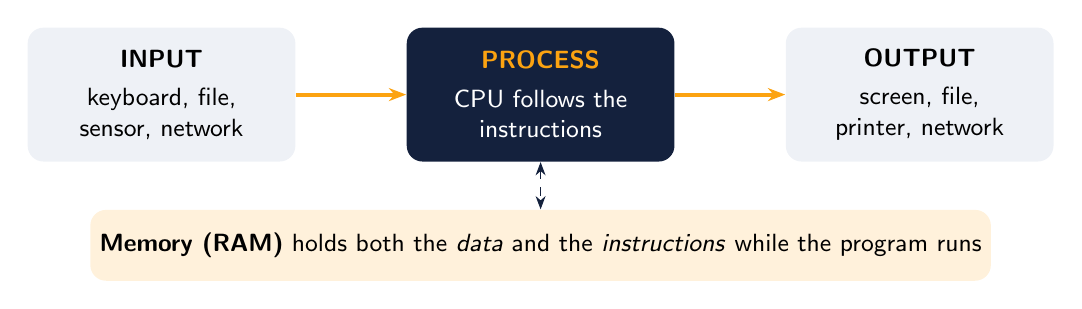
\begin{tikzpicture}[node distance=14mm,
  blk/.style={draw=none,rounded corners=2mm,minimum width=34mm,minimum height=17mm,align=center,font=\sffamily\small}]
\node[blk,fill=mist] (i) {\textbf{INPUT}\\[1mm] keyboard, file,\\ sensor, network};
\node[blk,fill=ink,text=white,right=of i] (p) {\textbf{\color{amber}PROCESS}\\[1mm] CPU follows the\\ instructions};
\node[blk,fill=mist,right=of p] (o) {\textbf{OUTPUT}\\[1mm] screen, file,\\ printer, network};
\draw[arr,draw=amber,line width=1.4pt] (i)--(p); \draw[arr,draw=amber,line width=1.4pt] (p)--(o);
\node[blk,fill=amber!15,below=6mm of p,minimum width=112mm,minimum height=9mm] (m) {\textbf{Memory (RAM)} holds both the \emph{data} and the \emph{instructions} while the program runs};
\draw[<->,>=Stealth,draw=ink,dashed] (p)--(m);
\end{tikzpicture}
\caption{The input--process--output model and the stored-program (von Neumann) idea.}\label{fig:ipo}
\end{figure}

The idea that the program's instructions are stored in the same memory as its data is due to John von Neumann (1945) and is still the architecture of every laptop and phone. RAM is \emph{volatile}: when the power is off it is empty, whereas files on a disk or SSD remain.

\subsection{Fast, but completely literal}
A single modern processor core executes on the order of $10^{9}$ simple instructions per second. Yet every one of those instructions belongs to only four families:
\begin{enumerate}[leftmargin=*,itemsep=1pt]
  \item \textbf{arithmetic} (add, subtract, multiply, divide),
  \item \textbf{comparison and logic} (is $a<b$? AND, OR, NOT),
  \item \textbf{data movement} (copy a value from memory to a register and back),
  \item \textbf{jumps} (continue at another instruction, possibly only if a condition holds).
\end{enumerate}
The computer never guesses what you \emph{meant}. It does exactly what it is told, in exactly the order it is told. Consequently:

\begin{defbox}[Key insight]
The difficult part of programming is not typing code. It is deciding the exact, unambiguous sequence of steps that solves the problem, the \textbf{algorithm}. The programming language only writes those steps in a form the machine can execute.
\end{defbox}

\subsection{From an idea to a running program}
Figure~\ref{fig:pipeline} shows what happens to your work. You write the first two boxes; the tools do the rest when you type \texttt{dotnet run}.

\begin{figure}[h]\centering
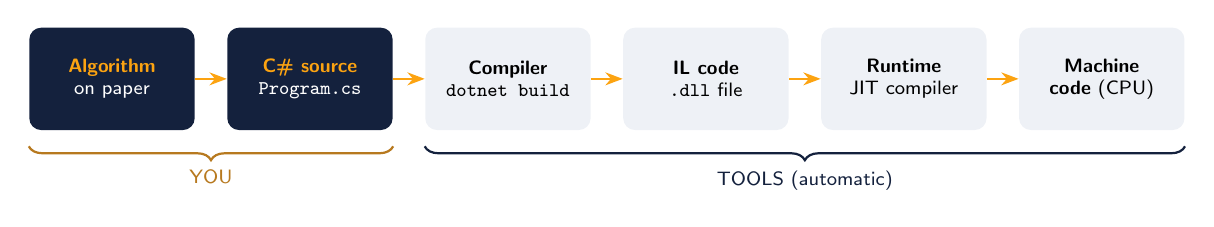
\begin{tikzpicture}[node distance=4mm,
  st/.style={rounded corners=1.5mm,minimum width=21mm,minimum height=13mm,align=center,font=\sffamily\scriptsize}]
\node[st,fill=ink,text=white] (a) {\textbf{\color{amber}Algorithm}\\ on paper};
\node[st,fill=ink,text=white,right=of a] (b) {\textbf{\color{amber}C\# source}\\ \texttt{Program.cs}};
\node[st,fill=mist,right=of b] (c) {\textbf{Compiler}\\ \texttt{dotnet build}};
\node[st,fill=mist,right=of c] (d) {\textbf{IL code}\\ \texttt{.dll} file};
\node[st,fill=mist,right=of d] (e) {\textbf{Runtime}\\ JIT compiler};
\node[st,fill=mist,right=of e] (f) {\textbf{Machine}\\ \textbf{code} (CPU)};
\foreach \x/\y in {a/b,b/c,c/d,d/e,e/f} \draw[arr,draw=amber] (\x)--(\y);
\draw[decorate,decoration={brace,mirror,amplitude=5pt},thick,amberdk] ([yshift=-2mm]a.south west)--([yshift=-2mm]b.south east) node[midway,below=5pt,font=\sffamily\scriptsize,amberdk]{YOU};
\draw[decorate,decoration={brace,mirror,amplitude=5pt},thick,ink] ([yshift=-2mm]c.south west)--([yshift=-2mm]f.south east) node[midway,below=5pt,font=\sffamily\scriptsize,ink]{TOOLS (automatic)};
\end{tikzpicture}
\caption{The C\# tool chain. IL = Intermediate Language; JIT = just-in-time compilation.}\label{fig:pipeline}
\end{figure}

The C\# compiler (called Roslyn) translates source code into \term{Intermediate Language} (IL), stored in a \texttt{.dll} file. When the program starts, the .NET runtime translates the IL into machine code for the actual processor (x64, ARM64, \dots). This is why the same compiled program runs on Windows, Linux and macOS.

\begin{table}[h]\centering\small
\begin{tabularx}{\linewidth}{lp{42mm}L}
\toprule
Level & Example: ``put 5 in a register, add 3'' & Characteristics\\ \midrule
Machine code (x86, hex) & \texttt{B8 05 00 00 00}\newline\texttt{83 C0 03} & The bytes the CPU actually reads. Practically unreadable for humans.\\
Assembly & \texttt{mov eax, 5}\newline\texttt{add eax, 3} & One mnemonic per machine instruction; tied to one processor family.\\
High-level (C\#) & \texttt{int sum = 5 + 3;} & Close to human thinking; portable across systems.\\ \bottomrule
\end{tabularx}
\caption{The same computation at three levels of abstraction.}
\end{table}

\begin{activity}[Think about it]
For each of the following, name the input, the process and the output: a pocket calculator; an ATM withdrawal; a navigation app computing a route; a thermostat.
\end{activity}

% =====================================================================
\section{What is an algorithm?}\label{sec:algorithm}

\subsection{The Exact Instructions Challenge}
In class we watch a short video in which children write instructions for making a sandwich, and their father follows them \emph{literally}: ``put the peanut butter on the bread'' results in the closed jar being placed on the loaf. While watching, note down (i)~which instruction was ambiguous, (ii)~which step was missing, (iii)~which step was in the wrong order, (iv)~whether the ``algorithm'' ever ended, and (v)~how the children fixed it. The father behaves exactly like a processor, and the children's cycle of \emph{write, test, fail, fix} is exactly how programs are developed.

\subsection{Definition}
\begin{defbox}[Definition -- Algorithm]
An \textbf{algorithm} is a \textcolor{amber}{\textbf{finite}} sequence of \textcolor{amber}{\textbf{well-defined}} steps that transforms a given \textcolor{amber}{\textbf{input}} into the desired \textcolor{amber}{\textbf{output}}, and then stops.
\end{defbox}

\paragraph{Where the word comes from.} Muhammad ibn Mūsā al-Khwārizmī (c.\,780--850) worked at the House of Wisdom in Baghdad. His book on calculating with Hindu--Arabic numerals introduced the decimal system to Europe, where his name was Latinised as \emph{Algoritmi}; hence \emph{algorithm}. The title of his other book, \emph{al-Jabr}, gave us the word \emph{algebra}.

\paragraph{Algorithm versus program.} An algorithm is an \emph{idea}, independent of any language; it can be written in words, in pseudocode or as a flowchart. A \term{program} is one \emph{implementation} of that idea in a particular programming language. One algorithm can be implemented in C\#, Python, Java or any other language: the relation is one-to-many. A recipe is an algorithm; the dish cooked in a particular kitchen is a program run.

\subsection{The five properties of an algorithm}
Following D.\,E.~Knuth, a procedure qualifies as an algorithm only if it has all five properties below.

\begin{center}\small
\begin{tabularx}{\linewidth}{>{\bfseries}p{27mm}L>{\leavevmode\itshape\color{errc}}p{47mm}}
\hrow \hdr{Property} & \hdr{Meaning} & \hdr{Violated by \dots}\\
Finiteness & It stops after a finite number of steps. & ``Keep stirring.'' (until when?)\\
\rowcolor{mist} Definiteness & Every step is precise and unambiguous. & ``Add some sugar.'' (how much?)\\
Input & It has zero or more clearly specified inputs. & ``Take the bread.'' (which bread?)\\
\rowcolor{mist} Output & It produces at least one result related to the input. & An empty plate.\\
Effectiveness & Every step is basic enough to be carried out exactly. & ``Make it tasty.''\\
\end{tabularx}
\end{center}

For practical programming we add a sixth requirement: \term{correctness}. The algorithm must produce the right output for \emph{every} valid input, including unusual ones (the \emph{edge cases}).

\subsection{Quiz: algorithm or not?}
Decide for each item whether it is an algorithm. If not, name the property that fails.
\begin{enumerate}[leftmargin=*,itemsep=1pt]
  \item The instructions on a shampoo bottle: ``Lather. Rinse. Repeat.''
  \item The long-division method you learned in primary school.
  \item ``Print the largest prime number.''
  \item A recipe step: ``Add salt to taste.''
  \item Finding a word in a paper dictionary by opening it near the word's first letter and moving forwards or backwards.
  \item ``Choose the best football team in the world.''
\end{enumerate}
\begin{notebox}[Answers]
(1)~No: it never stops (finiteness). (2)~Yes. (3)~No: Euclid proved that there are infinitely many primes, so no largest one exists; the procedure never finishes and produces no output. (4)~No: ``to taste'' is not precise (definiteness). (5)~Yes: the dictionary is finite and alphabetically ordered, so the search always ends. This is the idea behind \emph{binary search} (Week~10). (6)~No: there is no agreed criterion (definiteness, effectiveness).
\end{notebox}

\subsection{An everyday algorithm: brewing Turkish tea}
Compare the vague version ``boil water, add tea, serve'' with the precise version below. The colours mark the three kinds of structure discussed in the next subsection.

\begin{pseudobox}[Algorithm 1 -- Brewing Turkish tea]
\begin{enumerate}[leftmargin=*,itemsep=0pt]
  \item Fill the kettle (bottom pot) with 1\,L of water.
  \item Put 4 teaspoons of black tea into the teapot (top pot).
  \item Place the teapot on the kettle and turn the stove on.
  \item \textcolor{repc}{\textbf{WHILE} the water is not boiling: wait 1 minute.}
  \item Pour boiling water into the teapot until it is $\tfrac34$ full.
  \item Lower the heat and wait 15 minutes.
  \item \textcolor{selc}{\textbf{IF} the guest wants strong tea \textbf{THEN} fill the glass $\tfrac23$ with tea, \textbf{ELSE} fill it $\tfrac13$ with tea.}
  \item Top up the glass with hot water. \textbf{STOP}.
\end{enumerate}
\end{pseudobox}

\subsection{Three structures are enough}
Every algorithm can be built from only three control structures. This is the \term{structured program theorem} of B\"ohm and Jacopini (1966).

\begin{center}\small
\begin{tabularx}{\linewidth}{>{\bfseries}p{24mm}L>{\raggedright\arraybackslash}p{44mm}c}
\hrow \hdr{Structure} & \hdr{Meaning} & \hdr{Pseudocode example} & \hdr{C\# in}\\
\textcolor{seqc}{Sequence} & Steps executed one after another, top to bottom. & \READ $a$, $b$\newline $s\gets a+b$\newline \PRINT $s$ & Weeks 3--4\\
\rowcolor{mist}\textcolor{selc}{Selection} & Choose between paths according to a condition. & \textbf{IF} $age\ge 18$ \textbf{THEN}\newline\hspace*{3mm}\PRINT\str{adult}\newline\textbf{ELSE} \PRINT\str{minor} & Week 5\\
\textcolor{repc}{Repetition} & Repeat a block while a condition holds. & \textbf{WHILE} $i\le 10$\newline\hspace*{3mm}\PRINT $i$;\ $i\gets i+1$ & Weeks 6--7\\
\end{tabularx}
\end{center}
This theorem is why the course is ordered the way it is: after sequence, selection and repetition you have, in principle, everything needed to express any computation.

\subsection{Four ways to write an algorithm}
The same algorithm, ``read a number and print its absolute value'', can be written in four ways:

\begin{center}
\begin{minipage}[t]{0.47\linewidth}
\textbf{(a) Natural language.} \emph{Read the number. If it is negative, remove its minus sign. Show the number.}\\[1mm]
{\small Easy for anyone to read, but often ambiguous.}

\medskip
\textbf{(b) Pseudocode.}\vspace{-2mm}
\begin{pseudobox}
\begin{algorithmic}[1]
\START
\State \READ $x$
\IfX{$x<0$}
  \State $x \gets -x$
\EndIfX
\State \PRINT $x$
\STOP
\end{algorithmic}
\end{pseudobox}
{\small Precise and needs no tools; our main notation on paper.}
\end{minipage}\hfill
\begin{minipage}[t]{0.47\linewidth}
\textbf{(c) Flowchart} (Week~2).\\[1mm]
\centering
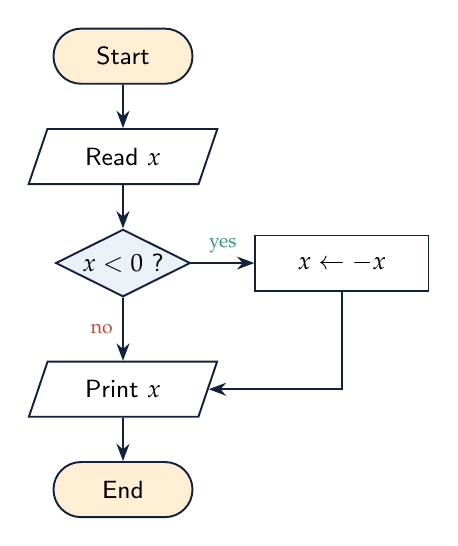
\begin{tikzpicture}[node distance=5.5mm]
\node[term] (s) {Start};
\node[io,below=of s] (r) {Read $x$};
\node[dec,below=of r] (d) {$x<0$ ?};
\node[proc,right=8mm of d] (n) {$x \gets -x$};
\node[io,below=8mm of d] (p) {Print $x$};
\node[term,below=of p] (e) {End};
\draw[arr] (s)--(r); \draw[arr] (r)--(d);
\draw[arr] (d)--node[above,font=\scriptsize,repc]{yes}(n);
\draw[arr] (d)--node[left,font=\scriptsize,errc]{no}(p);
\draw[arr] (n)|-(p);
\draw[arr] (p)--(e);
\end{tikzpicture}
\end{minipage}
\end{center}

\needspace{8\baselineskip}
\textbf{(d) C\# code} (Week~3 onwards). Executable, but with strict syntax:
\begin{lstlisting}
int x = int.Parse(Console.ReadLine());
if (x < 0)
    x = -x;
Console.WriteLine(x);
\end{lstlisting}

\subsection{Pseudocode conventions for MCMP113}\label{sec:conventions}
There is no single standard pseudocode. In this course, in all slides, homework and exams, we use the following conventions.

\begin{center}\small
\begin{tabularx}{\linewidth}{>{\ttfamily\bfseries}p{47mm}Lp{44mm}}
\hrow \hdr{Keyword} & \hdr{Meaning} & \hdr{Example}\\
START \dots\ END & beginning and end of the algorithm & \\
\rowcolor{mist} READ x & input: get a value from the user & \READ $age$\\
PRINT \dots & output: show a value or a message & \PRINT \str{Total:}, $sum$\\
\rowcolor{mist} x $\gets$ expression & assignment: evaluate the right-hand side, store it in $x$ & $total \gets total + price$\\
IF c THEN \dots\ ELSE \dots\ END IF & selection & \textbf{IF} $age\ge 18$ \textbf{THEN} \dots\\
\rowcolor{mist} WHILE c \dots\ END WHILE & repeat while condition $c$ is true & \textbf{WHILE} $i \le N$\\
FOR i $\gets$ a TO b \dots\ END FOR & repeat for $i=a,a+1,\dots,b$ & \textbf{FOR} $i\gets 1$ \textbf{TO} $10$\\
\rowcolor{mist} + \ $-$ \ $\times$ \ / \ mod & arithmetic; \texttt{mod} is the remainder & $17 \MOD 5 = 2$\\
= \ $\neq$ \ < \ $\le$ \ > \ $\ge$ & comparison (result: true or false) & \textbf{IF} $x\ne 0$ \textbf{THEN} \dots\\
\rowcolor{mist} AND \ OR \ NOT & combine conditions & \textbf{IF} $a>0$ \AND $b>0$\\
\end{tabularx}
\end{center}

\begin{warnbox}[The number-one beginner trap: assignment is not equality]
In pseudocode, $\gets$ \emph{assigns} and $=$ \emph{compares}. In C\#, \texttt{=} assigns and \texttt{==} compares. The statement $x \gets x+1$ is not an equation (as an equation, $x=x+1$ has no solution). It means ``the new value of $x$ is the old value of $x$ plus one''.
\end{warnbox}

% =====================================================================
\section{Problem-solving steps}\label{sec:problem}

\subsection{The five-step method}
Inspired by G.~P\'olya's \emph{How to Solve It} (1945), we solve every programming problem in five steps:
\begin{enumerate}[leftmargin=*,itemsep=2pt]
  \item \term{Understand (analyse).} What is given (input)? What is asked (output)? What are the constraints? Which unusual inputs can occur?
  \item \term{Design.} Write the algorithm: numbered steps, then pseudocode and/or a flowchart.
  \item \term{Implement.} Translate the algorithm into C\#.
  \item \term{Test and debug.} Run the program (or trace the algorithm by hand) with normal, boundary and invalid inputs.
  \item \term{Document.} Comments, meaningful names, notes for other people and for your future self.
\end{enumerate}
The method is a \emph{cycle}, not a straight line: a failed test sends you back to Design, or even to Understand. Beginners tend to spend most of their time in step~3; experienced programmers spend most of it in steps~1--2, which is why their step~4 is short.

\begin{notebox}[Rule of thumb]
Do not start coding until you can explain your algorithm in your own words to a classmate.
\end{notebox}

\subsection{Worked example 1: average of three exam grades}
\textbf{Problem.} A student enters three exam grades (0--100). Show the average and whether the student passed (average at least 50).

\subsubsection{Step 1 -- Understand: the IPO table}
\begin{center}\small
\begin{tabularx}{\linewidth}{LLL}
\hrow \hdr{Input} & \hdr{Process} & \hdr{Output}\\
$g_1, g_2, g_3$ (numbers, $0$--$100$) & $avg \gets (g_1+g_2+g_3)/3$; compare $avg$ with $50$ & $avg$; \str{PASSED} or \str{FAILED}\\ \bottomrule
\end{tabularx}
\end{center}
Questions to ask \emph{before} designing:
\begin{itemize}[leftmargin=*,itemsep=0pt]
  \item Can a grade be $72.5$, or only whole numbers? (This decides the data type in Week~3.)
  \item What if the user types $120$ or $-5$? (Needs a range check, i.e.\ selection, Week~5.)
  \item Is exactly $50$ a pass? (Decides between $\ge$ and $>$.)
  \item Do all exams have equal weight? (If not, a weighted average is needed.)
\end{itemize}

\subsubsection{Step 2 -- Design}
In plain language: (1) start; (2) read the three grades; (3) add them and divide by 3; (4) show the average; (5) if the average is at least 50 show ``PASSED'', otherwise ``FAILED''; (6) stop. In pseudocode:

\begin{pseudobox}[Algorithm 2 -- Average of three grades]
\begin{algorithmic}[1]
\START
\State \READ $g_1, g_2, g_3$
\State $avg \gets (g_1 + g_2 + g_3)/3$
\State \PRINT $avg$
\IfX{$avg \ge 50$}
  \State \PRINT \str{PASSED}
\ElseX
  \State \PRINT \str{FAILED}
\EndIfX
\STOP
\end{algorithmic}
\end{pseudobox}

\begin{warnbox}[Parentheses matter]
Writing $g_1 + g_2 + g_3/3$ is a different algorithm: division is performed before addition, so it computes $g_1+g_2+\frac{g_3}{3}$. For $60, 70, 80$ the correct average is $70$, whereas the wrong formula gives $156.67$. Operator precedence is studied in Week~4.
\end{warnbox}

\subsubsection{Step 4 -- Test: choosing good test cases}
Testing with a single ``nice'' input proves very little. Choose tests that are most likely to break the algorithm:
\begin{center}\small
\begin{tabularx}{\linewidth}{>{\bfseries}p{27mm}p{28mm}L}
\hrow \hdr{Kind of test} & \hdr{$g_1,g_2,g_3$} & \hdr{Expected result}\\
Normal & $60, 70, 80$ & $70.00$ -- PASSED\\
\rowcolor{mist} Boundary & $50, 50, 50$ & $50.00$ -- PASSED\\
Just below & $49, 50, 50$ & $49.67$ -- FAILED \quad ($149/3 = 49.\overline{6}$)\\
\rowcolor{mist} Maximum & $100, 100, 100$ & $100.00$ -- PASSED\\
Minimum & $0, 0, 0$ & $0.00$ -- FAILED\\
\rowcolor{mist} Out of range & $120, 70, 80$ & \textcolor{errc}{should be rejected, but Algorithm~2 prints $90.00$}\\
Wrong type & \texttt{abc}, $70$, $80$ & \textcolor{errc}{a C\# program would crash (\texttt{FormatException})}\\
\end{tabularx}
\end{center}
Boundary tests catch the most errors (for example, writing $avg>50$ instead of $avg\ge50$). The last two rows reveal \emph{missing requirements}: Algorithm~2 does not validate its input. As Dijkstra put it: \emph{``Program testing can be used to show the presence of bugs, but never to show their absence.''}

\subsection{Worked example 2: the sum $1+2+\dots+N$ and trace tables}
\begin{pseudobox}[Algorithm 3 -- Sum of the first $N$ positive integers]
\begin{algorithmic}[1]
\START
\State \READ $N$
\State $sum \gets 0$
\State $i \gets 1$
\WhileX{$i \le N$}
  \State $sum \gets sum + i$
  \State $i \gets i + 1$
\EndWhileX
\State \PRINT $sum$
\STOP
\end{algorithmic}
\end{pseudobox}

A \term{trace table} (also called a \emph{desk check}) executes the algorithm by hand: one column per variable, one row per pass through the loop. For $N=5$:
\begin{center}\small
\begin{tabular}{cccc}
\toprule
pass & $i$ (before test) & $i\le N$? & $sum$ (after pass)\\ \midrule
start & 1 & -- & 0\\
1 & 1 & yes & 1\\
2 & 2 & yes & 3\\
3 & 3 & yes & 6\\
4 & 4 & yes & 10\\
5 & 5 & yes & 15\\
exit & 6 & \textcolor{errc}{no} & \textbf{15}\\ \bottomrule
\end{tabular}
\end{center}
\textbf{Checks.} \emph{Termination:} $i$ increases by one in every pass, so it eventually exceeds $N$. \emph{Edge cases:} for $N=0$ the loop body never runs and the output is $0$, which is correct; for negative $N$ the output is also $0$ -- is that what the user expects?

\paragraph{A different algorithm for the same problem.} The young Gauss is said to have noticed that pairing the first and last terms gives $N+1$ each time:
\begin{equation}
S = \sum_{i=1}^{N} i, \qquad 2S = \underbrace{(1+N) + (2+(N-1)) + \dots + (N+1)}_{N \text{ pairs, each equal to } N+1} = N(N+1)
\quad\Longrightarrow\quad S = \frac{N(N+1)}{2}.
\end{equation}
For $N=5$: $S = 5\cdot 6/2 = 15$. Algorithm~3 needs $N$ loop passes, the formula needs one multiplication and one division, whatever $N$ is. For $N=10^{9}$ the difference is dramatic. \emph{Choosing the better algorithm is a design decision, not a coding one.}

\subsection{Worked example 3: guess my number -- efficiency}
I think of an integer between $1$ and $1000$; you guess, and I answer ``higher'', ``lower'' or ``correct''.
\begin{itemize}[leftmargin=*,itemsep=0pt]
  \item \textbf{Strategy A (linear):} guess $1, 2, 3, \dots$. Worst case: $1000$ guesses.
  \item \textbf{Strategy B (halving):} always guess the middle of the remaining range. Every answer halves the range, so after $k$ guesses at most $\lfloor 1000/2^{k}\rfloor$ candidates remain. The worst case is
  \begin{equation}
  k_{\max} = \lceil \log_2 (N+1) \rceil, \qquad N = 1000 \;\Rightarrow\; k_{\max} = 10, \quad\text{since } 2^{10}=1024 \ge 1001 .
  \end{equation}
\end{itemize}

\begin{pseudobox}[Algorithm 4 -- Guessing by halving]
\begin{algorithmic}[1]
\START
\State $low \gets 1$;\ \ $high \gets 1000$;\ \ $found \gets$ false
\WhileX{\NOT $found$}
  \State $guess \gets \lfloor (low + high)/2 \rfloor$
  \State \PRINT $guess$;\ \ \READ $answer$
  \IfX{$answer = \str{correct}$}
    \State $found \gets$ true
  \ElseX
    \IfX{$answer = \str{higher}$}
      \State $low \gets guess + 1$
    \ElseX
      \State $high \gets guess - 1$
    \EndIfX
  \EndIfX
\EndWhileX
\STOP
\end{algorithmic}
\end{pseudobox}

Trace for the secret number $737$ (10 guesses):
\begin{center}\small
\begin{tabular}{c*{10}{c}}
\toprule
guess no. & 1 & 2 & 3 & 4 & 5 & 6 & 7 & 8 & 9 & 10\\ \midrule
guess & 500 & 750 & 625 & 687 & 718 & 734 & 742 & 738 & 736 & \textbf{737}\\
answer & $\uparrow$ & $\downarrow$ & $\uparrow$ & $\uparrow$ & $\uparrow$ & $\uparrow$ & $\downarrow$ & $\downarrow$ & $\uparrow$ & \textcolor{repc}{\checkmark}\\ \bottomrule
\end{tabular}
\end{center}

\begin{center}\small
\begin{tabular}{lrrrr}
\toprule
Range size $N$ & $100$ & $1\,000$ & $10^{6}$ & $10^{9}$\\ \midrule
Strategy A, worst case & $100$ & $1\,000$ & $1\,000\,000$ & $1\,000\,000\,000$\\
Strategy B, worst case & $7$ & $10$ & $20$ & $30$\\ \bottomrule
\end{tabular}
\end{center}
Strategy A takes time proportional to $N$ (we write $O(N)$); strategy B takes time proportional to $\log_2 N$ ($O(\log N)$). Strategy B is \term{binary search}, which we implement on arrays in Week~10.

\subsection{Worked example 4: Euclid's greatest common divisor}
Written down around 300\,BC in Euclid's \emph{Elements}, this is one of the oldest non-trivial algorithms still in use; it is part of the arithmetic behind public-key cryptography (RSA) used in secure HTTPS connections.

\begin{pseudobox}[Algorithm 5 -- Euclid's GCD]
\begin{algorithmic}[1]
\START
\State \READ $a, b$ \Comment{positive integers}
\WhileX{$b \ne 0$}
  \State $r \gets a \MOD b$
  \State $a \gets b$
  \State $b \gets r$
\EndWhileX
\State \PRINT $a$
\STOP
\end{algorithmic}
\end{pseudobox}

\begin{center}\small
\begin{tabular}{ccc}
\toprule
$a$ & $b$ & $r = a \MOD b$\\ \midrule
48 & 18 & 12\\
18 & 12 & 6\\
12 & 6 & 0\\
\textcolor{repc}{\textbf{6}} & \textcolor{repc}{0} & stop: $\gcd(48,18)=6$\\ \bottomrule
\end{tabular}
\end{center}
\textbf{Why it is correct.} Any common divisor of $a$ and $b$ also divides $r=a-qb$, and any common divisor of $b$ and $r$ also divides $a=qb+r$; hence $\gcd(a,b)=\gcd(b,\,a \MOD b)$. \textbf{Why it terminates.} Since $0 \le r < b$, the value of $b$ strictly decreases in every pass and, being a non-negative integer, must reach $0$. If the input has $a<b$, the first pass simply swaps them: for $(18,48)$ we get $r=18$, $a=48$, $b=18$.

\subsection{Worked example 5: an algorithm in your wallet -- T.C. Kimlik No}
The 11-digit Turkish identity number $d_1d_2\dots d_{11}$ contains two \emph{check digits}. The rules are:
\begin{align}
& d_1 \neq 0, \\
& d_{10} = \Big( 7\,(d_1+d_3+d_5+d_7+d_9) - (d_2+d_4+d_6+d_8) \Big) \MOD 10, \\
& d_{11} = \Big( d_1 + d_2 + \dots + d_{10} \Big) \MOD 10 .
\end{align}
\textbf{Worked example} with the \emph{made-up} first nine digits $1\,2\,3\,4\,5\,6\,7\,8\,9$: the odd-position sum is $25$, the even-position sum is $20$, so $d_{10} = (175-20) \MOD 10 = 155 \MOD 10 = 5$, and $d_{11}=(45+5)\MOD 10 = 0$. The full number is $12345678950$. It passes the check but belongs to nobody.

\textbf{Why it is useful.} If exactly one of $d_1,\dots,d_{10}$ is mistyped, the sum $d_1+\dots+d_{10}$ changes by a non-zero amount between $-9$ and $+9$, so its remainder modulo~10 no longer equals $d_{11}$. The error is detected instantly, without contacting any database. The same idea protects IBANs (mod~97), EAN-13 product barcodes and credit-card numbers (the Luhn algorithm).

\begin{notebox}[Looking ahead to Week 4]
The expression $7\cdot(\text{odd sum}) - (\text{even sum})$ can be negative (e.g.\ $7\cdot 1 - 36 = -29$). Mathematically $-29 \MOD 10 = 1$, but the C\# operator \texttt{\%} gives $-29 \,\%\, 10 = -9$. A correct C\# version must use \texttt{((x \% 10) + 10) \% 10}.
\end{notebox}

\subsection{Common mistakes: bad algorithm, good algorithm}
\begin{center}\small
\begin{tabularx}{\linewidth}{>{\bfseries\raggedright\arraybackslash}p{30mm}>{\raggedright\arraybackslash\leavevmode\color{errc}}p{46mm}>{\raggedright\arraybackslash\leavevmode\color{repc!80!black}}L}
\hrow \hdr{Problem} & \hdr{Bad} & \hdr{Good}\\
Ambiguous step & ``Divide the numbers.'' & $avg \gets (g_1+g_2+g_3)/3$\\
\rowcolor{mist} No termination & ``Keep asking for a password.'' & Ask at most 3 times, then lock the account.\\
Missing edge case & $result \gets a/b$ & \textbf{IF} $b=0$ \textbf{THEN} \PRINT\str{error} \textbf{ELSE} $result\gets a/b$\\
\rowcolor{mist} Wrong order & \PRINT $sum$, then $sum \gets a+b$ & $sum \gets a+b$, then \PRINT $sum$\\
Undefined input & ``Read the grade.'' & Read a grade in $[0,100]$; reject other values.\\
\end{tabularx}
\end{center}
Each row violates one property: definiteness, finiteness, correctness, sequence and input specification, respectively.

\subsection{Sneak peek: the same algorithm in C\#}
In Week~3 you will write Algorithm~2 as follows. You do not need to understand the syntax yet; notice only that every pseudocode line maps to one or two lines of code.
\begin{lstlisting}
Console.Write("Grade 1: ");
double g1 = double.Parse(Console.ReadLine());
Console.Write("Grade 2: ");
double g2 = double.Parse(Console.ReadLine());
Console.Write("Grade 3: ");
double g3 = double.Parse(Console.ReadLine());

double avg = (g1 + g2 + g3) / 3;          // parentheses!
Console.WriteLine($"Average: {avg:F2}");

if (avg >= 50)
    Console.WriteLine("PASSED");
else
    Console.WriteLine("FAILED");
\end{lstlisting}
\begin{center}\small
\begin{tabular}{ll}
\toprule
Pseudocode & C\#\\ \midrule
\READ $x$ & \texttt{Console.ReadLine()} (plus a conversion such as \texttt{double.Parse})\\
\PRINT $x$ & \texttt{Console.WriteLine(x)}\\
$x \gets e$ & \texttt{x = e;}\\
\textbf{IF} $c$ \textbf{THEN} \dots\ \textbf{ELSE} \dots & \texttt{if (c) \{ \dots \} else \{ \dots \}}\\ \bottomrule
\end{tabular}
\end{center}
\begin{notebox}[Turkish-locale computers]
On a computer set to Turkish regional settings, \texttt{double.Parse} expects a decimal \emph{comma} ($72{,}5$), not a point. We will handle this properly in Week~3.
\end{notebox}

% =====================================================================
\needspace{12\baselineskip}
\section{Summary}\label{sec:summary}
\begin{enumerate}[leftmargin=*,itemsep=1pt]
  \item An \term{algorithm} is a finite, precise recipe that turns input into output and stops.
  \item Its five properties are finiteness, definiteness, input, output and effectiveness; in practice we also require correctness.
  \item Every algorithm is built from \textcolor{seqc}{\textbf{sequence}}, \textcolor{selc}{\textbf{selection}} and \textcolor{repc}{\textbf{repetition}}.
  \item Algorithms can be written in natural language, pseudocode, flowcharts or code.
  \item Solve problems in five steps: understand, design, implement, test, document, and loop back when a test fails.
  \item Trace tables and well-chosen test cases (normal, boundary, invalid) find errors before the computer does.
  \item Different algorithms for the same problem can differ enormously in efficiency (sum formula; binary search).
\end{enumerate}

\subsection*{Glossary (English -- Turkish)}
\begin{center}\small
\begin{tabular}{ll@{\hspace{10mm}}ll}
\toprule
algorithm & algoritma & input / output & girdi / çıktı\\
step & adım & assignment & atama\\
pseudocode & sözde kod & condition & koşul\\
flowchart & akış şeması & selection (decision) & seçim (karar)\\
sequence & sıralı yapı & repetition (loop) & tekrar (döngü)\\
variable & değişken & trace table & izleme tablosu\\
finiteness & sonluluk & edge / boundary case & sınır durumu\\
definiteness & belirlilik / kesinlik & remainder (mod) & kalan (mod)\\
effectiveness & etkinlik / yapılabilirlik & greatest common divisor & en büyük ortak bölen (EBOB)\\
compiler & derleyici & check digit & kontrol basamağı\\
source code & kaynak kod & efficiency & verimlilik\\
bug / debugging & hata / hata ayıklama & binary search & ikili arama\\ \bottomrule
\end{tabular}
\end{center}

% =====================================================================
\section{Exercises}\label{sec:exercises}
For every exercise: write the IPO table, the numbered steps and the pseudocode (using the conventions of Section~\ref{sec:conventions}), then trace your algorithm with at least one normal and one edge-case input. Difficulty: \stars{1} basic, \stars{2} intermediate, \stars{3} challenging.

\subsection{In-class exercises (groups of 2--3)}
\begin{enumerate}[label=\textbf{\Alph*.},leftmargin=*,itemsep=3pt]
  \item \stars{1} \textbf{Even or odd.} Read an integer; print whether it is even or odd.
  \solution{$n$ is even exactly when $n \MOD 2 = 0$.
  \begin{algorithmic}[1]
  \START \State \READ $n$
  \IfX{$n \MOD 2 = 0$} \State \PRINT \str{even} \ElseX \State \PRINT \str{odd} \EndIfX \STOP
  \end{algorithmic}
  Tests: $7\to$ odd, $10\to$ even, $0\to$ even. (For negative $n$ the C\# \texttt{\%} gives $-1$ for odd numbers, so test ``$\ne 0$'' rather than ``$=1$''.)}

  \item \stars{2} \textbf{Leap year.} Read a year; it is a leap year if it is divisible by 4 and not by 100, or if it is divisible by 400.
  \solution{
  \begin{algorithmic}[1]
  \START \State \READ $y$
  \IfX{($y \MOD 4 = 0$ \AND $y \MOD 100 \ne 0$) \OR $y \MOD 400 = 0$}
    \State \PRINT \str{leap year}
  \ElseX \State \PRINT \str{not a leap year} \EndIfX \STOP
  \end{algorithmic}
  Tests: $2024$ leap; $2023$ not; $1900$ not (divisible by 100 but not 400); $2000$ leap (divisible by 400).}

  \item \stars{2} \textbf{ATM withdrawal.} Given the account balance and a requested amount, allow the withdrawal only if the balance is sufficient and the amount is a positive multiple of 10; print the new balance or a reason for refusal.
  \solution{
  \begin{algorithmic}[1]
  \START \State \READ $balance$, $amount$
  \IfX{$amount \le 0$ \OR $amount \MOD 10 \ne 0$}
    \State \PRINT \str{invalid amount}
  \ElseX
    \IfX{$amount > balance$} \State \PRINT \str{insufficient funds}
    \ElseX \State $balance \gets balance - amount$ \State \PRINT \str{new balance:}, $balance$ \EndIfX
  \EndIfX \STOP
  \end{algorithmic}
  Tests: $(500,200)\to 300$; $(500,500)\to 0$ (boundary); $(500,510)\to$ insufficient; $(500,25)\to$ invalid; $(500,-10)\to$ invalid.}

  \item \stars{1} \textbf{Countdown.} Read $N$; print $N, N-1, \dots, 1$ and then ``Go!''.
  \solution{
  \begin{algorithmic}[1]
  \START \State \READ $N$
  \WhileX{$N \ge 1$} \State \PRINT $N$ \State $N \gets N - 1$ \EndWhileX
  \State \PRINT \str{Go!} \STOP
  \end{algorithmic}
  Trace $N=3$: prints $3,2,1$, Go!. Edge case $N=0$: prints only ``Go!''.}

  \item \stars{2} \textbf{Guess the number.} The computer holds a secret number; the user guesses repeatedly and receives ``higher'' or ``lower'' until correct. Also count the guesses.
  \solution{
  \begin{algorithmic}[1]
  \START \State $secret \gets$ a number between 1 and 100 \State $count \gets 0$ \State $guess \gets 0$
  \WhileX{$guess \ne secret$}
    \State \READ $guess$ \State $count \gets count + 1$
    \IfX{$guess < secret$} \State \PRINT \str{higher}
    \ElseX \IfX{$guess > secret$} \State \PRINT \str{lower} \EndIfX \EndIfX
  \EndWhileX
  \State \PRINT \str{correct after}, $count$, \str{guesses} \STOP
  \end{algorithmic}
  $guess$ is initialised to $0$ (outside the range) so that the loop runs at least once. In C\# this is a natural \texttt{do-while} (Week~7).}

  \item \stars{1} \textbf{Temperature conversion.} Read a temperature $C$ in degrees Celsius and print it in Fahrenheit, $F = \frac{9}{5}C + 32$.
  \solution{Sequence only: \READ $C$;\ $F \gets C \times 9/5 + 32$;\ \PRINT $F$. Tests: $0\to 32$, $100\to 212$, $-40\to -40$ (the two scales meet at $-40$).}
\end{enumerate}

\subsection{Homework (due before Week 2)}
\begin{enumerate}[label=\textbf{H\arabic*.},leftmargin=*,itemsep=3pt]
  \item Complete the two in-class exercises that your group did not do in class.
  \item \stars{1} Write an algorithm for a daily task of your choice that contains at least one \textbf{IF} and one \textbf{WHILE}.
  \item \stars{1} Trace Euclid's algorithm (Algorithm~5) for $(84, 36)$ in a table.
  \solution{$84 \MOD 36 = 12$; $36 \MOD 12 = 0$; so $\gcd(84,36)=12$ after two passes.}
  \item Install the .NET 10 SDK, VS Code and the C\# Dev Kit; run the four commands of Section~1.4 and post a screenshot of the output to the Telegram group.
\end{enumerate}

\subsection{Extra practice}
\begin{enumerate}[label=\textbf{P\arabic*.},leftmargin=*,itemsep=3pt]
  \item \stars{1} Trace Algorithm~3 for $N=3$ and for $N=0$. How many times is the loop condition tested in each case?
  \solution{$N=3$: output $6$; the condition is tested $4$ times ($i=1,2,3$ true; $i=4$ false). $N=0$: output $0$; tested once. In general the condition is tested $N+1$ times for $N\ge0$.}
  \item \stars{1} Use Gauss's formula to compute $1+2+\dots+100$ and $1+2+\dots+1000$.
  \solution{$100\cdot101/2 = 5050$; $1000\cdot1001/2 = 500\,500$.}
  \item \stars{2} What is the worst-case number of guesses with the halving strategy for a secret number between 1 and 500? Between 1 and 1\,000\,000?
  \solution{$\lceil\log_2 501\rceil = 9$ (since $2^9=512\ge501$); $\lceil\log_2 1\,000\,001\rceil = 20$ (since $2^{20}=1\,048\,576$).}
  \item \stars{2} Trace Euclid's algorithm for $(18,48)$ and for $(1071,462)$.
  \solution{$(18,48)$: rows $(18,48,18)$, $(48,18,12)$, $(18,12,6)$, $(12,6,0)$; result $6$. $(1071,462)$: rows $(1071,462,147)$, $(462,147,21)$, $(147,21,0)$; result $21$.}
  \item \stars{2} Compute the two check digits for the made-up first nine digits $2\,0\,2\,6\,1\,0\,0\,1\,5$.
  \solution{Odd positions: $2+2+1+0+5=10$; even positions: $0+6+0+1=7$. $d_{10} = (70-7)\MOD 10 = 63 \MOD 10 = 3$. $d_{11} = (17+3)\MOD 10 = 0$. Full number: $20261001530$.}
  \item \stars{2} \textbf{Find the bug.} A student wrote \quad $avg \gets g_1 + g_2 + g_3 / 3$ \quad and tested it only with $0,0,0$. Explain why the test passed and give a test that exposes the bug.
  \solution{For $0,0,0$ both formulas give $0$, so this test cannot tell them apart. Any non-zero input exposes it, e.g.\ $60,70,80$: correct $70$, buggy $156.67$. Lesson: a single ``trivial'' test is not enough.}
  \item \stars{2} \textbf{Maximum of $N$ numbers.} Read $N$ and then $N$ numbers one by one; print the largest. (Hint: keep a ``largest so far''.)
  \solution{
  \begin{algorithmic}[1]
  \START \State \READ $N$ \State \READ $x$ \State $max \gets x$ \State $i \gets 2$
  \WhileX{$i \le N$} \State \READ $x$ \IfX{$x > max$} \State $max \gets x$ \EndIfX \State $i \gets i+1$ \EndWhileX
  \State \PRINT $max$ \STOP
  \end{algorithmic}
  Initialising $max$ with the \emph{first} number (not with $0$) makes the algorithm correct also when all numbers are negative.}
  \item \stars{3} \textbf{Sum of digits.} Read a positive integer and print the sum of its digits (e.g.\ $4071 \to 12$). Use only $\MOD$, integer division and a loop.
  \solution{
  \begin{algorithmic}[1]
  \START \State \READ $n$ \State $s \gets 0$
  \WhileX{$n > 0$} \State $s \gets s + (n \MOD 10)$ \State $n \gets \lfloor n/10 \rfloor$ \EndWhileX
  \State \PRINT $s$ \STOP
  \end{algorithmic}
  Trace $4071$: $n=4071,\,s=1$; $n=407,\,s=8$; $n=40,\,s=8$; $n=4,\,s=12$; $n=0$ stop.}
  \item \stars{3} \textbf{Convert.} Rewrite the Turkish-tea algorithm (Algorithm~1) using the pseudocode conventions of Section~\ref{sec:conventions}, with variables for the water temperature and the guest's preference.
\end{enumerate}

% =====================================================================
\section*{References and further reading}
\addcontentsline{toc}{section}{References and further reading}
\begin{enumerate}[label={[\arabic*]},leftmargin=*,itemsep=1pt,font=\small]\small
  \item D.\,E. Knuth, \emph{The Art of Computer Programming, Vol.~1: Fundamental Algorithms}, 3rd ed., Addison-Wesley, 1997, Section~1.1.
  \item G. P\'olya, \emph{How to Solve It}, Princeton University Press, 1945.
  \item C. B\"ohm and G. Jacopini, ``Flow diagrams, Turing machines and languages with only two formation rules'', \emph{Communications of the ACM} 9(5), 366--371, 1966. \url{https://doi.org/10.1145/355592.365646}
  \item E.\,W. Dijkstra, ``Notes on Structured Programming'' (EWD249), 1970. \url{https://www.cs.utexas.edu/~EWD/ewd02xx/EWD249.PDF}
  \item T.\,H. Cormen, C.\,E. Leiserson, R.\,L. Rivest, C. Stein, \emph{Introduction to Algorithms}, 4th ed., MIT Press, 2022, Chapter~1.
  \item Microsoft, \emph{C\# documentation -- tutorials for beginners}. \url{https://learn.microsoft.com/en-us/dotnet/csharp/tour-of-csharp/tutorials/}
  \item Microsoft, \emph{.NET download (.NET 10)}. \url{https://dotnet.microsoft.com/en-us/download/dotnet/10.0}
\end{enumerate}

\end{document}
"
% =====================================================================
\documentclass[11pt,a4paper]{article}

% ---------- solutions switch ----------
\newif\ifsolutions
\ifdefined\withsolutions \solutionstrue \else \solutionsfalse \fi

% ---------- fonts ----------
\usepackage{amsmath,amssymb}
\usepackage[sc]{mathpazo}
\usepackage[no-math]{fontspec}
\setmainfont{texgyrepagella}[Extension=.otf,UprightFont=*-regular,BoldFont=*-bold,ItalicFont=*-italic,BoldItalicFont=*-bolditalic]
\setsansfont{texgyreheros}[Extension=.otf,UprightFont=*-regular,BoldFont=*-bold,ItalicFont=*-italic,BoldItalicFont=*-bolditalic]
\IfFontExistsTF{DejaVu Sans Mono}{\setmonofont{DejaVu Sans Mono}[Scale=0.84]}{\setmonofont{lmmono10-regular.otf}}

% ---------- layout ----------
\usepackage[a4paper,margin=2.3cm,headheight=14pt]{geometry}
\usepackage{microtype}
\usepackage{xcolor}
\usepackage{graphicx}
\usepackage{booktabs,tabularx,array,multirow,colortbl}
\usepackage{enumitem}
\usepackage{fancyhdr}
\usepackage{titlesec}
\usepackage[most]{tcolorbox}
\usepackage{listings}
\usepackage{algorithm}
\usepackage[noend]{algpseudocode}
\usepackage{tikz}
\usetikzlibrary{shapes.geometric,shapes.misc,arrows.meta,positioning,calc,fit,decorations.pathreplacing}
\usepackage{hyperref}
\usepackage{needspace}
\renewcommand{\arraystretch}{1.28}
\setlength{\parindent}{0pt}
\setlength{\parskip}{0.55em}

% ---------- colours (same as the slides) ----------
\definecolor{ink}{HTML}{14213D}
\definecolor{amber}{HTML}{FCA311}
\definecolor{amberdk}{HTML}{B7791F}
\definecolor{mist}{HTML}{EEF1F6}
\definecolor{slate}{HTML}{5B6478}
\definecolor{codebg}{HTML}{F4F6FA}
\definecolor{seqc}{HTML}{14213D}
\definecolor{selc}{HTML}{2F6FB3}
\definecolor{repc}{HTML}{2E9E6A}
\definecolor{errc}{HTML}{C8453B}
\hypersetup{colorlinks,linkcolor=ink,urlcolor=selc,citecolor=ink,
  pdftitle={MCMP113 Week 1 Lecture Notes},pdfauthor={Asst. Prof. Hasan Oguz, PhD}}

% ---------- headings ----------
\titleformat{\section}{\sffamily\Large\bfseries\color{ink}}{\color{amber}\texttt{>\_}\hspace{0.4em}\thesection}{0.6em}{}
\titleformat{\subsection}{\sffamily\large\bfseries\color{ink}}{\thesubsection}{0.6em}{}
\titleformat{\subsubsection}{\sffamily\normalsize\bfseries\color{ink}}{}{0em}{}
\titlespacing*{\section}{0pt}{1.6em}{0.6em}
\titlespacing*{\subsection}{0pt}{1.2em}{0.4em}

% ---------- header/footer ----------
\pagestyle{fancy}\fancyhf{}
\fancyhead[L]{\sffamily\small\color{slate}MCMP113 \textperiodcentered{} Introduction to Basic Algorithms and Programming}
\fancyhead[R]{\sffamily\small\color{slate}Week 1\ifsolutions{} \textperiodcentered{} \textcolor{errc}{Instructor edition}\fi}
\fancyfoot[C]{\sffamily\small\color{slate}\thepage}
\renewcommand{\headrulewidth}{0pt}

% ---------- boxes ----------
\newtcolorbox{defbox}[1][]{enhanced,breakable,colback=ink,colframe=ink,coltext=white,
  fonttitle=\sffamily\bfseries,coltitle=amber,title={#1},arc=2mm,boxrule=0pt,left=3mm,right=3mm,top=2mm,bottom=2mm}
\newtcolorbox{notebox}[1][Note]{enhanced,breakable,colback=amber!12,colframe=amber!12,
  fonttitle=\sffamily\bfseries,coltitle=amberdk,title={#1},arc=2mm,boxrule=0pt,left=3mm,right=3mm}
\newtcolorbox{warnbox}[1][Common mistake]{enhanced,breakable,colback=errc!8,colframe=errc!8,
  fonttitle=\sffamily\bfseries,coltitle=errc,title={#1},arc=2mm,boxrule=0pt,left=3mm,right=3mm}
\newtcolorbox{activity}[1][Activity]{enhanced,breakable,colback=mist,colframe=mist,
  fonttitle=\sffamily\bfseries,coltitle=ink,title={#1},arc=2mm,boxrule=0pt,left=3mm,right=3mm}
\newtcolorbox{pseudobox}[1][]{enhanced,colback=codebg,colframe=ink!25,
  fonttitle=\sffamily\small\bfseries,coltitle=ink,colbacktitle=ink!8,title={#1},arc=1.5mm,boxrule=0.4pt,left=2mm,right=2mm,top=1mm,bottom=1mm}
\newtcolorbox{solbox}[1][Solution]{enhanced,breakable,colback=repc!7,colframe=repc!60,
  fonttitle=\sffamily\bfseries,coltitle=white,colbacktitle=repc,title={#1},arc=1.5mm,boxrule=0.5pt}

% ---------- pseudocode conventions ----------
\algrenewcommand\algorithmicif{\textbf{IF}}
\algrenewcommand\algorithmicthen{\textbf{THEN}}
\algrenewcommand\algorithmicelse{\textbf{ELSE}}
\algrenewcommand\algorithmicwhile{\textbf{WHILE}}
\algrenewcommand\algorithmicdo{}
\algrenewcommand\algorithmicfor{\textbf{FOR}}
\algrenewcommand\algorithmicend{\textbf{END}}
\algrenewcommand\algorithmicreturn{\textbf{RETURN}}
\algrenewcommand\alglinenumber[1]{\footnotesize\color{slate}#1}
\newcommand{\READ}{\textbf{READ}\ }
\newcommand{\PRINT}{\textbf{PRINT}\ }
\newcommand{\START}{\State \textbf{START}}
\newcommand{\STOP}{\State \textbf{END}}
\newcommand{\TO}{\ \textbf{TO}\ }
\newcommand{\AND}{\ \textbf{AND}\ }
\newcommand{\OR}{\ \textbf{OR}\ }
\newcommand{\NOT}{\textbf{NOT}\ }
\newcommand{\MOD}{\mathbin{\mathrm{mod}}}
\newcommand{\str}[1]{\texttt{"#1"}}
% explicit END IF / END WHILE / END FOR lines (course convention)
\algdef{SE}[WHILEX]{WhileX}{EndWhileX}[1]{\algorithmicwhile\ #1}{\textbf{END WHILE}}
\algdef{SE}[IFX]{IfX}{EndIfX}[1]{\algorithmicif\ #1\ \algorithmicthen}{\textbf{END IF}}
\algdef{Ce}[ELSEX]{IFX}{ElseX}{EndIfX}{\algorithmicelse}
\algdef{SE}[FORX]{ForX}{EndForX}[1]{\algorithmicfor\ #1}{\textbf{END FOR}}

% ---------- C# listings ----------
\lstdefinelanguage{CSharp14}{language=[Sharp]C,
  morekeywords={var,string,double,int,bool,decimal,if,else,while,for,foreach,return,true,false,using,static,void,new},
  sensitive=true}
\lstset{language=CSharp14,basicstyle=\ttfamily\small,keywordstyle=\color{selc}\bfseries,
  stringstyle=\color{repc!80!black},commentstyle=\color{slate}\itshape,
  backgroundcolor=\color{codebg},frame=single,rulecolor=\color{ink!25},framesep=4pt,xleftmargin=6pt,xrightmargin=6pt,
  numbers=left,numberstyle=\scriptsize\color{slate},numbersep=8pt,showstringspaces=false,
  columns=fullflexible,keepspaces=true,upquote=true,breaklines=true,aboveskip=0.8em,belowskip=0.8em}
\lstdefinestyle{shell}{language={},numbers=none,basicstyle=\ttfamily\small\color{white},backgroundcolor=\color{ink},rulecolor=\color{ink}}

% ---------- misc ----------
\newcommand{\kw}[1]{\textsf{\bfseries #1}}
\newcommand{\term}[1]{\textbf{\color{ink}#1}}
\newcommand{\solution}[1]{\ifsolutions\begin{solbox}#1\end{solbox}\fi}
\newcolumntype{L}{>{\raggedright\arraybackslash}X}
\newcommand{\hdr}[1]{\textcolor{white}{\sffamily\bfseries #1}}
\newcommand{\hrow}{\rowcolor{ink}}
\newcommand{\stars}[1]{\textcolor{amberdk}{\ifcase#1\or$\star$\or$\star\star$\or$\star\star\star$\fi}}

\tikzset{
  fc/.style={draw=ink,line width=0.7pt,align=center,font=\sffamily\small,minimum height=7mm},
  term/.style={fc,rounded rectangle,fill=amber!18,minimum width=20mm},
  io/.style={fc,trapezium,trapezium left angle=72,trapezium right angle=108,trapezium stretches=true,fill=white,minimum width=24mm},
  proc/.style={fc,rectangle,fill=white,minimum width=22mm},
  dec/.style={fc,diamond,aspect=2,fill=selc!10,inner sep=1pt},
  arr/.style={-{Stealth[length=2.2mm]},draw=ink,line width=0.7pt},
}

% =====================================================================
\begin{document}

% ---------------- title block ----------------
\begin{tcolorbox}[enhanced,colback=ink,colframe=ink,arc=3mm,boxrule=0pt,left=6mm,right=6mm,top=5mm,bottom=5mm]
\begin{minipage}[c]{0.74\linewidth}
{\ttfamily\bfseries\color{amber}>\_ MCMP113}\\[2mm]
{\sffamily\bfseries\LARGE\color{white}Introduction to Basic Algorithms\\[1mm] and Programming}\\[3mm]
{\sffamily\large\color{white!80!ink}Week 1 Lecture Notes: Course Introduction,\\ the Concept of an Algorithm, and Problem-Solving Steps}\\[4mm]
{\sffamily\small\color{white}\textbf{Asst.\ Prof.\ Hasan Oğuz, PhD}\\
\color{white!75!ink}Istanbul Okan University \textperiodcentered{} Vocational School \textperiodcentered{} 2026--2027 Fall}
\ifsolutions\\[2mm]{\sffamily\small\bfseries\color{amber}INSTRUCTOR EDITION -- contains solutions}\fi
\end{minipage}\hfill
\begin{minipage}[c]{0.22\linewidth}\centering
\end{minipage}
\end{tcolorbox}

\vspace{2mm}
\begin{notebox}[How to use these notes]
These notes follow the Week~1 slides and add the details that do not fit on a slide: full explanations, every worked example with its trace table, a pseudocode reference card, an English--Turkish glossary and graded exercises. Week~1 is \emph{conceptual}: we do not write C\# yet. Read Sections~\ref{sec:computer}--\ref{sec:problem} before Week~2, then do the exercises in Section~\ref{sec:exercises}.
\end{notebox}

{\small\tableofcontents}

% =====================================================================
\section{About the course}\label{sec:course}

\subsection{Aims and learning outcomes}
MCMP113 teaches you to \emph{think like a programmer}: to turn a problem stated in everyday language into a precise sequence of steps, and then into a working C\# console application. By the end of the semester you should be able to:
\begin{enumerate}[leftmargin=*,itemsep=1pt]
  \item \term{Think algorithmically}: break a real problem into precise, finite, ordered steps.
  \item \term{Draw and read flowcharts}: express an algorithm visually before writing any code.
  \item \term{Write C\# console applications} using variables, operators, decisions and loops correctly.
  \item \term{Work with arrays}: store, search, sort and process collections of data.
  \item \term{Structure programs with functions} that take parameters and return values.
  \item \term{Test and debug}: trace code by hand and locate errors systematically.
\end{enumerate}
Outcomes~1--2 do not depend on any programming language. They are the real skill; C\# is the vehicle we use to practise it.

\subsection{Weekly plan}
\begin{center}\small
\begin{tabularx}{\linewidth}{>{\centering\arraybackslash}p{9mm}L>{\raggedright\arraybackslash}p{38mm}}
\hrow \hdr{Week} & \hdr{Topic} & \hdr{Preparation}\\
\rowcolor{amber!15} 1 & Course introduction \textperiodcentered{} the concept of an algorithm \textperiodcentered{} problem-solving steps & Lecture notes\\
2 & Flowcharts and their symbols \textperiodcentered{} basic flowchart examples & Lecture notes\\
\rowcolor{mist} 3 & Introduction to programming languages \textperiodcentered{} variables \textperiodcentered{} data types \textperiodcentered{} constants & Notes, sample code\\
4 & Arithmetic, logical and relational operators & Notes, sample code\\
\rowcolor{mist} 5 & Decision structures: \texttt{if-else}, \texttt{if-else if}, \texttt{switch-case} & Notes, sample code\\
6 & Loops: the \texttt{for} loop & Notes, sample code\\
\rowcolor{mist} 7 & Loops: \texttt{while} and \texttt{do-while} & Notes, sample code\\
\rowcolor{ink} \textcolor{amber}{\bfseries 8} & \textcolor{white}{\bfseries MIDTERM EXAM} & \textcolor{white}{Review weeks 1--7}\\
9 & One-dimensional arrays: declaration, assignment, element access & Notes, sample code\\
\rowcolor{mist} 10 & Array operations: searching, sorting, finding the maximum/minimum & Notes, sample code\\
11 & Multi-dimensional arrays (matrices) & Notes, sample code\\
\rowcolor{mist} 12 & Functions: definition, calling, parameter passing & Notes, sample code\\
13 & Value-returning and \texttt{void} functions \textperiodcentered{} scope & Notes, sample code\\
\rowcolor{mist} 14 & Basic file operations \textperiodcentered{} semester review & Lecture notes\\
\rowcolor{ink} \textcolor{amber}{\bfseries 15} & \textcolor{white}{\bfseries FINAL EXAM} & \textcolor{white}{Review all topics}\\
\end{tabularx}
\end{center}

\subsection{Assessment and attendance}
\begin{center}
\begin{tabular}{lcc}
\toprule
Component & Week & Weight\\ \midrule
Midterm exam & 8 & $40\%$\\
Final exam & 15 & $60\%$\\ \bottomrule
\end{tabular}
\end{center}
Both exams test \emph{reasoning}: tracing algorithms, drawing flowcharts, and writing short programs by hand. The weekly exercises are not graded, but they are the most direct preparation for the exams. Attendance follows the university regulations.

\subsection{Software (install before Week 3)}
All tools are free and run on Windows, macOS and Linux.
\begin{itemize}[leftmargin=*,itemsep=1pt]
  \item \textbf{.NET 10 SDK} (the current long-term-support release): \url{https://dotnet.microsoft.com/en-us/download/dotnet/10.0}
  \item \textbf{Visual Studio Code}: \url{https://code.visualstudio.com/}
  \item \textbf{C\# Dev Kit} extension for VS Code (search ``C\# Dev Kit'' in the Extensions panel).
\end{itemize}
Check your installation in a terminal (the exact version number may differ):
\begin{lstlisting}[style=shell]
> dotnet --version
10.0.100
> dotnet new console -n Hello
> cd Hello
> dotnet run
Hello, World!
\end{lstlisting}
\begin{notebox}[Why .NET 10 and not .NET 8?]
Support for .NET~8 ends in November 2026, in the middle of our semester; .NET~10 is supported until November 2028. Code written in this course runs on both, but install~10.
\end{notebox}

% =====================================================================
\section{How a computer solves problems}\label{sec:computer}

\subsection{Input -- Process -- Output}
Every program, from a calculator to a video game, follows the same pattern (Figure~\ref{fig:ipo}): data comes \term{in}, the processor \term{processes} it by following instructions, and results go \term{out}.

\begin{figure}[h]\centering
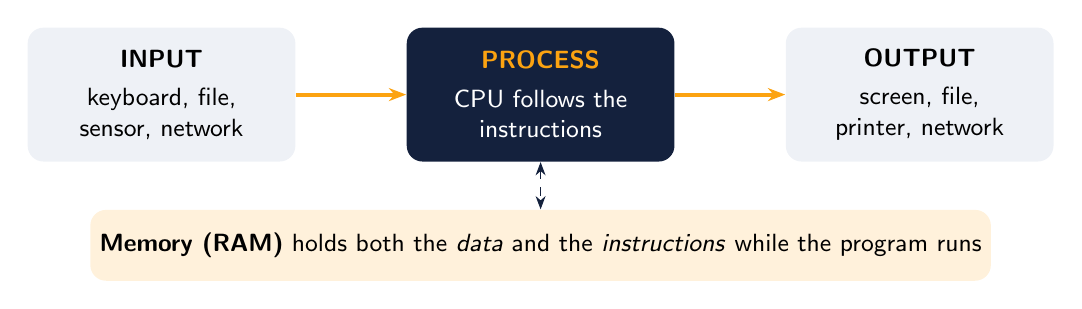
\begin{tikzpicture}[node distance=14mm,
  blk/.style={draw=none,rounded corners=2mm,minimum width=34mm,minimum height=17mm,align=center,font=\sffamily\small}]
\node[blk,fill=mist] (i) {\textbf{INPUT}\\[1mm] keyboard, file,\\ sensor, network};
\node[blk,fill=ink,text=white,right=of i] (p) {\textbf{\color{amber}PROCESS}\\[1mm] CPU follows the\\ instructions};
\node[blk,fill=mist,right=of p] (o) {\textbf{OUTPUT}\\[1mm] screen, file,\\ printer, network};
\draw[arr,draw=amber,line width=1.4pt] (i)--(p); \draw[arr,draw=amber,line width=1.4pt] (p)--(o);
\node[blk,fill=amber!15,below=6mm of p,minimum width=112mm,minimum height=9mm] (m) {\textbf{Memory (RAM)} holds both the \emph{data} and the \emph{instructions} while the program runs};
\draw[<->,>=Stealth,draw=ink,dashed] (p)--(m);
\end{tikzpicture}
\caption{The input--process--output model and the stored-program (von Neumann) idea.}\label{fig:ipo}
\end{figure}

The idea that the program's instructions are stored in the same memory as its data is due to John von Neumann (1945) and is still the architecture of every laptop and phone. RAM is \emph{volatile}: when the power is off it is empty, whereas files on a disk or SSD remain.

\subsection{Fast, but completely literal}
A single modern processor core executes on the order of $10^{9}$ simple instructions per second. Yet every one of those instructions belongs to only four families:
\begin{enumerate}[leftmargin=*,itemsep=1pt]
  \item \textbf{arithmetic} (add, subtract, multiply, divide),
  \item \textbf{comparison and logic} (is $a<b$? AND, OR, NOT),
  \item \textbf{data movement} (copy a value from memory to a register and back),
  \item \textbf{jumps} (continue at another instruction, possibly only if a condition holds).
\end{enumerate}
The computer never guesses what you \emph{meant}. It does exactly what it is told, in exactly the order it is told. Consequently:

\begin{defbox}[Key insight]
The difficult part of programming is not typing code. It is deciding the exact, unambiguous sequence of steps that solves the problem, the \textbf{algorithm}. The programming language only writes those steps in a form the machine can execute.
\end{defbox}

\subsection{From an idea to a running program}
Figure~\ref{fig:pipeline} shows what happens to your work. You write the first two boxes; the tools do the rest when you type \texttt{dotnet run}.

\begin{figure}[h]\centering
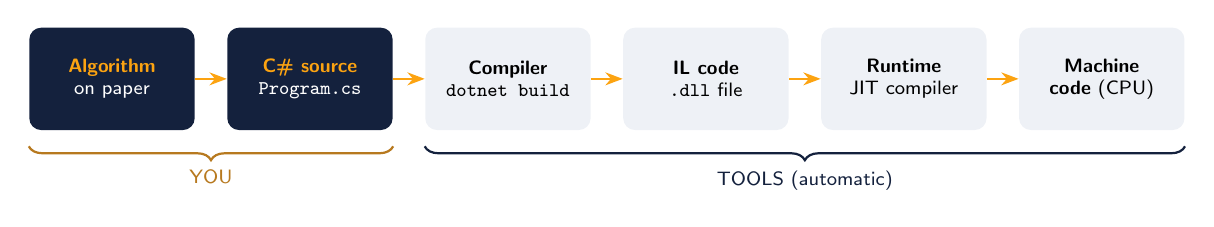
\begin{tikzpicture}[node distance=4mm,
  st/.style={rounded corners=1.5mm,minimum width=21mm,minimum height=13mm,align=center,font=\sffamily\scriptsize}]
\node[st,fill=ink,text=white] (a) {\textbf{\color{amber}Algorithm}\\ on paper};
\node[st,fill=ink,text=white,right=of a] (b) {\textbf{\color{amber}C\# source}\\ \texttt{Program.cs}};
\node[st,fill=mist,right=of b] (c) {\textbf{Compiler}\\ \texttt{dotnet build}};
\node[st,fill=mist,right=of c] (d) {\textbf{IL code}\\ \texttt{.dll} file};
\node[st,fill=mist,right=of d] (e) {\textbf{Runtime}\\ JIT compiler};
\node[st,fill=mist,right=of e] (f) {\textbf{Machine}\\ \textbf{code} (CPU)};
\foreach \x/\y in {a/b,b/c,c/d,d/e,e/f} \draw[arr,draw=amber] (\x)--(\y);
\draw[decorate,decoration={brace,mirror,amplitude=5pt},thick,amberdk] ([yshift=-2mm]a.south west)--([yshift=-2mm]b.south east) node[midway,below=5pt,font=\sffamily\scriptsize,amberdk]{YOU};
\draw[decorate,decoration={brace,mirror,amplitude=5pt},thick,ink] ([yshift=-2mm]c.south west)--([yshift=-2mm]f.south east) node[midway,below=5pt,font=\sffamily\scriptsize,ink]{TOOLS (automatic)};
\end{tikzpicture}
\caption{The C\# tool chain. IL = Intermediate Language; JIT = just-in-time compilation.}\label{fig:pipeline}
\end{figure}

The C\# compiler (called Roslyn) translates source code into \term{Intermediate Language} (IL), stored in a \texttt{.dll} file. When the program starts, the .NET runtime translates the IL into machine code for the actual processor (x64, ARM64, \dots). This is why the same compiled program runs on Windows, Linux and macOS.

\begin{table}[h]\centering\small
\begin{tabularx}{\linewidth}{lp{42mm}L}
\toprule
Level & Example: ``put 5 in a register, add 3'' & Characteristics\\ \midrule
Machine code (x86, hex) & \texttt{B8 05 00 00 00}\newline\texttt{83 C0 03} & The bytes the CPU actually reads. Practically unreadable for humans.\\
Assembly & \texttt{mov eax, 5}\newline\texttt{add eax, 3} & One mnemonic per machine instruction; tied to one processor family.\\
High-level (C\#) & \texttt{int sum = 5 + 3;} & Close to human thinking; portable across systems.\\ \bottomrule
\end{tabularx}
\caption{The same computation at three levels of abstraction.}
\end{table}

\begin{activity}[Think about it]
For each of the following, name the input, the process and the output: a pocket calculator; an ATM withdrawal; a navigation app computing a route; a thermostat.
\end{activity}

% =====================================================================
\section{What is an algorithm?}\label{sec:algorithm}

\subsection{The Exact Instructions Challenge}
In class we watch a short video in which children write instructions for making a sandwich, and their father follows them \emph{literally}: ``put the peanut butter on the bread'' results in the closed jar being placed on the loaf. While watching, note down (i)~which instruction was ambiguous, (ii)~which step was missing, (iii)~which step was in the wrong order, (iv)~whether the ``algorithm'' ever ended, and (v)~how the children fixed it. The father behaves exactly like a processor, and the children's cycle of \emph{write, test, fail, fix} is exactly how programs are developed.

\subsection{Definition}
\begin{defbox}[Definition -- Algorithm]
An \textbf{algorithm} is a \textcolor{amber}{\textbf{finite}} sequence of \textcolor{amber}{\textbf{well-defined}} steps that transforms a given \textcolor{amber}{\textbf{input}} into the desired \textcolor{amber}{\textbf{output}}, and then stops.
\end{defbox}

\paragraph{Where the word comes from.} Muhammad ibn Mūsā al-Khwārizmī (c.\,780--850) worked at the House of Wisdom in Baghdad. His book on calculating with Hindu--Arabic numerals introduced the decimal system to Europe, where his name was Latinised as \emph{Algoritmi}; hence \emph{algorithm}. The title of his other book, \emph{al-Jabr}, gave us the word \emph{algebra}.

\paragraph{Algorithm versus program.} An algorithm is an \emph{idea}, independent of any language; it can be written in words, in pseudocode or as a flowchart. A \term{program} is one \emph{implementation} of that idea in a particular programming language. One algorithm can be implemented in C\#, Python, Java or any other language: the relation is one-to-many. A recipe is an algorithm; the dish cooked in a particular kitchen is a program run.

\subsection{The five properties of an algorithm}
Following D.\,E.~Knuth, a procedure qualifies as an algorithm only if it has all five properties below.

\begin{center}\small
\begin{tabularx}{\linewidth}{>{\bfseries}p{27mm}L>{\leavevmode\itshape\color{errc}}p{47mm}}
\hrow \hdr{Property} & \hdr{Meaning} & \hdr{Violated by \dots}\\
Finiteness & It stops after a finite number of steps. & ``Keep stirring.'' (until when?)\\
\rowcolor{mist} Definiteness & Every step is precise and unambiguous. & ``Add some sugar.'' (how much?)\\
Input & It has zero or more clearly specified inputs. & ``Take the bread.'' (which bread?)\\
\rowcolor{mist} Output & It produces at least one result related to the input. & An empty plate.\\
Effectiveness & Every step is basic enough to be carried out exactly. & ``Make it tasty.''\\
\end{tabularx}
\end{center}

For practical programming we add a sixth requirement: \term{correctness}. The algorithm must produce the right output for \emph{every} valid input, including unusual ones (the \emph{edge cases}).

\subsection{Quiz: algorithm or not?}
Decide for each item whether it is an algorithm. If not, name the property that fails.
\begin{enumerate}[leftmargin=*,itemsep=1pt]
  \item The instructions on a shampoo bottle: ``Lather. Rinse. Repeat.''
  \item The long-division method you learned in primary school.
  \item ``Print the largest prime number.''
  \item A recipe step: ``Add salt to taste.''
  \item Finding a word in a paper dictionary by opening it near the word's first letter and moving forwards or backwards.
  \item ``Choose the best football team in the world.''
\end{enumerate}
\begin{notebox}[Answers]
(1)~No: it never stops (finiteness). (2)~Yes. (3)~No: Euclid proved that there are infinitely many primes, so no largest one exists; the procedure never finishes and produces no output. (4)~No: ``to taste'' is not precise (definiteness). (5)~Yes: the dictionary is finite and alphabetically ordered, so the search always ends. This is the idea behind \emph{binary search} (Week~10). (6)~No: there is no agreed criterion (definiteness, effectiveness).
\end{notebox}

\subsection{An everyday algorithm: brewing Turkish tea}
Compare the vague version ``boil water, add tea, serve'' with the precise version below. The colours mark the three kinds of structure discussed in the next subsection.

\begin{pseudobox}[Algorithm 1 -- Brewing Turkish tea]
\begin{enumerate}[leftmargin=*,itemsep=0pt]
  \item Fill the kettle (bottom pot) with 1\,L of water.
  \item Put 4 teaspoons of black tea into the teapot (top pot).
  \item Place the teapot on the kettle and turn the stove on.
  \item \textcolor{repc}{\textbf{WHILE} the water is not boiling: wait 1 minute.}
  \item Pour boiling water into the teapot until it is $\tfrac34$ full.
  \item Lower the heat and wait 15 minutes.
  \item \textcolor{selc}{\textbf{IF} the guest wants strong tea \textbf{THEN} fill the glass $\tfrac23$ with tea, \textbf{ELSE} fill it $\tfrac13$ with tea.}
  \item Top up the glass with hot water. \textbf{STOP}.
\end{enumerate}
\end{pseudobox}

\subsection{Three structures are enough}
Every algorithm can be built from only three control structures. This is the \term{structured program theorem} of B\"ohm and Jacopini (1966).

\begin{center}\small
\begin{tabularx}{\linewidth}{>{\bfseries}p{24mm}L>{\raggedright\arraybackslash}p{44mm}c}
\hrow \hdr{Structure} & \hdr{Meaning} & \hdr{Pseudocode example} & \hdr{C\# in}\\
\textcolor{seqc}{Sequence} & Steps executed one after another, top to bottom. & \READ $a$, $b$\newline $s\gets a+b$\newline \PRINT $s$ & Weeks 3--4\\
\rowcolor{mist}\textcolor{selc}{Selection} & Choose between paths according to a condition. & \textbf{IF} $age\ge 18$ \textbf{THEN}\newline\hspace*{3mm}\PRINT\str{adult}\newline\textbf{ELSE} \PRINT\str{minor} & Week 5\\
\textcolor{repc}{Repetition} & Repeat a block while a condition holds. & \textbf{WHILE} $i\le 10$\newline\hspace*{3mm}\PRINT $i$;\ $i\gets i+1$ & Weeks 6--7\\
\end{tabularx}
\end{center}
This theorem is why the course is ordered the way it is: after sequence, selection and repetition you have, in principle, everything needed to express any computation.

\subsection{Four ways to write an algorithm}
The same algorithm, ``read a number and print its absolute value'', can be written in four ways:

\begin{center}
\begin{minipage}[t]{0.47\linewidth}
\textbf{(a) Natural language.} \emph{Read the number. If it is negative, remove its minus sign. Show the number.}\\[1mm]
{\small Easy for anyone to read, but often ambiguous.}

\medskip
\textbf{(b) Pseudocode.}\vspace{-2mm}
\begin{pseudobox}
\begin{algorithmic}[1]
\START
\State \READ $x$
\IfX{$x<0$}
  \State $x \gets -x$
\EndIfX
\State \PRINT $x$
\STOP
\end{algorithmic}
\end{pseudobox}
{\small Precise and needs no tools; our main notation on paper.}
\end{minipage}\hfill
\begin{minipage}[t]{0.47\linewidth}
\textbf{(c) Flowchart} (Week~2).\\[1mm]
\centering
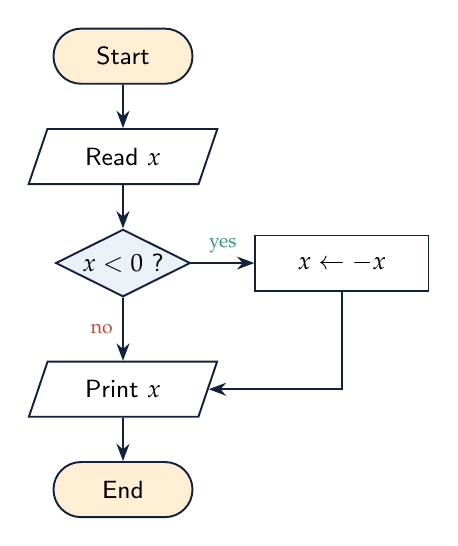
\begin{tikzpicture}[node distance=5.5mm]
\node[term] (s) {Start};
\node[io,below=of s] (r) {Read $x$};
\node[dec,below=of r] (d) {$x<0$ ?};
\node[proc,right=8mm of d] (n) {$x \gets -x$};
\node[io,below=8mm of d] (p) {Print $x$};
\node[term,below=of p] (e) {End};
\draw[arr] (s)--(r); \draw[arr] (r)--(d);
\draw[arr] (d)--node[above,font=\scriptsize,repc]{yes}(n);
\draw[arr] (d)--node[left,font=\scriptsize,errc]{no}(p);
\draw[arr] (n)|-(p);
\draw[arr] (p)--(e);
\end{tikzpicture}
\end{minipage}
\end{center}

\needspace{8\baselineskip}
\textbf{(d) C\# code} (Week~3 onwards). Executable, but with strict syntax:
\begin{lstlisting}
int x = int.Parse(Console.ReadLine());
if (x < 0)
    x = -x;
Console.WriteLine(x);
\end{lstlisting}

\subsection{Pseudocode conventions for MCMP113}\label{sec:conventions}
There is no single standard pseudocode. In this course, in all slides, homework and exams, we use the following conventions.

\begin{center}\small
\begin{tabularx}{\linewidth}{>{\ttfamily\bfseries}p{47mm}Lp{44mm}}
\hrow \hdr{Keyword} & \hdr{Meaning} & \hdr{Example}\\
START \dots\ END & beginning and end of the algorithm & \\
\rowcolor{mist} READ x & input: get a value from the user & \READ $age$\\
PRINT \dots & output: show a value or a message & \PRINT \str{Total:}, $sum$\\
\rowcolor{mist} x $\gets$ expression & assignment: evaluate the right-hand side, store it in $x$ & $total \gets total + price$\\
IF c THEN \dots\ ELSE \dots\ END IF & selection & \textbf{IF} $age\ge 18$ \textbf{THEN} \dots\\
\rowcolor{mist} WHILE c \dots\ END WHILE & repeat while condition $c$ is true & \textbf{WHILE} $i \le N$\\
FOR i $\gets$ a TO b \dots\ END FOR & repeat for $i=a,a+1,\dots,b$ & \textbf{FOR} $i\gets 1$ \textbf{TO} $10$\\
\rowcolor{mist} + \ $-$ \ $\times$ \ / \ mod & arithmetic; \texttt{mod} is the remainder & $17 \MOD 5 = 2$\\
= \ $\neq$ \ < \ $\le$ \ > \ $\ge$ & comparison (result: true or false) & \textbf{IF} $x\ne 0$ \textbf{THEN} \dots\\
\rowcolor{mist} AND \ OR \ NOT & combine conditions & \textbf{IF} $a>0$ \AND $b>0$\\
\end{tabularx}
\end{center}

\begin{warnbox}[The number-one beginner trap: assignment is not equality]
In pseudocode, $\gets$ \emph{assigns} and $=$ \emph{compares}. In C\#, \texttt{=} assigns and \texttt{==} compares. The statement $x \gets x+1$ is not an equation (as an equation, $x=x+1$ has no solution). It means ``the new value of $x$ is the old value of $x$ plus one''.
\end{warnbox}

% =====================================================================
\section{Problem-solving steps}\label{sec:problem}

\subsection{The five-step method}
Inspired by G.~P\'olya's \emph{How to Solve It} (1945), we solve every programming problem in five steps:
\begin{enumerate}[leftmargin=*,itemsep=2pt]
  \item \term{Understand (analyse).} What is given (input)? What is asked (output)? What are the constraints? Which unusual inputs can occur?
  \item \term{Design.} Write the algorithm: numbered steps, then pseudocode and/or a flowchart.
  \item \term{Implement.} Translate the algorithm into C\#.
  \item \term{Test and debug.} Run the program (or trace the algorithm by hand) with normal, boundary and invalid inputs.
  \item \term{Document.} Comments, meaningful names, notes for other people and for your future self.
\end{enumerate}
The method is a \emph{cycle}, not a straight line: a failed test sends you back to Design, or even to Understand. Beginners tend to spend most of their time in step~3; experienced programmers spend most of it in steps~1--2, which is why their step~4 is short.

\begin{notebox}[Rule of thumb]
Do not start coding until you can explain your algorithm in your own words to a classmate.
\end{notebox}

\subsection{Worked example 1: average of three exam grades}
\textbf{Problem.} A student enters three exam grades (0--100). Show the average and whether the student passed (average at least 50).

\subsubsection{Step 1 -- Understand: the IPO table}
\begin{center}\small
\begin{tabularx}{\linewidth}{LLL}
\hrow \hdr{Input} & \hdr{Process} & \hdr{Output}\\
$g_1, g_2, g_3$ (numbers, $0$--$100$) & $avg \gets (g_1+g_2+g_3)/3$; compare $avg$ with $50$ & $avg$; \str{PASSED} or \str{FAILED}\\ \bottomrule
\end{tabularx}
\end{center}
Questions to ask \emph{before} designing:
\begin{itemize}[leftmargin=*,itemsep=0pt]
  \item Can a grade be $72.5$, or only whole numbers? (This decides the data type in Week~3.)
  \item What if the user types $120$ or $-5$? (Needs a range check, i.e.\ selection, Week~5.)
  \item Is exactly $50$ a pass? (Decides between $\ge$ and $>$.)
  \item Do all exams have equal weight? (If not, a weighted average is needed.)
\end{itemize}

\subsubsection{Step 2 -- Design}
In plain language: (1) start; (2) read the three grades; (3) add them and divide by 3; (4) show the average; (5) if the average is at least 50 show ``PASSED'', otherwise ``FAILED''; (6) stop. In pseudocode:

\begin{pseudobox}[Algorithm 2 -- Average of three grades]
\begin{algorithmic}[1]
\START
\State \READ $g_1, g_2, g_3$
\State $avg \gets (g_1 + g_2 + g_3)/3$
\State \PRINT $avg$
\IfX{$avg \ge 50$}
  \State \PRINT \str{PASSED}
\ElseX
  \State \PRINT \str{FAILED}
\EndIfX
\STOP
\end{algorithmic}
\end{pseudobox}

\begin{warnbox}[Parentheses matter]
Writing $g_1 + g_2 + g_3/3$ is a different algorithm: division is performed before addition, so it computes $g_1+g_2+\frac{g_3}{3}$. For $60, 70, 80$ the correct average is $70$, whereas the wrong formula gives $156.67$. Operator precedence is studied in Week~4.
\end{warnbox}

\subsubsection{Step 4 -- Test: choosing good test cases}
Testing with a single ``nice'' input proves very little. Choose tests that are most likely to break the algorithm:
\begin{center}\small
\begin{tabularx}{\linewidth}{>{\bfseries}p{27mm}p{28mm}L}
\hrow \hdr{Kind of test} & \hdr{$g_1,g_2,g_3$} & \hdr{Expected result}\\
Normal & $60, 70, 80$ & $70.00$ -- PASSED\\
\rowcolor{mist} Boundary & $50, 50, 50$ & $50.00$ -- PASSED\\
Just below & $49, 50, 50$ & $49.67$ -- FAILED \quad ($149/3 = 49.\overline{6}$)\\
\rowcolor{mist} Maximum & $100, 100, 100$ & $100.00$ -- PASSED\\
Minimum & $0, 0, 0$ & $0.00$ -- FAILED\\
\rowcolor{mist} Out of range & $120, 70, 80$ & \textcolor{errc}{should be rejected, but Algorithm~2 prints $90.00$}\\
Wrong type & \texttt{abc}, $70$, $80$ & \textcolor{errc}{a C\# program would crash (\texttt{FormatException})}\\
\end{tabularx}
\end{center}
Boundary tests catch the most errors (for example, writing $avg>50$ instead of $avg\ge50$). The last two rows reveal \emph{missing requirements}: Algorithm~2 does not validate its input. As Dijkstra put it: \emph{``Program testing can be used to show the presence of bugs, but never to show their absence.''}

\subsection{Worked example 2: the sum $1+2+\dots+N$ and trace tables}
\begin{pseudobox}[Algorithm 3 -- Sum of the first $N$ positive integers]
\begin{algorithmic}[1]
\START
\State \READ $N$
\State $sum \gets 0$
\State $i \gets 1$
\WhileX{$i \le N$}
  \State $sum \gets sum + i$
  \State $i \gets i + 1$
\EndWhileX
\State \PRINT $sum$
\STOP
\end{algorithmic}
\end{pseudobox}

A \term{trace table} (also called a \emph{desk check}) executes the algorithm by hand: one column per variable, one row per pass through the loop. For $N=5$:
\begin{center}\small
\begin{tabular}{cccc}
\toprule
pass & $i$ (before test) & $i\le N$? & $sum$ (after pass)\\ \midrule
start & 1 & -- & 0\\
1 & 1 & yes & 1\\
2 & 2 & yes & 3\\
3 & 3 & yes & 6\\
4 & 4 & yes & 10\\
5 & 5 & yes & 15\\
exit & 6 & \textcolor{errc}{no} & \textbf{15}\\ \bottomrule
\end{tabular}
\end{center}
\textbf{Checks.} \emph{Termination:} $i$ increases by one in every pass, so it eventually exceeds $N$. \emph{Edge cases:} for $N=0$ the loop body never runs and the output is $0$, which is correct; for negative $N$ the output is also $0$ -- is that what the user expects?

\paragraph{A different algorithm for the same problem.} The young Gauss is said to have noticed that pairing the first and last terms gives $N+1$ each time:
\begin{equation}
S = \sum_{i=1}^{N} i, \qquad 2S = \underbrace{(1+N) + (2+(N-1)) + \dots + (N+1)}_{N \text{ pairs, each equal to } N+1} = N(N+1)
\quad\Longrightarrow\quad S = \frac{N(N+1)}{2}.
\end{equation}
For $N=5$: $S = 5\cdot 6/2 = 15$. Algorithm~3 needs $N$ loop passes, the formula needs one multiplication and one division, whatever $N$ is. For $N=10^{9}$ the difference is dramatic. \emph{Choosing the better algorithm is a design decision, not a coding one.}

\subsection{Worked example 3: guess my number -- efficiency}
I think of an integer between $1$ and $1000$; you guess, and I answer ``higher'', ``lower'' or ``correct''.
\begin{itemize}[leftmargin=*,itemsep=0pt]
  \item \textbf{Strategy A (linear):} guess $1, 2, 3, \dots$. Worst case: $1000$ guesses.
  \item \textbf{Strategy B (halving):} always guess the middle of the remaining range. Every answer halves the range, so after $k$ guesses at most $\lfloor 1000/2^{k}\rfloor$ candidates remain. The worst case is
  \begin{equation}
  k_{\max} = \lceil \log_2 (N+1) \rceil, \qquad N = 1000 \;\Rightarrow\; k_{\max} = 10, \quad\text{since } 2^{10}=1024 \ge 1001 .
  \end{equation}
\end{itemize}

\begin{pseudobox}[Algorithm 4 -- Guessing by halving]
\begin{algorithmic}[1]
\START
\State $low \gets 1$;\ \ $high \gets 1000$;\ \ $found \gets$ false
\WhileX{\NOT $found$}
  \State $guess \gets \lfloor (low + high)/2 \rfloor$
  \State \PRINT $guess$;\ \ \READ $answer$
  \IfX{$answer = \str{correct}$}
    \State $found \gets$ true
  \ElseX
    \IfX{$answer = \str{higher}$}
      \State $low \gets guess + 1$
    \ElseX
      \State $high \gets guess - 1$
    \EndIfX
  \EndIfX
\EndWhileX
\STOP
\end{algorithmic}
\end{pseudobox}

Trace for the secret number $737$ (10 guesses):
\begin{center}\small
\begin{tabular}{c*{10}{c}}
\toprule
guess no. & 1 & 2 & 3 & 4 & 5 & 6 & 7 & 8 & 9 & 10\\ \midrule
guess & 500 & 750 & 625 & 687 & 718 & 734 & 742 & 738 & 736 & \textbf{737}\\
answer & $\uparrow$ & $\downarrow$ & $\uparrow$ & $\uparrow$ & $\uparrow$ & $\uparrow$ & $\downarrow$ & $\downarrow$ & $\uparrow$ & \textcolor{repc}{\checkmark}\\ \bottomrule
\end{tabular}
\end{center}

\begin{center}\small
\begin{tabular}{lrrrr}
\toprule
Range size $N$ & $100$ & $1\,000$ & $10^{6}$ & $10^{9}$\\ \midrule
Strategy A, worst case & $100$ & $1\,000$ & $1\,000\,000$ & $1\,000\,000\,000$\\
Strategy B, worst case & $7$ & $10$ & $20$ & $30$\\ \bottomrule
\end{tabular}
\end{center}
Strategy A takes time proportional to $N$ (we write $O(N)$); strategy B takes time proportional to $\log_2 N$ ($O(\log N)$). Strategy B is \term{binary search}, which we implement on arrays in Week~10.

\subsection{Worked example 4: Euclid's greatest common divisor}
Written down around 300\,BC in Euclid's \emph{Elements}, this is one of the oldest non-trivial algorithms still in use; it is part of the arithmetic behind public-key cryptography (RSA) used in secure HTTPS connections.

\begin{pseudobox}[Algorithm 5 -- Euclid's GCD]
\begin{algorithmic}[1]
\START
\State \READ $a, b$ \Comment{positive integers}
\WhileX{$b \ne 0$}
  \State $r \gets a \MOD b$
  \State $a \gets b$
  \State $b \gets r$
\EndWhileX
\State \PRINT $a$
\STOP
\end{algorithmic}
\end{pseudobox}

\begin{center}\small
\begin{tabular}{ccc}
\toprule
$a$ & $b$ & $r = a \MOD b$\\ \midrule
48 & 18 & 12\\
18 & 12 & 6\\
12 & 6 & 0\\
\textcolor{repc}{\textbf{6}} & \textcolor{repc}{0} & stop: $\gcd(48,18)=6$\\ \bottomrule
\end{tabular}
\end{center}
\textbf{Why it is correct.} Any common divisor of $a$ and $b$ also divides $r=a-qb$, and any common divisor of $b$ and $r$ also divides $a=qb+r$; hence $\gcd(a,b)=\gcd(b,\,a \MOD b)$. \textbf{Why it terminates.} Since $0 \le r < b$, the value of $b$ strictly decreases in every pass and, being a non-negative integer, must reach $0$. If the input has $a<b$, the first pass simply swaps them: for $(18,48)$ we get $r=18$, $a=48$, $b=18$.

\subsection{Worked example 5: an algorithm in your wallet -- T.C. Kimlik No}
The 11-digit Turkish identity number $d_1d_2\dots d_{11}$ contains two \emph{check digits}. The rules are:
\begin{align}
& d_1 \neq 0, \\
& d_{10} = \Big( 7\,(d_1+d_3+d_5+d_7+d_9) - (d_2+d_4+d_6+d_8) \Big) \MOD 10, \\
& d_{11} = \Big( d_1 + d_2 + \dots + d_{10} \Big) \MOD 10 .
\end{align}
\textbf{Worked example} with the \emph{made-up} first nine digits $1\,2\,3\,4\,5\,6\,7\,8\,9$: the odd-position sum is $25$, the even-position sum is $20$, so $d_{10} = (175-20) \MOD 10 = 155 \MOD 10 = 5$, and $d_{11}=(45+5)\MOD 10 = 0$. The full number is $12345678950$. It passes the check but belongs to nobody.

\textbf{Why it is useful.} If exactly one of $d_1,\dots,d_{10}$ is mistyped, the sum $d_1+\dots+d_{10}$ changes by a non-zero amount between $-9$ and $+9$, so its remainder modulo~10 no longer equals $d_{11}$. The error is detected instantly, without contacting any database. The same idea protects IBANs (mod~97), EAN-13 product barcodes and credit-card numbers (the Luhn algorithm).

\begin{notebox}[Looking ahead to Week 4]
The expression $7\cdot(\text{odd sum}) - (\text{even sum})$ can be negative (e.g.\ $7\cdot 1 - 36 = -29$). Mathematically $-29 \MOD 10 = 1$, but the C\# operator \texttt{\%} gives $-29 \,\%\, 10 = -9$. A correct C\# version must use \texttt{((x \% 10) + 10) \% 10}.
\end{notebox}

\subsection{Common mistakes: bad algorithm, good algorithm}
\begin{center}\small
\begin{tabularx}{\linewidth}{>{\bfseries\raggedright\arraybackslash}p{30mm}>{\raggedright\arraybackslash\leavevmode\color{errc}}p{46mm}>{\raggedright\arraybackslash\leavevmode\color{repc!80!black}}L}
\hrow \hdr{Problem} & \hdr{Bad} & \hdr{Good}\\
Ambiguous step & ``Divide the numbers.'' & $avg \gets (g_1+g_2+g_3)/3$\\
\rowcolor{mist} No termination & ``Keep asking for a password.'' & Ask at most 3 times, then lock the account.\\
Missing edge case & $result \gets a/b$ & \textbf{IF} $b=0$ \textbf{THEN} \PRINT\str{error} \textbf{ELSE} $result\gets a/b$\\
\rowcolor{mist} Wrong order & \PRINT $sum$, then $sum \gets a+b$ & $sum \gets a+b$, then \PRINT $sum$\\
Undefined input & ``Read the grade.'' & Read a grade in $[0,100]$; reject other values.\\
\end{tabularx}
\end{center}
Each row violates one property: definiteness, finiteness, correctness, sequence and input specification, respectively.

\subsection{Sneak peek: the same algorithm in C\#}
In Week~3 you will write Algorithm~2 as follows. You do not need to understand the syntax yet; notice only that every pseudocode line maps to one or two lines of code.
\begin{lstlisting}
Console.Write("Grade 1: ");
double g1 = double.Parse(Console.ReadLine());
Console.Write("Grade 2: ");
double g2 = double.Parse(Console.ReadLine());
Console.Write("Grade 3: ");
double g3 = double.Parse(Console.ReadLine());

double avg = (g1 + g2 + g3) / 3;          // parentheses!
Console.WriteLine($"Average: {avg:F2}");

if (avg >= 50)
    Console.WriteLine("PASSED");
else
    Console.WriteLine("FAILED");
\end{lstlisting}
\begin{center}\small
\begin{tabular}{ll}
\toprule
Pseudocode & C\#\\ \midrule
\READ $x$ & \texttt{Console.ReadLine()} (plus a conversion such as \texttt{double.Parse})\\
\PRINT $x$ & \texttt{Console.WriteLine(x)}\\
$x \gets e$ & \texttt{x = e;}\\
\textbf{IF} $c$ \textbf{THEN} \dots\ \textbf{ELSE} \dots & \texttt{if (c) \{ \dots \} else \{ \dots \}}\\ \bottomrule
\end{tabular}
\end{center}
\begin{notebox}[Turkish-locale computers]
On a computer set to Turkish regional settings, \texttt{double.Parse} expects a decimal \emph{comma} ($72{,}5$), not a point. We will handle this properly in Week~3.
\end{notebox}

% =====================================================================
\needspace{12\baselineskip}
\section{Summary}\label{sec:summary}
\begin{enumerate}[leftmargin=*,itemsep=1pt]
  \item An \term{algorithm} is a finite, precise recipe that turns input into output and stops.
  \item Its five properties are finiteness, definiteness, input, output and effectiveness; in practice we also require correctness.
  \item Every algorithm is built from \textcolor{seqc}{\textbf{sequence}}, \textcolor{selc}{\textbf{selection}} and \textcolor{repc}{\textbf{repetition}}.
  \item Algorithms can be written in natural language, pseudocode, flowcharts or code.
  \item Solve problems in five steps: understand, design, implement, test, document, and loop back when a test fails.
  \item Trace tables and well-chosen test cases (normal, boundary, invalid) find errors before the computer does.
  \item Different algorithms for the same problem can differ enormously in efficiency (sum formula; binary search).
\end{enumerate}

\subsection*{Glossary (English -- Turkish)}
\begin{center}\small
\begin{tabular}{ll@{\hspace{10mm}}ll}
\toprule
algorithm & algoritma & input / output & girdi / çıktı\\
step & adım & assignment & atama\\
pseudocode & sözde kod & condition & koşul\\
flowchart & akış şeması & selection (decision) & seçim (karar)\\
sequence & sıralı yapı & repetition (loop) & tekrar (döngü)\\
variable & değişken & trace table & izleme tablosu\\
finiteness & sonluluk & edge / boundary case & sınır durumu\\
definiteness & belirlilik / kesinlik & remainder (mod) & kalan (mod)\\
effectiveness & etkinlik / yapılabilirlik & greatest common divisor & en büyük ortak bölen (EBOB)\\
compiler & derleyici & check digit & kontrol basamağı\\
source code & kaynak kod & efficiency & verimlilik\\
bug / debugging & hata / hata ayıklama & binary search & ikili arama\\ \bottomrule
\end{tabular}
\end{center}

% =====================================================================
\section{Exercises}\label{sec:exercises}
For every exercise: write the IPO table, the numbered steps and the pseudocode (using the conventions of Section~\ref{sec:conventions}), then trace your algorithm with at least one normal and one edge-case input. Difficulty: \stars{1} basic, \stars{2} intermediate, \stars{3} challenging.

\subsection{In-class exercises (groups of 2--3)}
\begin{enumerate}[label=\textbf{\Alph*.},leftmargin=*,itemsep=3pt]
  \item \stars{1} \textbf{Even or odd.} Read an integer; print whether it is even or odd.
  \solution{$n$ is even exactly when $n \MOD 2 = 0$.
  \begin{algorithmic}[1]
  \START \State \READ $n$
  \IfX{$n \MOD 2 = 0$} \State \PRINT \str{even} \ElseX \State \PRINT \str{odd} \EndIfX \STOP
  \end{algorithmic}
  Tests: $7\to$ odd, $10\to$ even, $0\to$ even. (For negative $n$ the C\# \texttt{\%} gives $-1$ for odd numbers, so test ``$\ne 0$'' rather than ``$=1$''.)}

  \item \stars{2} \textbf{Leap year.} Read a year; it is a leap year if it is divisible by 4 and not by 100, or if it is divisible by 400.
  \solution{
  \begin{algorithmic}[1]
  \START \State \READ $y$
  \IfX{($y \MOD 4 = 0$ \AND $y \MOD 100 \ne 0$) \OR $y \MOD 400 = 0$}
    \State \PRINT \str{leap year}
  \ElseX \State \PRINT \str{not a leap year} \EndIfX \STOP
  \end{algorithmic}
  Tests: $2024$ leap; $2023$ not; $1900$ not (divisible by 100 but not 400); $2000$ leap (divisible by 400).}

  \item \stars{2} \textbf{ATM withdrawal.} Given the account balance and a requested amount, allow the withdrawal only if the balance is sufficient and the amount is a positive multiple of 10; print the new balance or a reason for refusal.
  \solution{
  \begin{algorithmic}[1]
  \START \State \READ $balance$, $amount$
  \IfX{$amount \le 0$ \OR $amount \MOD 10 \ne 0$}
    \State \PRINT \str{invalid amount}
  \ElseX
    \IfX{$amount > balance$} \State \PRINT \str{insufficient funds}
    \ElseX \State $balance \gets balance - amount$ \State \PRINT \str{new balance:}, $balance$ \EndIfX
  \EndIfX \STOP
  \end{algorithmic}
  Tests: $(500,200)\to 300$; $(500,500)\to 0$ (boundary); $(500,510)\to$ insufficient; $(500,25)\to$ invalid; $(500,-10)\to$ invalid.}

  \item \stars{1} \textbf{Countdown.} Read $N$; print $N, N-1, \dots, 1$ and then ``Go!''.
  \solution{
  \begin{algorithmic}[1]
  \START \State \READ $N$
  \WhileX{$N \ge 1$} \State \PRINT $N$ \State $N \gets N - 1$ \EndWhileX
  \State \PRINT \str{Go!} \STOP
  \end{algorithmic}
  Trace $N=3$: prints $3,2,1$, Go!. Edge case $N=0$: prints only ``Go!''.}

  \item \stars{2} \textbf{Guess the number.} The computer holds a secret number; the user guesses repeatedly and receives ``higher'' or ``lower'' until correct. Also count the guesses.
  \solution{
  \begin{algorithmic}[1]
  \START \State $secret \gets$ a number between 1 and 100 \State $count \gets 0$ \State $guess \gets 0$
  \WhileX{$guess \ne secret$}
    \State \READ $guess$ \State $count \gets count + 1$
    \IfX{$guess < secret$} \State \PRINT \str{higher}
    \ElseX \IfX{$guess > secret$} \State \PRINT \str{lower} \EndIfX \EndIfX
  \EndWhileX
  \State \PRINT \str{correct after}, $count$, \str{guesses} \STOP
  \end{algorithmic}
  $guess$ is initialised to $0$ (outside the range) so that the loop runs at least once. In C\# this is a natural \texttt{do-while} (Week~7).}

  \item \stars{1} \textbf{Temperature conversion.} Read a temperature $C$ in degrees Celsius and print it in Fahrenheit, $F = \frac{9}{5}C + 32$.
  \solution{Sequence only: \READ $C$;\ $F \gets C \times 9/5 + 32$;\ \PRINT $F$. Tests: $0\to 32$, $100\to 212$, $-40\to -40$ (the two scales meet at $-40$).}
\end{enumerate}

\subsection{Homework (due before Week 2)}
\begin{enumerate}[label=\textbf{H\arabic*.},leftmargin=*,itemsep=3pt]
  \item Complete the two in-class exercises that your group did not do in class.
  \item \stars{1} Write an algorithm for a daily task of your choice that contains at least one \textbf{IF} and one \textbf{WHILE}.
  \item \stars{1} Trace Euclid's algorithm (Algorithm~5) for $(84, 36)$ in a table.
  \solution{$84 \MOD 36 = 12$; $36 \MOD 12 = 0$; so $\gcd(84,36)=12$ after two passes.}
  \item Install the .NET 10 SDK, VS Code and the C\# Dev Kit; run the four commands of Section~1.4 and post a screenshot of the output to the Telegram group.
\end{enumerate}

\subsection{Extra practice}
\begin{enumerate}[label=\textbf{P\arabic*.},leftmargin=*,itemsep=3pt]
  \item \stars{1} Trace Algorithm~3 for $N=3$ and for $N=0$. How many times is the loop condition tested in each case?
  \solution{$N=3$: output $6$; the condition is tested $4$ times ($i=1,2,3$ true; $i=4$ false). $N=0$: output $0$; tested once. In general the condition is tested $N+1$ times for $N\ge0$.}
  \item \stars{1} Use Gauss's formula to compute $1+2+\dots+100$ and $1+2+\dots+1000$.
  \solution{$100\cdot101/2 = 5050$; $1000\cdot1001/2 = 500\,500$.}
  \item \stars{2} What is the worst-case number of guesses with the halving strategy for a secret number between 1 and 500? Between 1 and 1\,000\,000?
  \solution{$\lceil\log_2 501\rceil = 9$ (since $2^9=512\ge501$); $\lceil\log_2 1\,000\,001\rceil = 20$ (since $2^{20}=1\,048\,576$).}
  \item \stars{2} Trace Euclid's algorithm for $(18,48)$ and for $(1071,462)$.
  \solution{$(18,48)$: rows $(18,48,18)$, $(48,18,12)$, $(18,12,6)$, $(12,6,0)$; result $6$. $(1071,462)$: rows $(1071,462,147)$, $(462,147,21)$, $(147,21,0)$; result $21$.}
  \item \stars{2} Compute the two check digits for the made-up first nine digits $2\,0\,2\,6\,1\,0\,0\,1\,5$.
  \solution{Odd positions: $2+2+1+0+5=10$; even positions: $0+6+0+1=7$. $d_{10} = (70-7)\MOD 10 = 63 \MOD 10 = 3$. $d_{11} = (17+3)\MOD 10 = 0$. Full number: $20261001530$.}
  \item \stars{2} \textbf{Find the bug.} A student wrote \quad $avg \gets g_1 + g_2 + g_3 / 3$ \quad and tested it only with $0,0,0$. Explain why the test passed and give a test that exposes the bug.
  \solution{For $0,0,0$ both formulas give $0$, so this test cannot tell them apart. Any non-zero input exposes it, e.g.\ $60,70,80$: correct $70$, buggy $156.67$. Lesson: a single ``trivial'' test is not enough.}
  \item \stars{2} \textbf{Maximum of $N$ numbers.} Read $N$ and then $N$ numbers one by one; print the largest. (Hint: keep a ``largest so far''.)
  \solution{
  \begin{algorithmic}[1]
  \START \State \READ $N$ \State \READ $x$ \State $max \gets x$ \State $i \gets 2$
  \WhileX{$i \le N$} \State \READ $x$ \IfX{$x > max$} \State $max \gets x$ \EndIfX \State $i \gets i+1$ \EndWhileX
  \State \PRINT $max$ \STOP
  \end{algorithmic}
  Initialising $max$ with the \emph{first} number (not with $0$) makes the algorithm correct also when all numbers are negative.}
  \item \stars{3} \textbf{Sum of digits.} Read a positive integer and print the sum of its digits (e.g.\ $4071 \to 12$). Use only $\MOD$, integer division and a loop.
  \solution{
  \begin{algorithmic}[1]
  \START \State \READ $n$ \State $s \gets 0$
  \WhileX{$n > 0$} \State $s \gets s + (n \MOD 10)$ \State $n \gets \lfloor n/10 \rfloor$ \EndWhileX
  \State \PRINT $s$ \STOP
  \end{algorithmic}
  Trace $4071$: $n=4071,\,s=1$; $n=407,\,s=8$; $n=40,\,s=8$; $n=4,\,s=12$; $n=0$ stop.}
  \item \stars{3} \textbf{Convert.} Rewrite the Turkish-tea algorithm (Algorithm~1) using the pseudocode conventions of Section~\ref{sec:conventions}, with variables for the water temperature and the guest's preference.
\end{enumerate}

% =====================================================================
\section*{References and further reading}
\addcontentsline{toc}{section}{References and further reading}
\begin{enumerate}[label={[\arabic*]},leftmargin=*,itemsep=1pt,font=\small]\small
  \item D.\,E. Knuth, \emph{The Art of Computer Programming, Vol.~1: Fundamental Algorithms}, 3rd ed., Addison-Wesley, 1997, Section~1.1.
  \item G. P\'olya, \emph{How to Solve It}, Princeton University Press, 1945.
  \item C. B\"ohm and G. Jacopini, ``Flow diagrams, Turing machines and languages with only two formation rules'', \emph{Communications of the ACM} 9(5), 366--371, 1966. \url{https://doi.org/10.1145/355592.365646}
  \item E.\,W. Dijkstra, ``Notes on Structured Programming'' (EWD249), 1970. \url{https://www.cs.utexas.edu/~EWD/ewd02xx/EWD249.PDF}
  \item T.\,H. Cormen, C.\,E. Leiserson, R.\,L. Rivest, C. Stein, \emph{Introduction to Algorithms}, 4th ed., MIT Press, 2022, Chapter~1.
  \item Microsoft, \emph{C\# documentation -- tutorials for beginners}. \url{https://learn.microsoft.com/en-us/dotnet/csharp/tour-of-csharp/tutorials/}
  \item Microsoft, \emph{.NET download (.NET 10)}. \url{https://dotnet.microsoft.com/en-us/download/dotnet/10.0}
\end{enumerate}

\end{document}
